\newpage
\documentclass[../SustainableHEP.tex]{subfiles}
\graphicspath{{\subfix{Sections/Figs/}}}
\begin{document}
\RaggedRight
\sloppy

%%%%%%%%%%%%%%%%%%%%%%%%%%%%%%%%%%%%%%%%%%%%%%%%%%

\section*{Outline}
\addcontentsline{toc}{section}{Outline}

The aims of this document are:
\begin{itemize}
    \item To improve awareness of the impact that high energy physics, cosmology and astroparticle physics, and hadron and nuclear physics (\acrshort{hecap}) has on the environment.
    \item To provide suggestions and encourage immediate action on ways that we, as a community, can play our part in limiting further degradation of the world's climate and ecosystems.
    \item To provide impetus for ongoing and collective discussions of how we can make positive changes to our community's work practices, in terms of environmental sustainability and for the issues of social justice from which climate change and environmental degradation cannot be disentangled.
\end{itemize}
The aims are not to stipulate the research that our communities should undertake, nor to debate its intrinsic value.

The discussions are divided into seven sections. Sections 2 through 7 cover the topics of Computing, Energy, Food, Mobility, Research Infrastructure and Technology, and Resources and Waste. Each of these sections contains a set of recommendations, for individuals, groups and institutions, and these are followed by longer discussions that include case studies and best practice examples, which can be read independently of the surrounding material. Collated lists of acronyms and abbreviations, best practices, case studies, and figures and tables are included at the end of this document.

\sref{sec:Introduction}, Preliminaries, begins by acknowledging the climate crisis and the environmental impacts of HECAP+ research. It provides a summary of the United Nations (UN) Sustainable Development Goals (\acrshort{sdg}s) and how these relate to \ACR\ research, and briefly reviews similar and complementary documents.

%%%%%%%%%%%%%%%%%%%%%%%%%%%%%%%%%%%%%%%%%%%%%%%%%%

\newpage

\section{Preliminaries}
\label{sec:Introduction}

\subsection{Introduction}

The 2021 report of the Intergovernmental Panel on Climate Change (\acrshort{ipcc})~\cite{IPCC2021report} is emphatic in its statements about the current status of the climate and the damaging impact that humanity continues to have upon it~\cite{IPCC2021reportSPM}:
\begin{quotation}
"It is unequivocal that human influence has warmed the atmosphere, ocean and land. Widespread and rapid changes in the atmosphere, ocean, cryosphere and biosphere have occurred.\ [\dots]\ Human-induced climate change is already affecting many weather and climate extremes in every region 
across the globe. Evidence of observed changes in extremes such as heatwaves, heavy precipitation, droughts, 
and tropical cyclones, and, in particular, their attribution to human influence, has strengthened since [the Fifth Assessment Report in 2014]."
\end{quotation}
It is also clear on the consequences of further inaction~\cite{IPCC2021reportSPM}:
\begin{quotation}
"Global surface temperature will continue to increase until at least mid-century under all emissions scenarios
considered. Global warming of 1.5\degree C and 2\degree C will be exceeded during the 21$^\text{st}$ century unless deep reductions 
in $\mathrm{CO_2}$ and other greenhouse gas emissions occur in the coming decades.\ [\dots]\ Many changes in the climate system become larger in direct relation to increasing global warming. They 
include increases in the frequency and intensity of hot extremes, marine heatwaves, heavy precipitation, 
and, in some regions, agricultural and ecological droughts; an increase in the proportion of intense tropical 
cyclones; and reductions in Arctic sea ice, snow cover and permafrost."
\end{quotation}

Net global \acrshort{co2e} emissions must be halved before 2030 to fulfill the Paris Climate Agreement. Without this, we are unlikely to meet the  target of limiting global warming to 1.5\degree C in order to avoid fatal tipping points in the global biosphere (see \fref{fig:ene-netco2})~\cite{IPCC19policy}. Pledged policy changes by nations party to the Paris Agreement, known as Nationally Determined Contributions, are insufficiently far-reaching, and ``make it {\it likely} that warming will exceed 1.5\degree\ during the 21st century''~\cite{IPCC2023SynthesisSPM} (original emphasis).  Demand-side mitigation, including changes in infrastructure use and social and behavioural practices, can reduce global \acrshort{ghg} emissions in end-use sectors by 40-70\% by 
2050~\cite{IPCC2022reportSPM}.

%%%%%

\begin{figure}
    \centering
%\nextalt{}
    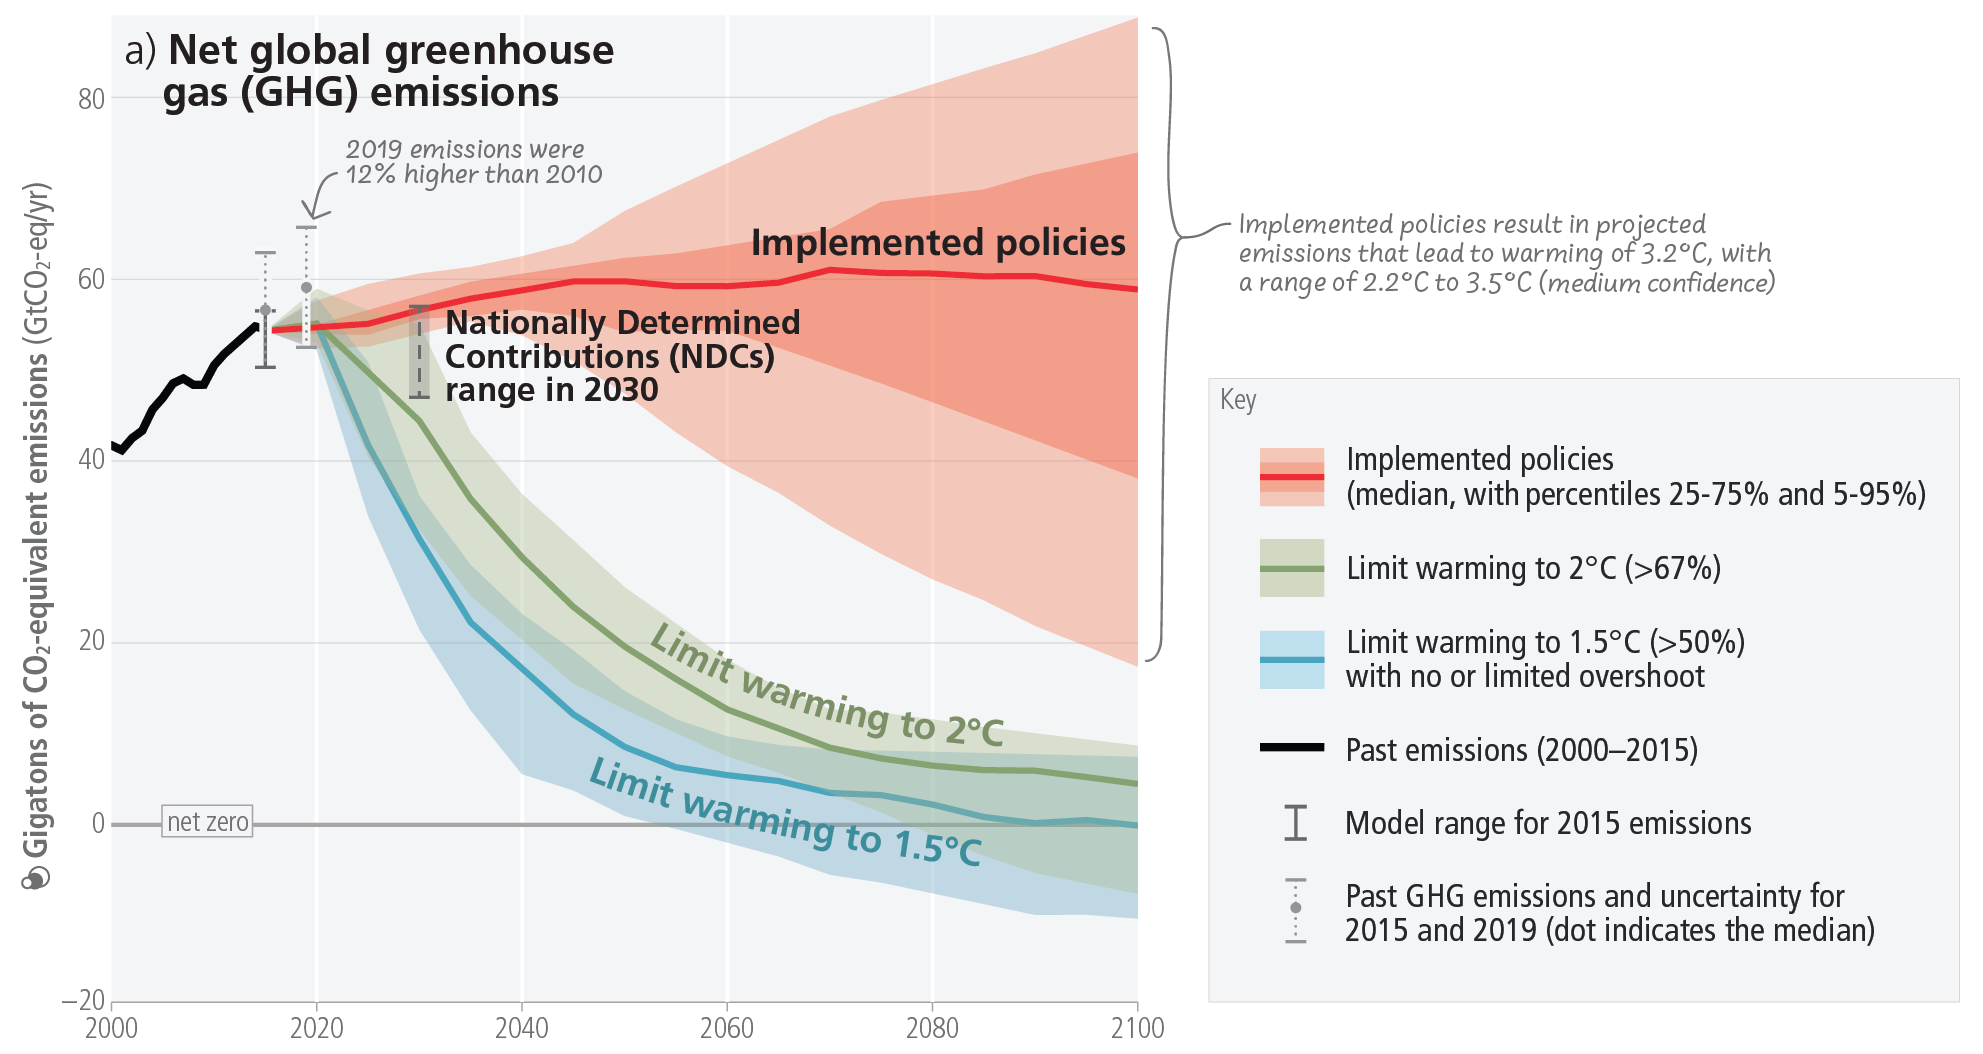
\includegraphics[width=\textwidth]{Intro/IPCC-GHG-Projection.png}
    \caption[Necessary reduction in global emissions]%
        {According to the IPCC, the global net \CdO\ emissions have to come down to zero to limit global warming. To avoid irreversible tipping points, mitigation pathways should limit warming to 1.5\degree C, which requires deep, rapid and sustained emissions reductions.  Pledged policy changes announced up until October 2021 by nations party to the Paris Climate Agreement are insufficient to meet this goal.  Figure excerpted from the IPCC 2023 Synthesis Report, Ref. \cite{IPCC2023SynthesisSPM}.
        \label{fig:ene-netco2}}
    \end{figure}
%%%%%


\begin{figure}
    \centering
    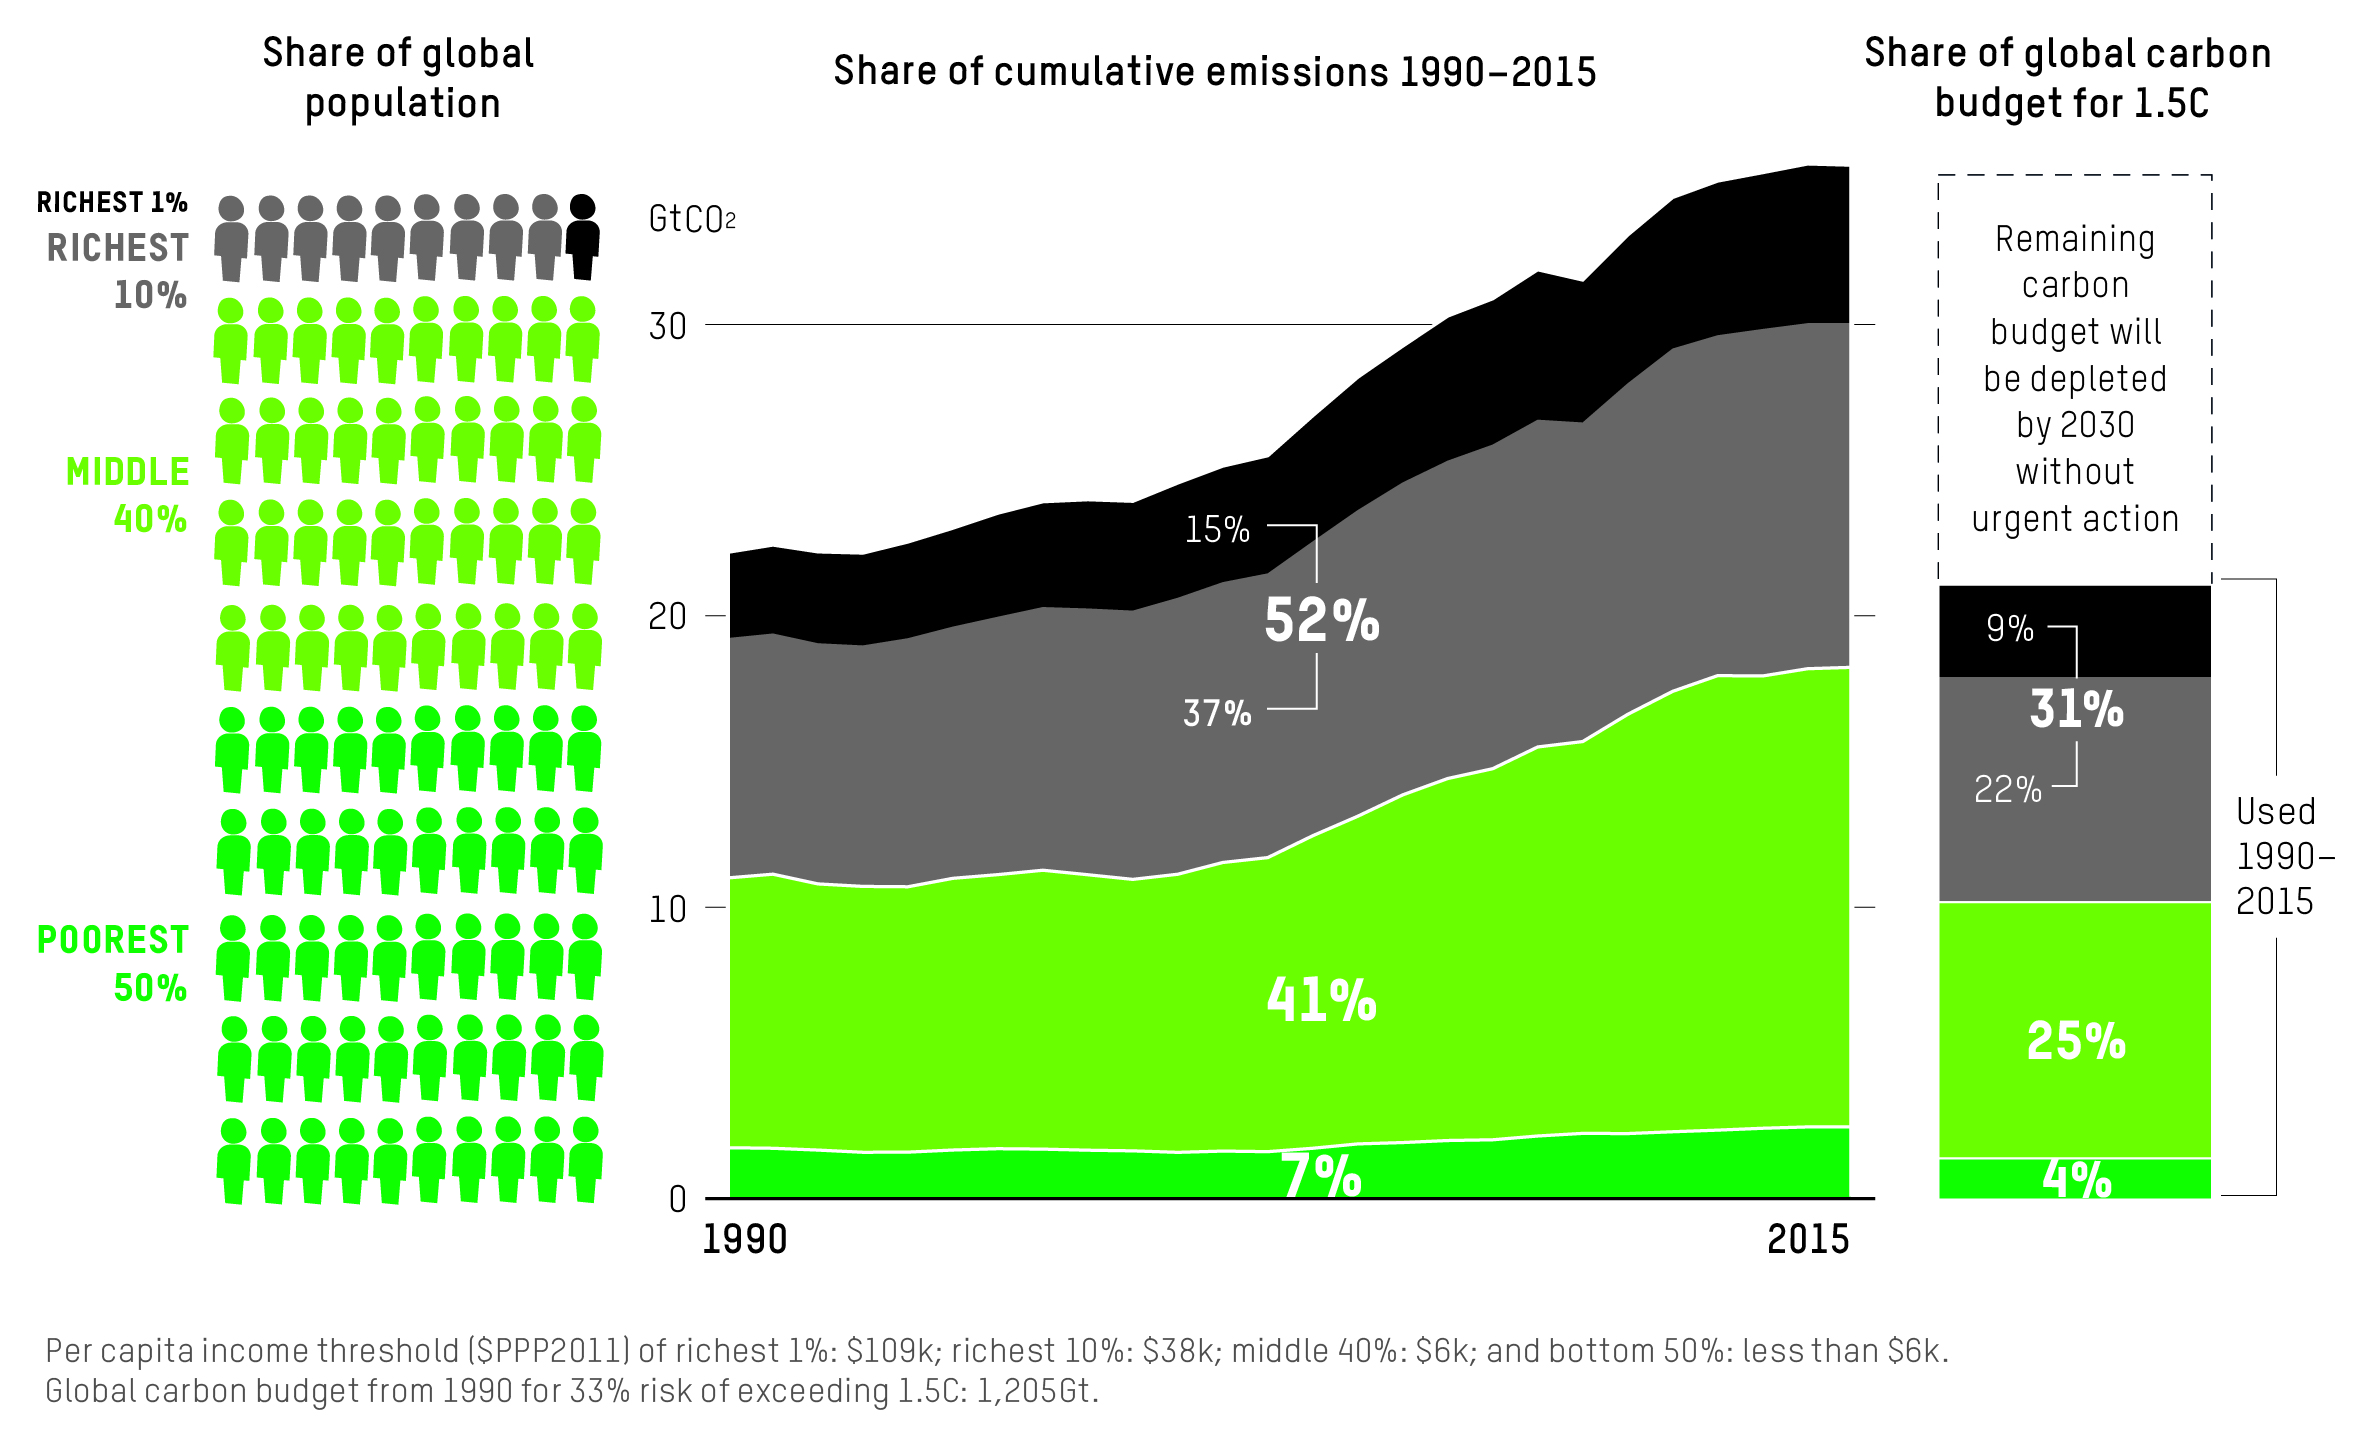
\includegraphics[width=\textwidth]{Intro/OxfamFig.jpg}
    \caption[Global emissions (1990--2015) by income groups]{Share of cumulative emissions from 1990 to 2015 and use of the global carbon budget for 1.5\degree C linked to consumption by different global income groups. Figure reproduced from Ref.~\cite{Oxfam2020} with the permission of Oxfam.\footnote{Oxfam House, John Smith Drive, Cowley, Oxford OX4 2JY, UK, \url{https://www.oxfam.org.uk/}.  Oxfam does not necessarily endorse any text or activities that accompany the materials.}}
    \label{fig:OxfamFig}
\end{figure}

Oxfam's recent publication "Confronting carbon inequality"~\cite{Oxfam2020} notes a strong correlation between GHG emissions and income level, with the world's wealthiest 10\% accounting for over half of cumulative global emissions (see \fref{fig:OxfamFig} for infographic). This income bracket, corresponding to an average annual income of over \euro{34,000}, includes many \ACR\ physicists, and was identified by the IPCC as having ``the greatest potential for emissions reductions, \eg as citizens, investors, consumers, role models, and professionals''~\cite{IPCC2022reportSPM}.  See Inset~\ref{personal} for a summary of individual climate actions ranked by impact, based on Ref.~\cite{Wynes_2017}. 


\fref{fig:intro-GlobalEmissions} presents a breakdown of 2016 global GHG emissions by sector, with the emissions at the European Organization for Nuclear Research (\acrshort{cern}) for 2019, during the Large Hadron Collider (\acrshort{lhc}) shutdown, shown as a proxy for research emissions.\footnote{Note that direct and indirect emissions more than double when the LHC is operational \cite{Environment:2737239}.}  CERN, like other \ACR\ institutions, categorises its emissions by scope rather than sector, making a direct comparison difficult.  Instead, we consider total
per-capita emissions, dividing CERN's emissions equally amongst its seventeen thousand Users (scientists involved in CERN-based research), to obtain roughly 15 \acrshort{tco2e} per researcher per annum, or twice the global average of 6.3 \acrshort{tco2e}.  Note that this does not include personal household emissions for researchers, which may exceed their workplace emissions.  It also incorrectly assigns some emissions due to CERN's smaller cohort of direct personnel, \eg due to CERN-funded travel or personal computing equipment, to its entire User base.  
%
%%%%%
\begin{figure}[!tb]
    \centering
    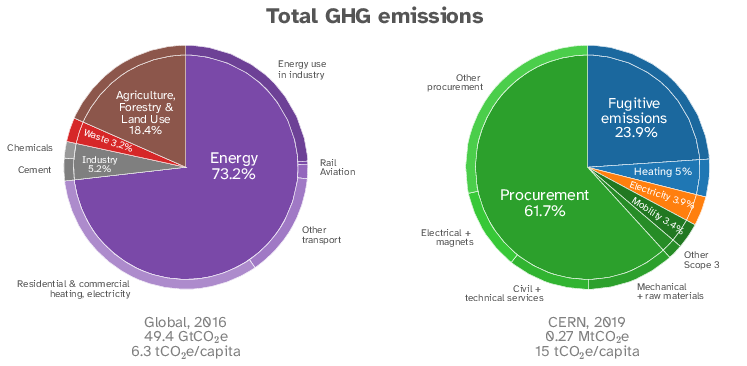
\includegraphics[width=0.98\linewidth]{Intro/GlobalEmissions.png}
    \caption[2016 global GHG emissions vs 2019 CERN emissions]%
        {Distribution of 2016 global GHG emissions by sector, compared with CERN emissions for 2019, during LHC shutdown. Data are taken from Ref.~\cite{OWIDGHGSector} and CERN Environmental Reports~\cite{Environment:2737239,CERN:2723123,Hartley}. \label{fig:intro-GlobalEmissions}}
    \end{figure}
%%%%%
%
For a fairer accounting, see \fref{fig:Intro-ComparativeEmissions}.  This chart attributes reported work-related emissions in each sector to the `true' consumers of each resource, for researchers at CERN as well as four other \ACR\ institutions, the Max Planck Institute for Astronomy (\acrshort{mpia}) in Heidelberg, Germany, the Department of Physics (\acrshort{dphys}) at \acrshort{eth}, \acrshort{nikhef} in the Netherlands, and Fermilab in Chicago, USA (\acrshort{fnal}).  For raw data and details of underlying methodology, see Appendix~\ref{sec:DataforFig1.4}.  Note that these institutions are somewhat self-selected, counting among the minority that have published quantitative estimates of their environmental footprint.  Since CERN is the only institution on this list that attempts a full accounting of its Scope 3 emissions, the numbers in this chart should be taken as indicative only, and caution should be employed in making comparisons across institutions on this basis.\footnote{CERN procurement data were estimated with a spend-based method~\cite{SpendBased} using the ecoinvent database~\cite{ecoinvent}. The results therefore have a large margin of error and should be interpreted with care.}   It is nevertheless evident that work-related emissions for many of HECAP+ researchers far exceed our remaining budget to stay within 
1.5\degree C of warming~\cite{IPCC2021reportSPM}.\footnote{The per-capita budget is computed using an emissions budget of 420 G\tCdOe\, and an average world population of 8.8 billion.} 

\begin{figure}[!tb]
    \centering
    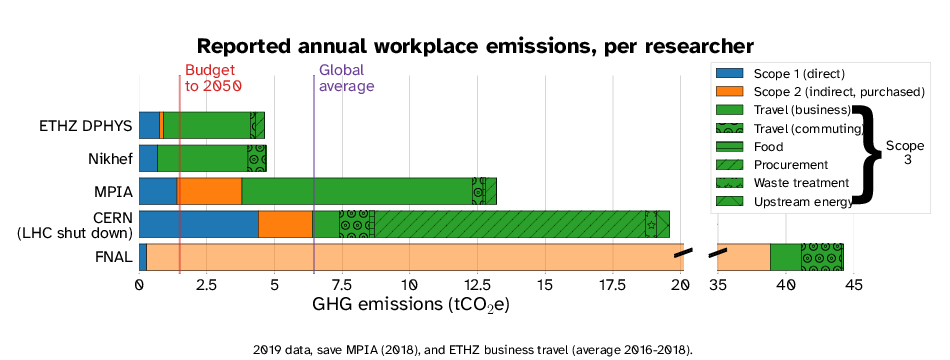
\includegraphics[width=\textwidth]{Intro/ComparativeEmissions.png}
    \caption[Reported workplace GHG emissions for researchers at \ACR\ institutions]{Reported workplace GHG emissions, distributed among researchers at five different \ACR\ institutions, with the global per-capita average, and remaining carbon "budget" to stay within the Paris Climate Accord limit of 1.5\degree C of warming shown for comparison.
    CERN data for 2019 is taken from Ref.~\cite{Environment:2737239,CERN-HR-STAFF-STAT-2019,CERN:2723123,Hartley}, MPIA data for 2019 from Ref.~\cite{Jahnke2020}, ETHZ DPhys data from 2018 taken from Ref.~\cite{Beisert2020}, Nikhef data from 2019 from Ref.~\cite{Nikhef}, and Fermilab (FNAL) data from Ref.~\cite{FermilabEnvReport2019}. Scope 3 estimates are incomplete for all but CERN.  To estimate emissions per researcher, each individual emissions category was divided by the nominal number of users for that resource, see Appendix~\ref{sec:DataforFig1.4} for details.  
    \label{fig:Intro-ComparativeEmissions}}
\end{figure}

These work-related emissions are due to choices we make, as individuals, collaborations, or institutions.  They could be a direct consequence of \ACR\ research, such as the choice of detector design; computing setup or software pipeline for simulation and analysis; or how we collaborate or communicate the results of our work.  Alternatively they could be peripherally related to the science we do:~e.g., how we commute between our home and workplace, or the food we consume while at work; or how our offices are powered, heated and ventilated. 
Historically, many of these choices have been made prioritising cost or convenience over environmental and social impact.  However, the rapid and systemic societal change needed to keep to our climate change goals requires system-wide engagement at all levels of academia.  We can impel positive change throughout the academic research system by re-assessing these choices and how central they are to our primary function as scientists.

This process has already begun. Universities and other institutions are including sustainability in buildings planning (see \bpref{BP:Nikhef}) and engaging with voluntary assessments of the environmental sustainability of their research facilities (see \eg~Refs.~\cite{Environment:2737239, Jahnke2020, Beisert2020, Nikhef, FermilabEnvReport2019}). Examples focussed on the environmental sustainability of laboratories include France's Labos1point5 (see \bpref{BP:l1p5}) and University College London’s Laboratory Efficiency Assessment Framework (LEAF) initiative~\cite{LEAF_framework, LEAF_take_part}, a standard being adopted across an increasing number of universities~\cite{LEAF_impact}. The LEAF initiative, which awards three levels of certification to participating laboratories, is structured around online tools that promote best practice, and aid calculations of impact and reporting, as well as additional resources and training opportunities for staff and students. 

%%%%%

\begin{bestpractice}[Nikhef renovation and sustainability plan\label{BP:Nikhef}]{Nikhef renovation and sustainability plan}%
    Nikhef is the Dutch National Institute for Subatomic Physics in the Netherlands. It is both a consortium of universities and an institution with a building in Amsterdam. The total \tCdOe\ footprint of Nikhef was 1,082 \tCdOe\ in 2019,\footnote{We report the 2019 numbers, since the 2020 numbers may be unrepresentative due to the impact of the COVID-19 pandemic.} three quarters of which is due to flying to conferences and laboratories, and 15\% is due to heating the building with natural gas~\cite{Nikhef}. The building is undergoing a major renovation in 2021--2023, which will remove the need for gas for heating. Instead, the heat from the nearby data centre will be used, in addition to better thermal insulation of the building.

    The Nikhef sustainability roadmap~\cite{Nikhef} covers all sources of direct and indirect carbon emissions. For instance, by 2030, air travel should be reduced by 50\% and daily commuting should be climate-neutral.  Intermediate targets for 2025 are also set and yearly emissions will be monitored and reported.
\end{bestpractice}

%%%%%


\pagebreak

\begin{inset}[Personal emissions\label{personal}]{Personal emissions}%
\begin{figure}
    \captionsetup{type=figure}
    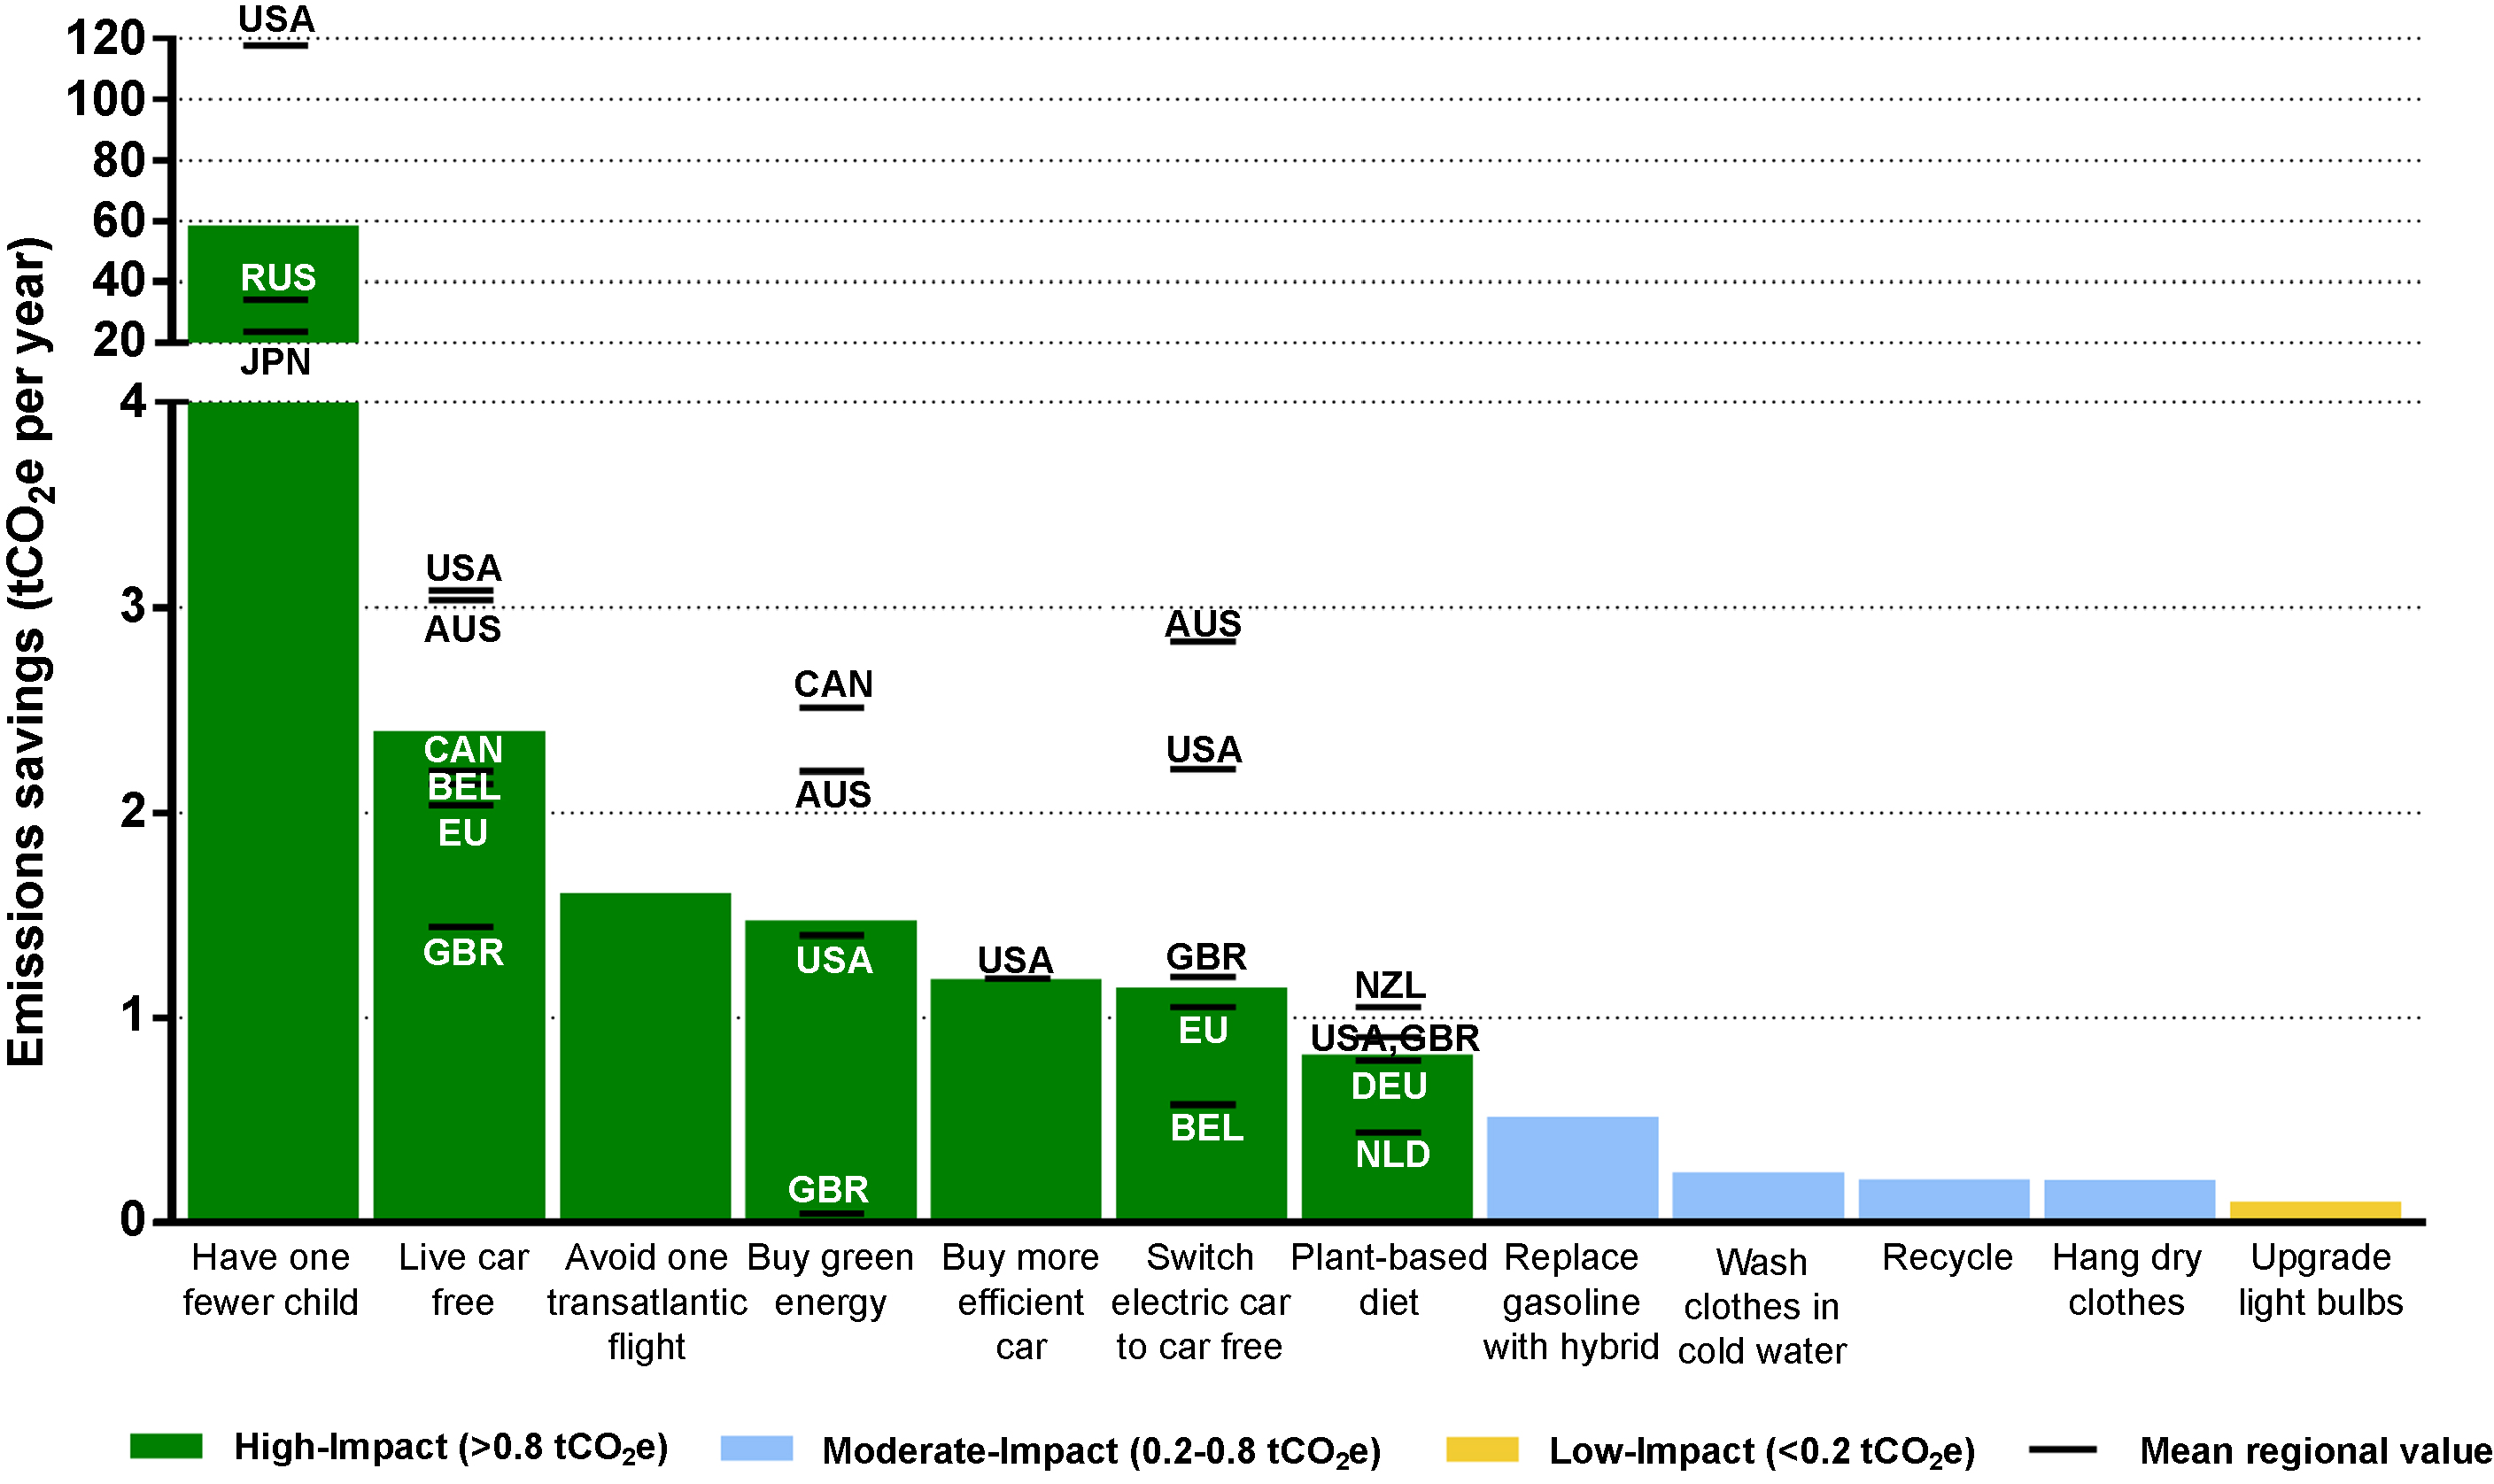
\includegraphics[width=\textwidth]{Intro/fourchoices-scientific.jpg}
    \caption[Emissions reduction from individual actions]{Emissions reduction from individual actions.  Black lines correspond to individual developed nations studied, the mean over which is shown as a coloured bar.  Note that these numbers are based on average current emissions in developed countries, neglecting the effects of climate policy.  The break in the left-most bar distinguishes between the emissions due to direct offspring and integrated emissions over all generations of descendants.  Moreover, the integrated estimate assumes emissions per capita that are constant in time. See the accompanying text and footnote for a more detailed exposition of the underlying assumptions and leading systematic uncertainties. Figure reused from Ref.~\cite{Wynes_2017} under the terms of the \href{https://creativecommons.org/licenses/by/3.0/}{Creative Commons Attribution 3.0 Unported (CC-BY 3.0) License}.}
    \label{fig:Intro-EffectiveEmissionsReduction}
\end{figure} 
Figure~\ref{fig:Intro-EffectiveEmissionsReduction} shows the conclusions of a recent meta-study from Lund University~\cite{Wynes_2017}, in which individual climate actions were ordered by impact.  Note that the authors assume ``average conditions in developed countries'', so miss the substantial differences between emissions levels in developing and developed nations.  They also neglect the effects of climate policy.  For one estimate of how national climate policies might modify the ordering, see Ref.~\cite{FoundersPledge}. This figure highlights the disconnect between the moderate-impact measures (right-most five bars) that consumers are commonly encouraged to take, and the high-impact measures (left-most seven bars) that pertain to more complex and nuanced issues.\footnote{The left-most bar, the climate cost of having an additional child, relies on the assumption that global emissions per capita remain frozen at their 2005 value.  The 2009 study from which this estimate was taken~\cite{MURTAUGH200914} also quotes results assuming two alternative
emissions scenarios considered in the 2007 IPCC report:~an `optimistic' scenario, in which emissions per capita decrease linearly to 0.5 \tCdOe\ by 2100, and a `pessimistic' one, in which they increase linearly to 150\% of their 2005 value of 4.3 \tCdOe.  The systematic uncertainty in the result due to this choice is huge, with the estimated cost of having an additional child ranging from 4.6 \tCdOe\ in the optimistic scenario, to 81 \tCdOe\ in the pessimistic one.  The lower and upper limits of this range were obtained by dividing the lifetime emissions per child in each case by the average human lifespan, as reported in Ref.~\cite{UN2019}, in the developed country in question.
This still raises the question of how responsibility for the emissions of future generations should be allocated, given that children are essential to the functioning of our society and institutions.}
A full discussion of these issues is beyond the scope of this document.
\end{inset}

%%%%%%%%%%%%%%%%%%%%%%%%%%%%%%%%%%%%%%%%%%%%%%%%%%

\newpage

\subsection{Previous and Parallel Initiatives}
\label{sec:other_initiatives}

This document is focused on environmental sustainability and associated social justice issues of particular relevance to the activities of \ACR. It is important to acknowledge the attention that these topics are rightly being given across our communities. This includes, e.g., in conference plenary talks and in parallel tracks devoted to sustainability, and equity, equality, diversity, inclusivity and accessibility. This section provides a brief review of other documents with similar and complementary focuses on environmental and wider social responsibilities.

%%%%%%%%%%%%%%%%%%%%%%%%%%%%%%%%%%%%%%%%%%%%%%%%%%

\subsubsection{ALLEA, Towards Climate Sustainability of the Academic System in Europe and Beyond}

The All European Academies (ALLEA) Working Group on Climate Sustainability in the Academic System published a report in May 2022~\cite{ALLEA}, the aim of which is "to  assess current practices and to critically examine current and proposed measures." 
The document urges stakeholders --- either individual (researchers and students) or structural (universities, funding bodies, conference organisers, ranking agencies, and
policy makers) --- to know their roles and responsibilities toward a climate-sustainable academic system.
After summarizing available data on GHG emissions from various stakeholders and reviewing
the current practices aimed at reducing those
emissions, the report outlines recommendations for individual and group stakeholders. 
Dimensions of social justice and equity are among the principles underlying all recommendations, as well as the opportunity for the academic system to be a role model in the matter. 
While all group stakeholders are advised to embed sustainability in their strategies, individual ones differ:\ students and academic members are encouraged to hold university management accountable, to demand divestment and to generate awareness. 
The importance of the development of an evidence base is emphasised, along with mix-and-match approaches to meeting formats. 
Finally, stakeholders are pushed to allocate funding to the decarbonization of the academic system.

%%%%%%%%%%%%%%%%%%%%%%%%%%%%%%%%%%%%%%%%%%%%%%%%%%

\subsubsection{Snowmass Contribution, Climate Impacts of Particle Physics}

The report "Climate impacts of particle physics"~\cite{Bloom:2022gux}, submitted to the proceedings of the US Community Study on the Future of Particle Physics (Snowmass 2021) focuses on facility construction, detector gases, computing, and GHG emissions from particle physics laboratories. 
The report highlights two key motivations for addressing the ecological and climate impacts of particle physics: (i) that the particle physics community has a moral obligation to do so and (ii) that its professional activities will be under increasing scrutiny from a number of stakeholders. 
The latter means that the community will be under increasing pressure to justify its carbon emissions against its relative size, compared to other industries, and its societal benefits.

As a concrete example, the report focuses on the Future Circular Collider (FCC) --- the proposed 100 TeV electron-positron (and later hadron) collider. 
The authors estimate that the construction of the roughly 100 km circumference tunnel alone would lead to \CdO\ emissions at the level of a few hundred kilotons, several times more than other large US building projects.
This corresponds to "per physicist" emissions 80 times larger than their estimated 1.1 \acrshort{tco2}\ per capita per year limit needed to keep global warming to less that 1.5\degree C. The authors emphasise the significant impact of the GHGs used in particle physics detectors and for cooling, which can have warming potential that exceeds that of \CdO\ by as much as four orders of magnitude (in the case of ${\rm SF}_6$).  
The report then highlights a number of avenues for reducing the GHG emissions due to the electricity consumption of computing, which is pivotal to running and exploiting such facilities. It also discusses the additional emissions due to collaborative research activities, with a particular emphasis on taking careful steps to reduce air travel that capitalise on potential benefits for social justice while minimising unintended negative consequences for members of the community.

The report's recommendations stress the need for reporting on planned emissions and energy usage for new facilities; standardised reporting of emissions across the sector, and community-wide engagement to tackle the negative climate impacts of particle physics research through dedicated research time.

\subsubsection{Recommendations by the yHEP association in Germany}

The young High Energy Physicists (yHEP) association in Germany published the "yHEP recommendations on improvement of environmental sustainability in science"~\cite{yHEP1} and its Addendum~\cite{yHEP2} in December 2020 and 2021, respectively. The documents, which were the result of proposals from the yHEP community, including HECAP, hadron and nuclear, and accelerator physicists, contain ideas for improving the environmental sustainability of basic research. They take a qualitative approach on a broad range of topics, including, but not limited to, travel, conferences, computing and infrastructure, resource management and financing, and green energy. 

%%%%%%%%%%%%%%%%%%%%%%%%%%%%%%%%%%%%%%%%%%%%%%%%%%

\subsection{Impelling Positive Change}

The aim of this document is to provide as comprehensive a discussion as practicable of the various impacts of \ACR\ research, from our day-to-day activities through to the large infrastructure projects on which our science depends. The discussions presented here have much in common with those of the documents described in \sref{sec:other_initiatives}. This document is, however, intended to have broad scope and, through case studies and best practice, to illustrate potential actions that can be implemented at individual, group and institutional levels to limit the impacts of \ACR\ research on the world's climate and ecosystems.

However, if the \ACR\ community is to succeed in improving the sustainability of its working practices, then the environment and related issues of social justice must be recognised as integral parts of the planning and management of our research activities. With this in mind, we collect below a list of recommendations for structural changes to the organisation of our community, our training and our professional development.

These recommendations complement those listed in the discussions of specific sources of environmental impacts of \ACR\ research on which the bulk of this document focuses. Together, these provide concrete suggestions of ways in which the \ACR\ community can act to reduce its negative climate and ecological impacts, and address issues of social justice in line with the United Nations Sustainability Goals, discussed in the next subsection.

%%%%%%%%%%%%%%%%%%%%%%%%%%%%%%%%%%%%%%%%%%%%%%%%%%

\clearpage
\begin{minipage}{\textwidth}
\begin{reco2}{\currentname}
{
\begin{itemize}[leftmargin=6 mm]
\setlength\itemsep{\recskip}
\item Consider the environmental impact of work practices.

\item Be proactive in seeking best practice.

\item Make and model positive change in research activities.

\item Drive positive group and institutional actions.
\end{itemize}
}
{
\begin{itemize}[leftmargin=6 mm]
\setlength\itemsep{\recskip}
\item  Include critical assessment of the environmental impact of all activities during planning stages.

\item  Monitor, assess, report on and set targets in relation to the environmental impacts of research activities.

\item Drive institutional actions, and encourage, support and incentivise individual actions, e.g., through training.

\end{itemize}
}
{
\begin{itemize}[leftmargin=6 mm]
\setlength\itemsep{\recskip}
\item Require funding applications to outline plans for monitoring, reporting and minimising adverse environmental impacts, and for ensuring that research is undertaken in line with principles of social justice.

\item Allow flexibility in policies and procedures \eg budget allocation, that enable environmentally sustainable choices to be made.

\item Ensure that degree programmes include a focus on global citizenship, encompassing environmental sustainability and associated social justice implications.

\item Acknowledge focus on environmental sustainability and social justice in the accreditation of degrees by governments and professional bodies.

\item Encourage, support and incentivise individual and group actions, \eg by considering them in professional development and appraisal processes.

\end{itemize}
}

\end{reco2}
\end{minipage}

%%%%%%%%%%%%%%%%%%%%%%%%%%%%%%%%%%%%%%%%%%%%%%%%%%

\newpage
\subsection{United Nations Sustainable Development Goals}

%%%%%

\begin{figure}[!ht]
     \centering
     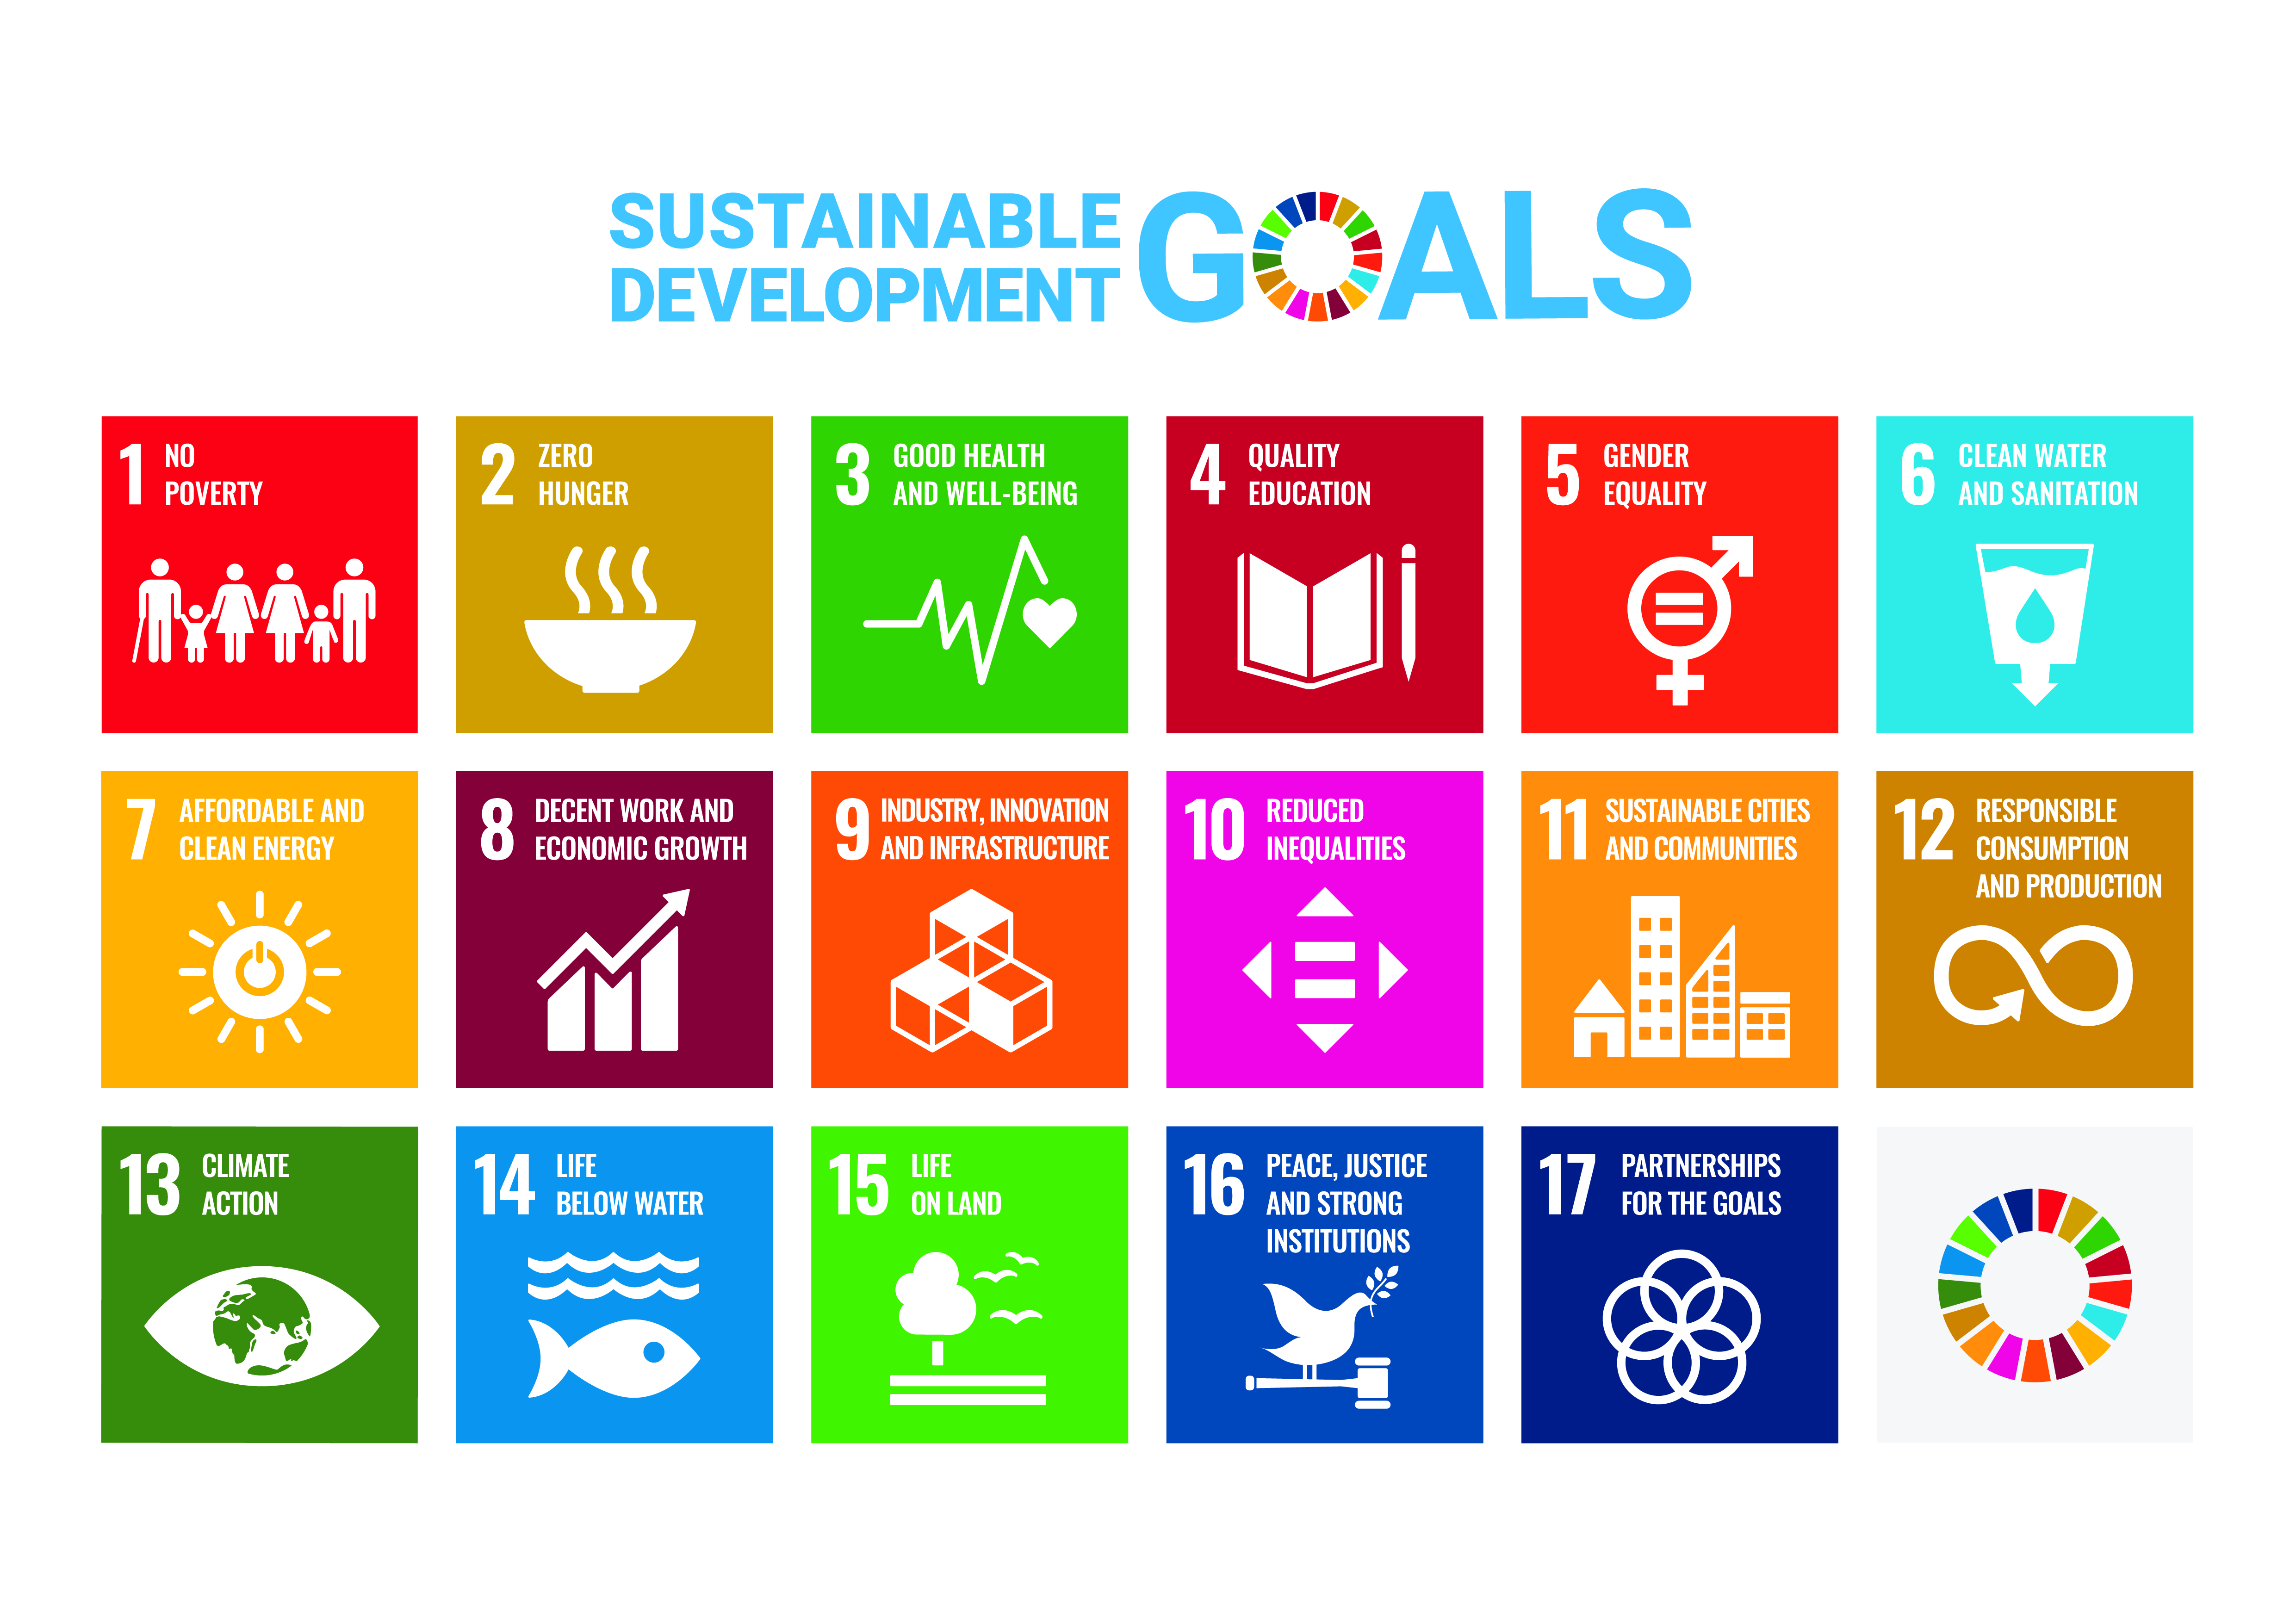
\includegraphics[width=0.75\linewidth]{Intro/ESDG_Poster2019_PRINT.jpg}
     \caption[United Nations Sustainable Development Goals]{The seventeen United Nations Sustainable Development Goals~\cite{UNSustainableGoalsFigure}.\label{fig:17_UN_SustGoals}}
\end{figure}

%%%%%

As a global research community, \ACR\ has an impact on society all over the world. We contribute to basic scientific knowledge, drive innovation and promote international collaboration. Our institutions are large employers, large consumers of goods and services, and a key resource in the training and development of national skills bases. This places our institutions in a position to influence policy decisions, drive investment in local infrastructure, and leverage wider improvements to social and environmental standards. For these reasons, the \ACR\ community is in a strong position to support the UN Sustainable Development Goals (SDGs), summarised in~\fref{fig:17_UN_SustGoals}.

The topics discussed in this document are meant to support a multiplicity of these goals, and we aim to signpost the influence of our work in all aspects. The goals are listed below, with examples of how each is impacted by the HECAP+ research community and its work. The SDGs are defined in UN resolution A/RES/70/1 in detail~\cite{UNResolutionARES701}. It is impossible to cover all aspects in this document, but the manifold impact of the \ACR\ community on sustainable development is clear from this non-exhaustive list. 

\bigskip

%%%%%%%%%%%%%%%%%%%%%%%%%%%%%%%%%%%%%%%%%%%%%%%%%%

\newcommand{\SDGscale}{0.05}
\newcommand{\iconskip}{-2em}
\newcommand{\SDGleft}{0.07}
\newcommand{\SDGright}{0.89}
\renewcommand*{\arraystretch}{3}
\noindent\begin{longtable*}{l l}
\parbox[t]{\SDGleft\textwidth}{\raisebox{\iconskip}{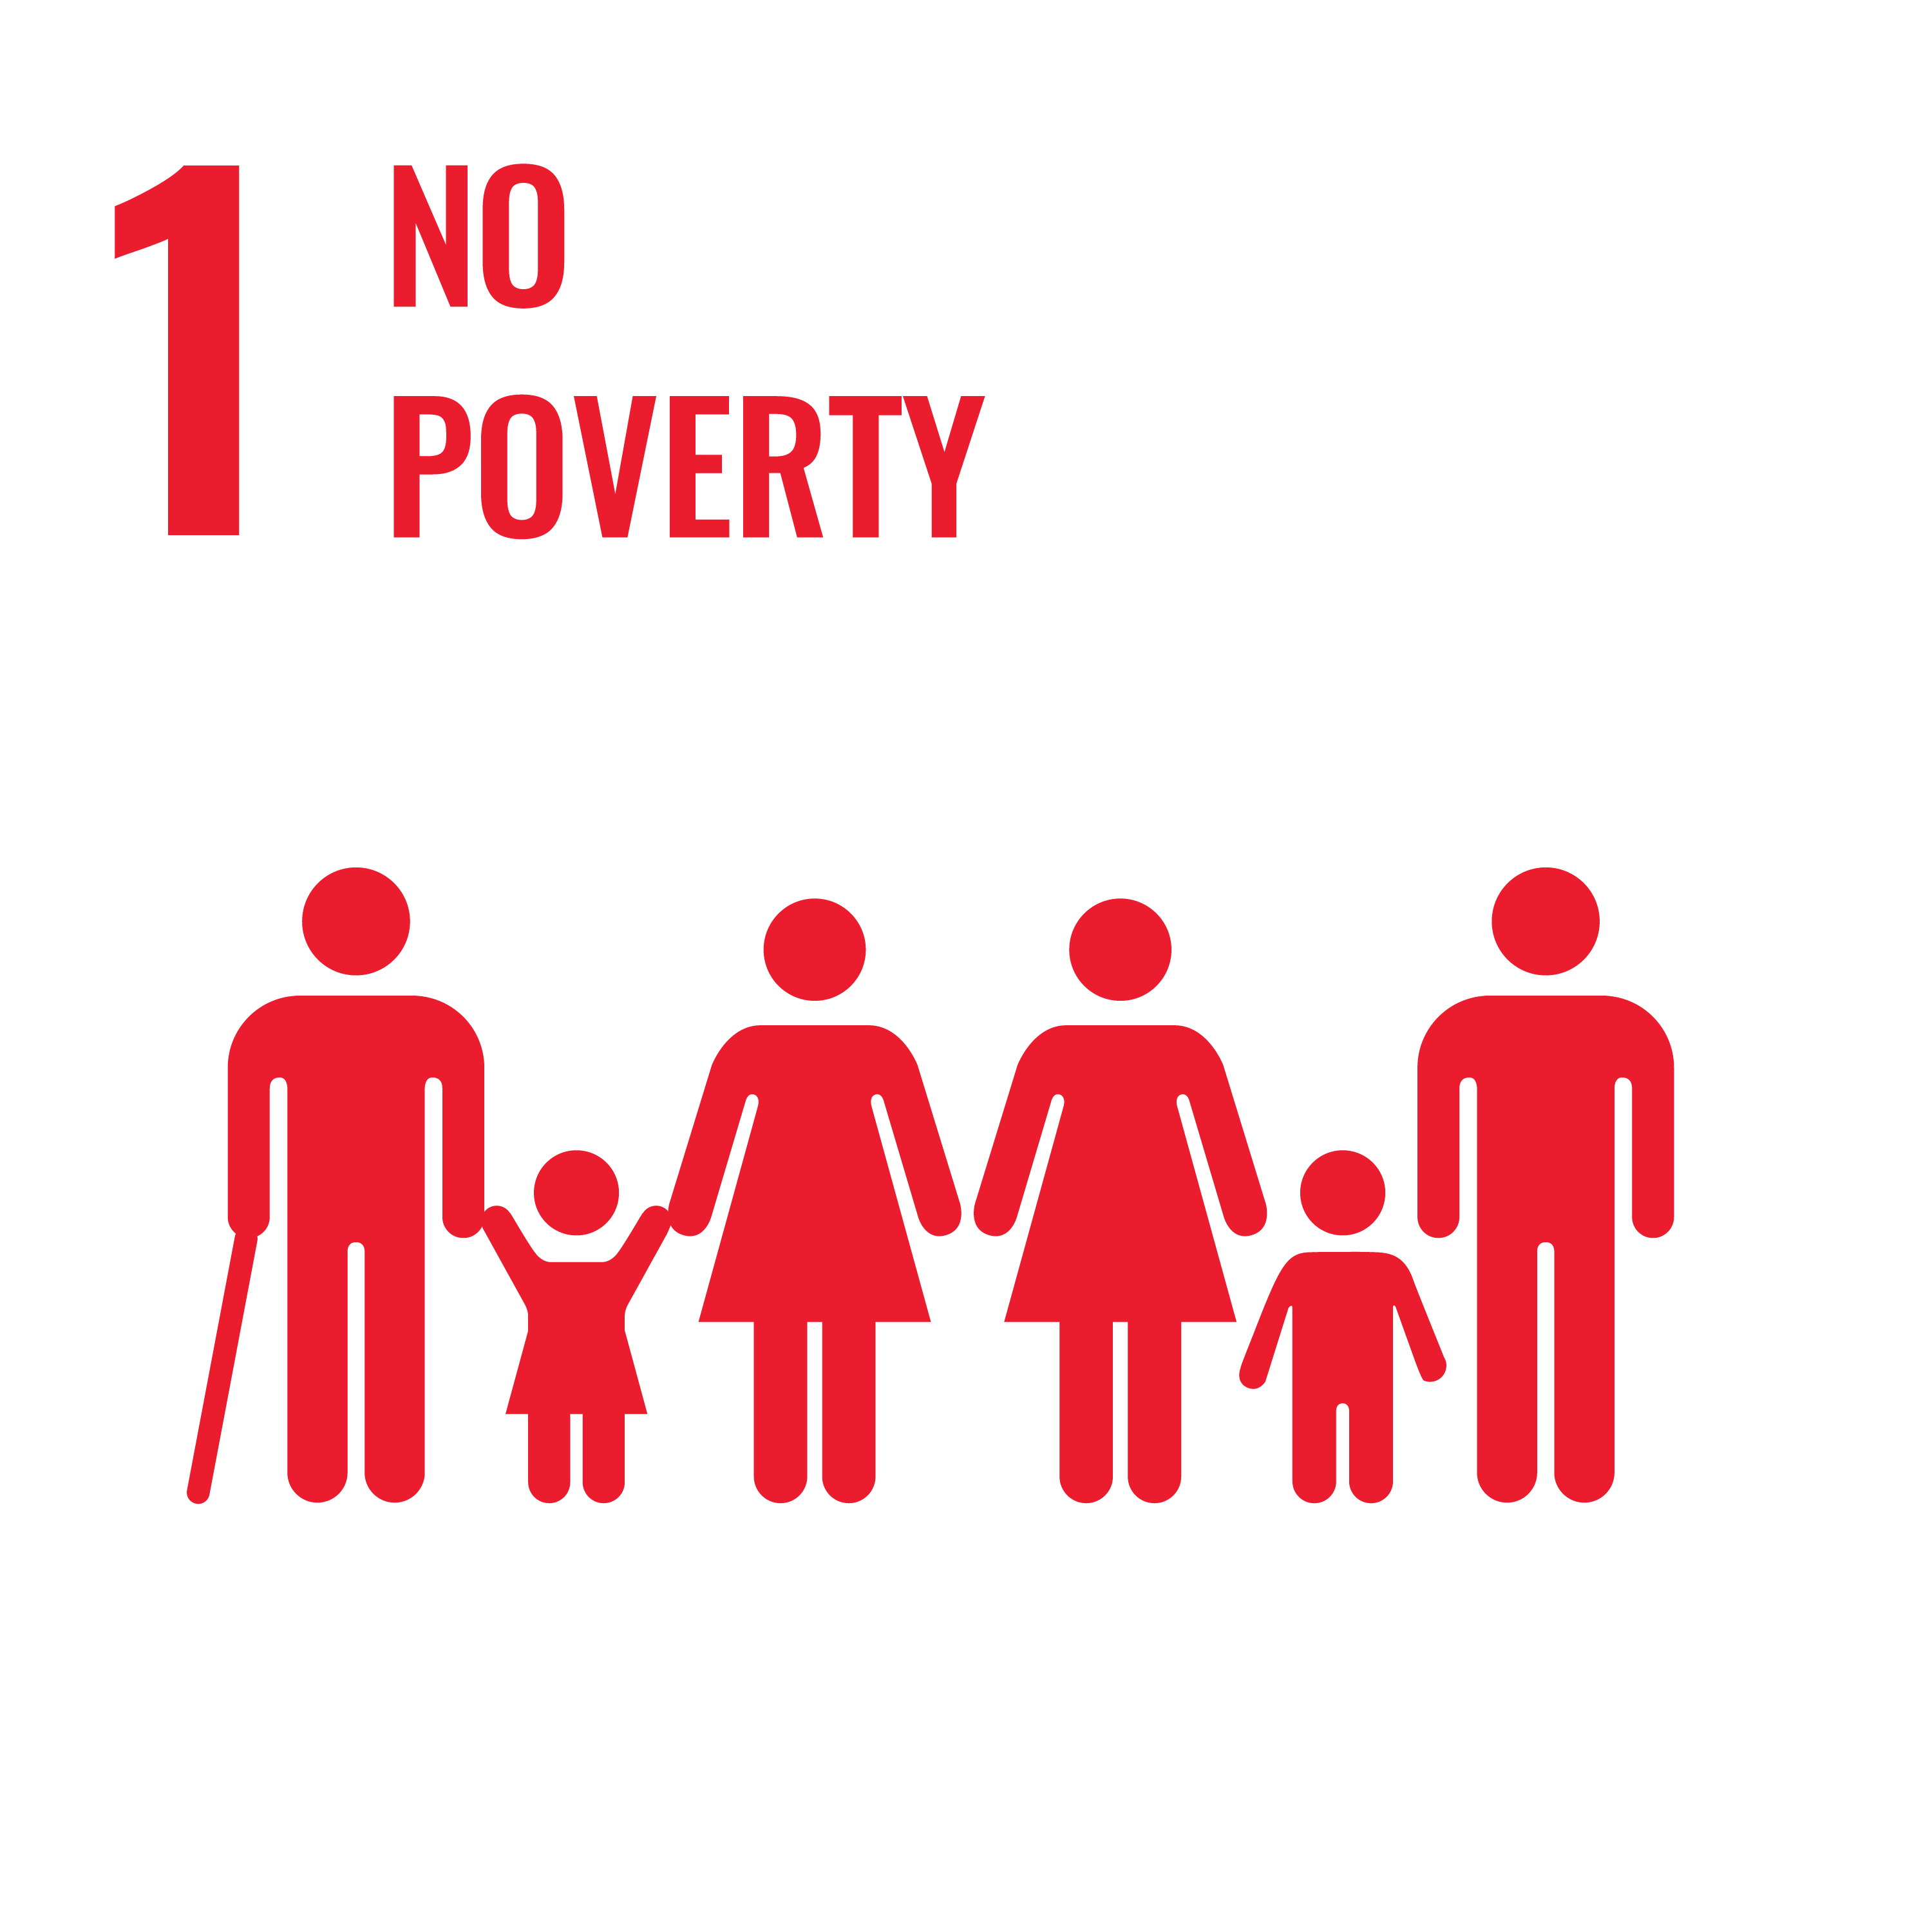
\includegraphics[scale=\SDGscale]{Sections/Figs/Common/SDG_1_NoPoverty.png}}} & \parbox[t]{\SDGright\textwidth}{\textbf{Goal 1:\ No poverty --- End poverty in all its forms everywhere}
\vspace{\recskip}
\begin{itemize}[leftmargin=20pt]
\setlength{\itemsep}{\recskip}
\item The contractual and payment standards in employment contracts of institutes and collaborations influence their employees' lives.
\item The terms of contract with external companies influence the working and living conditions of their employees.
\end{itemize}}\\
\parbox[t]{\SDGleft\textwidth}{\raisebox{\iconskip}{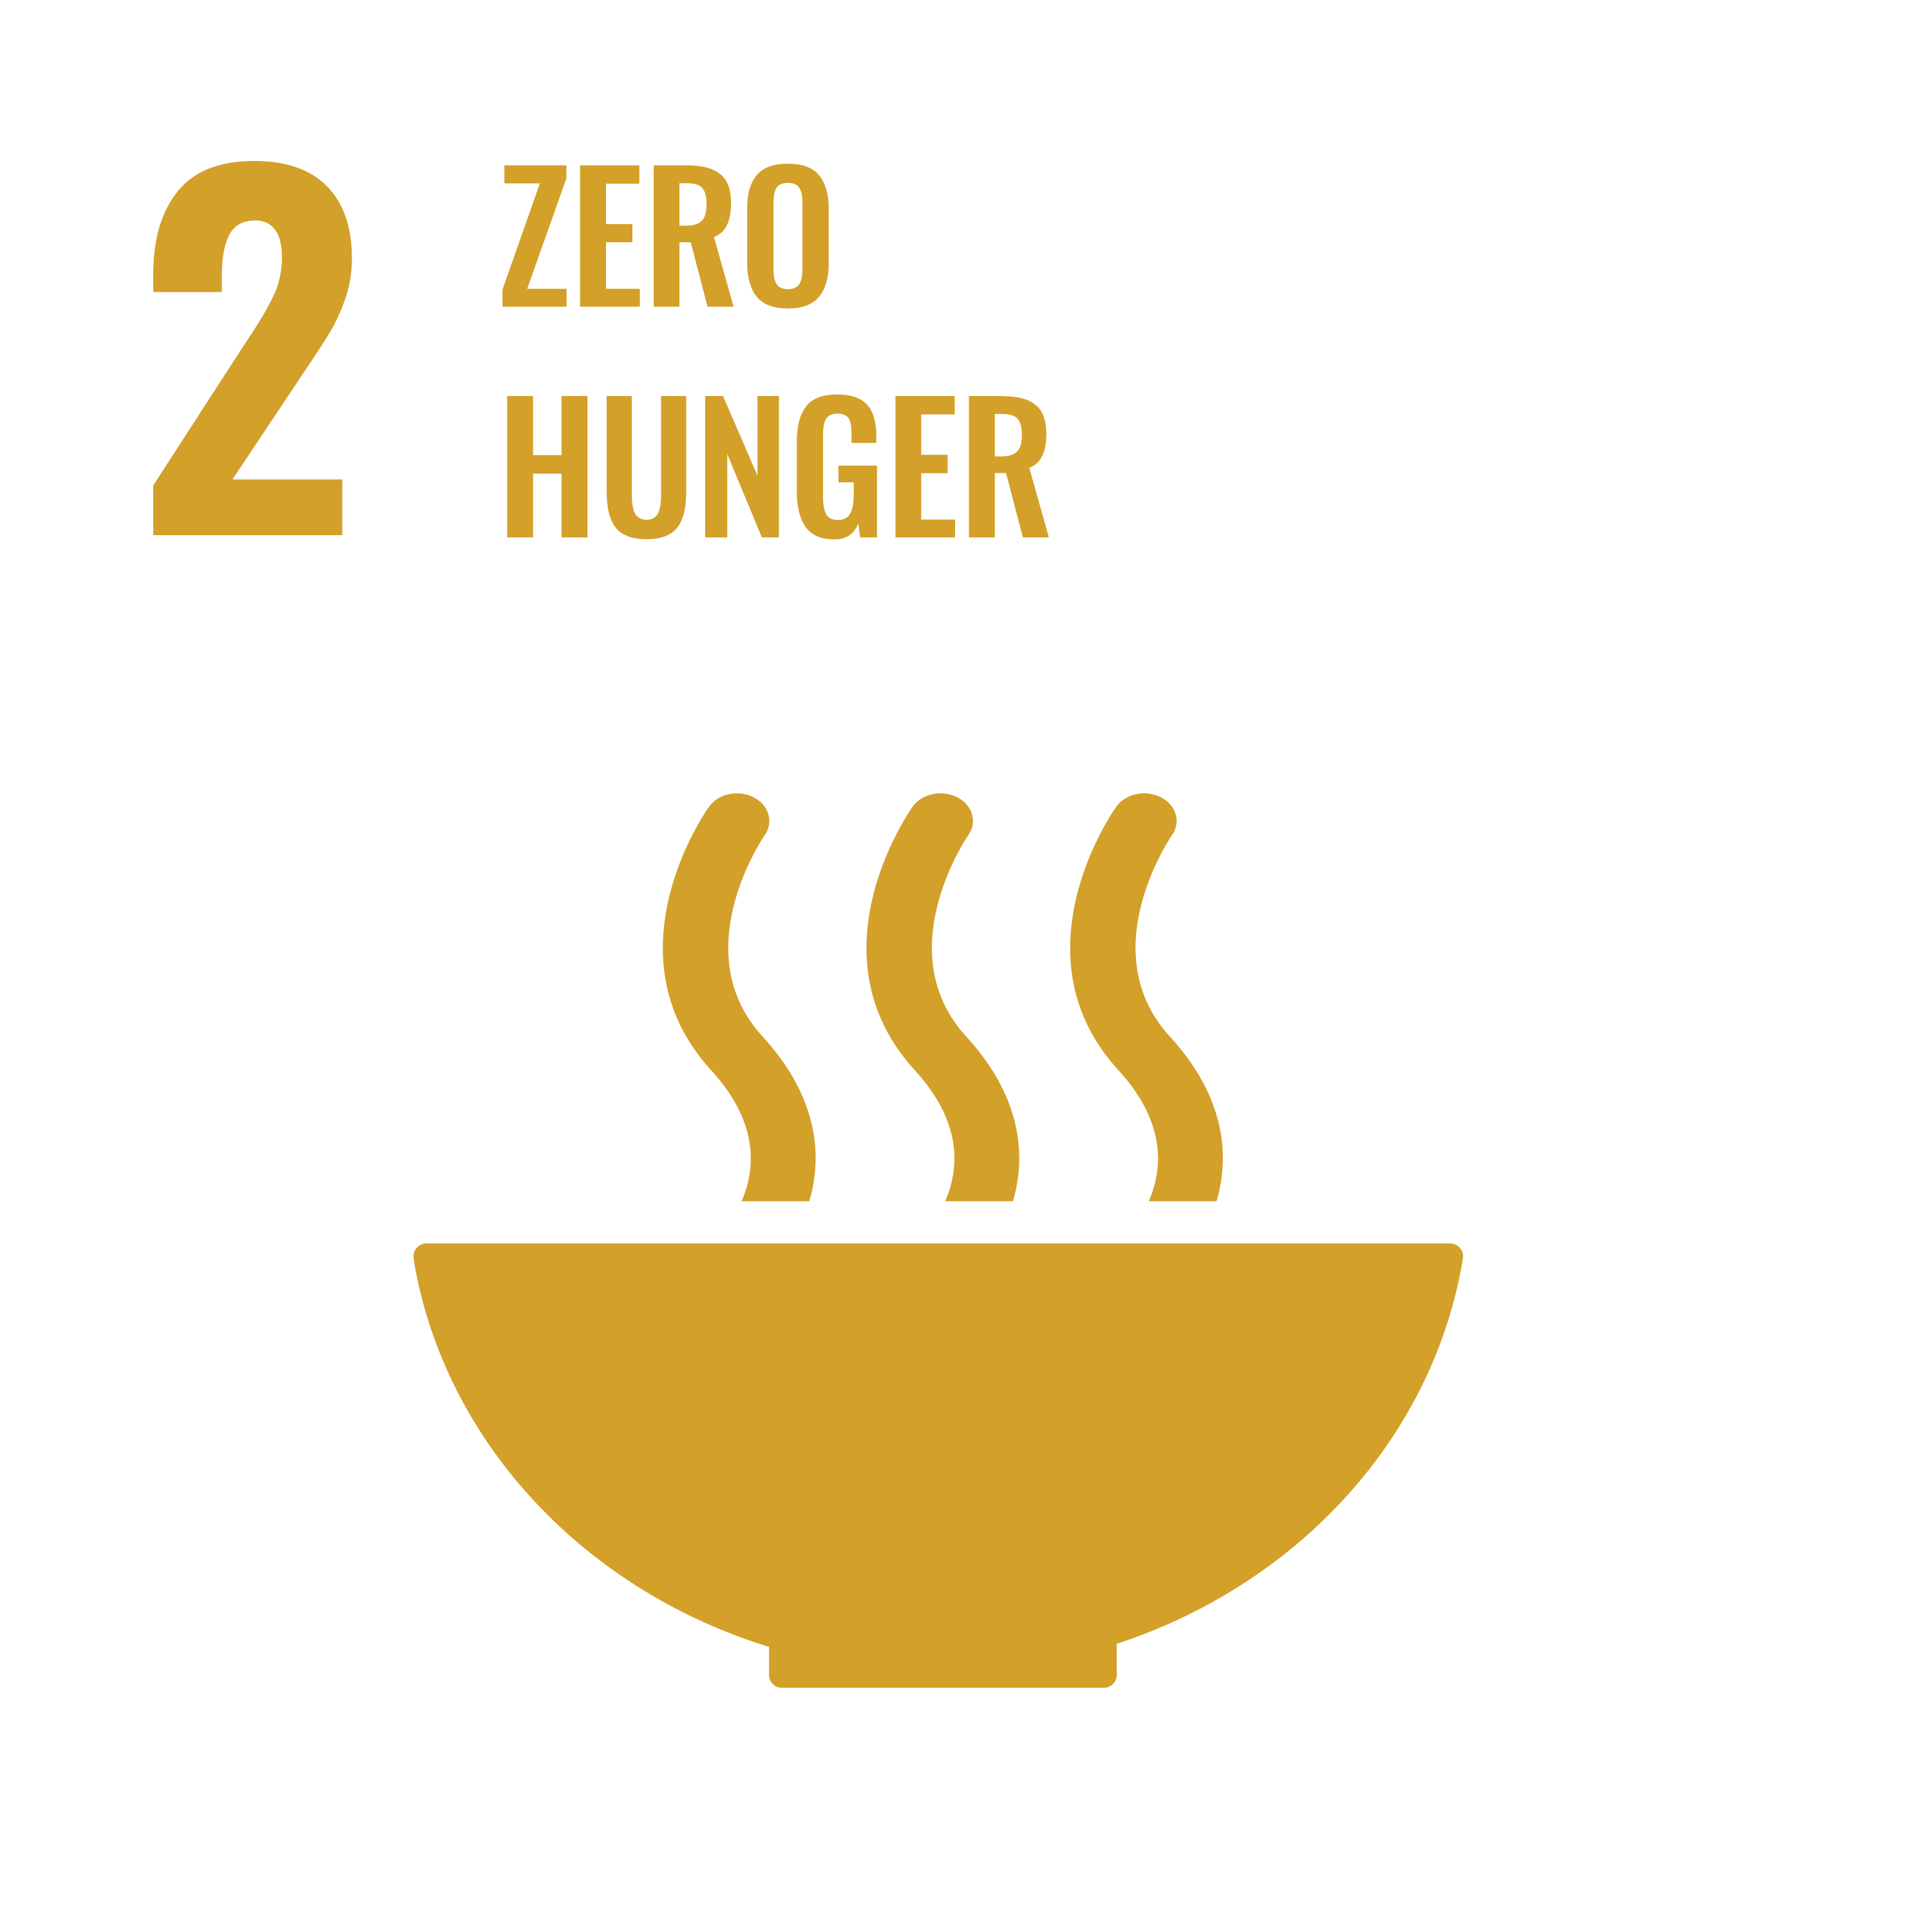
\includegraphics[scale=\SDGscale]{Sections/Figs/Common/SDG_2_ZeroHunger.png}}} & \parbox[t]{\SDGright\textwidth}{\textbf{2 Zero hunger:\ End hunger, achieve food security and improved nutrition and promote sustainable agriculture}
\vspace{\recskip}
\begin{itemize}[leftmargin=20pt]
\setlength{\itemsep}{\recskip}
\item The food consumed at institutes and events has an effect on the behaviour of the food market/industry from which it is purchased.
\end{itemize}}\\

\parbox[t]{\SDGleft\textwidth}{\raisebox{\iconskip}{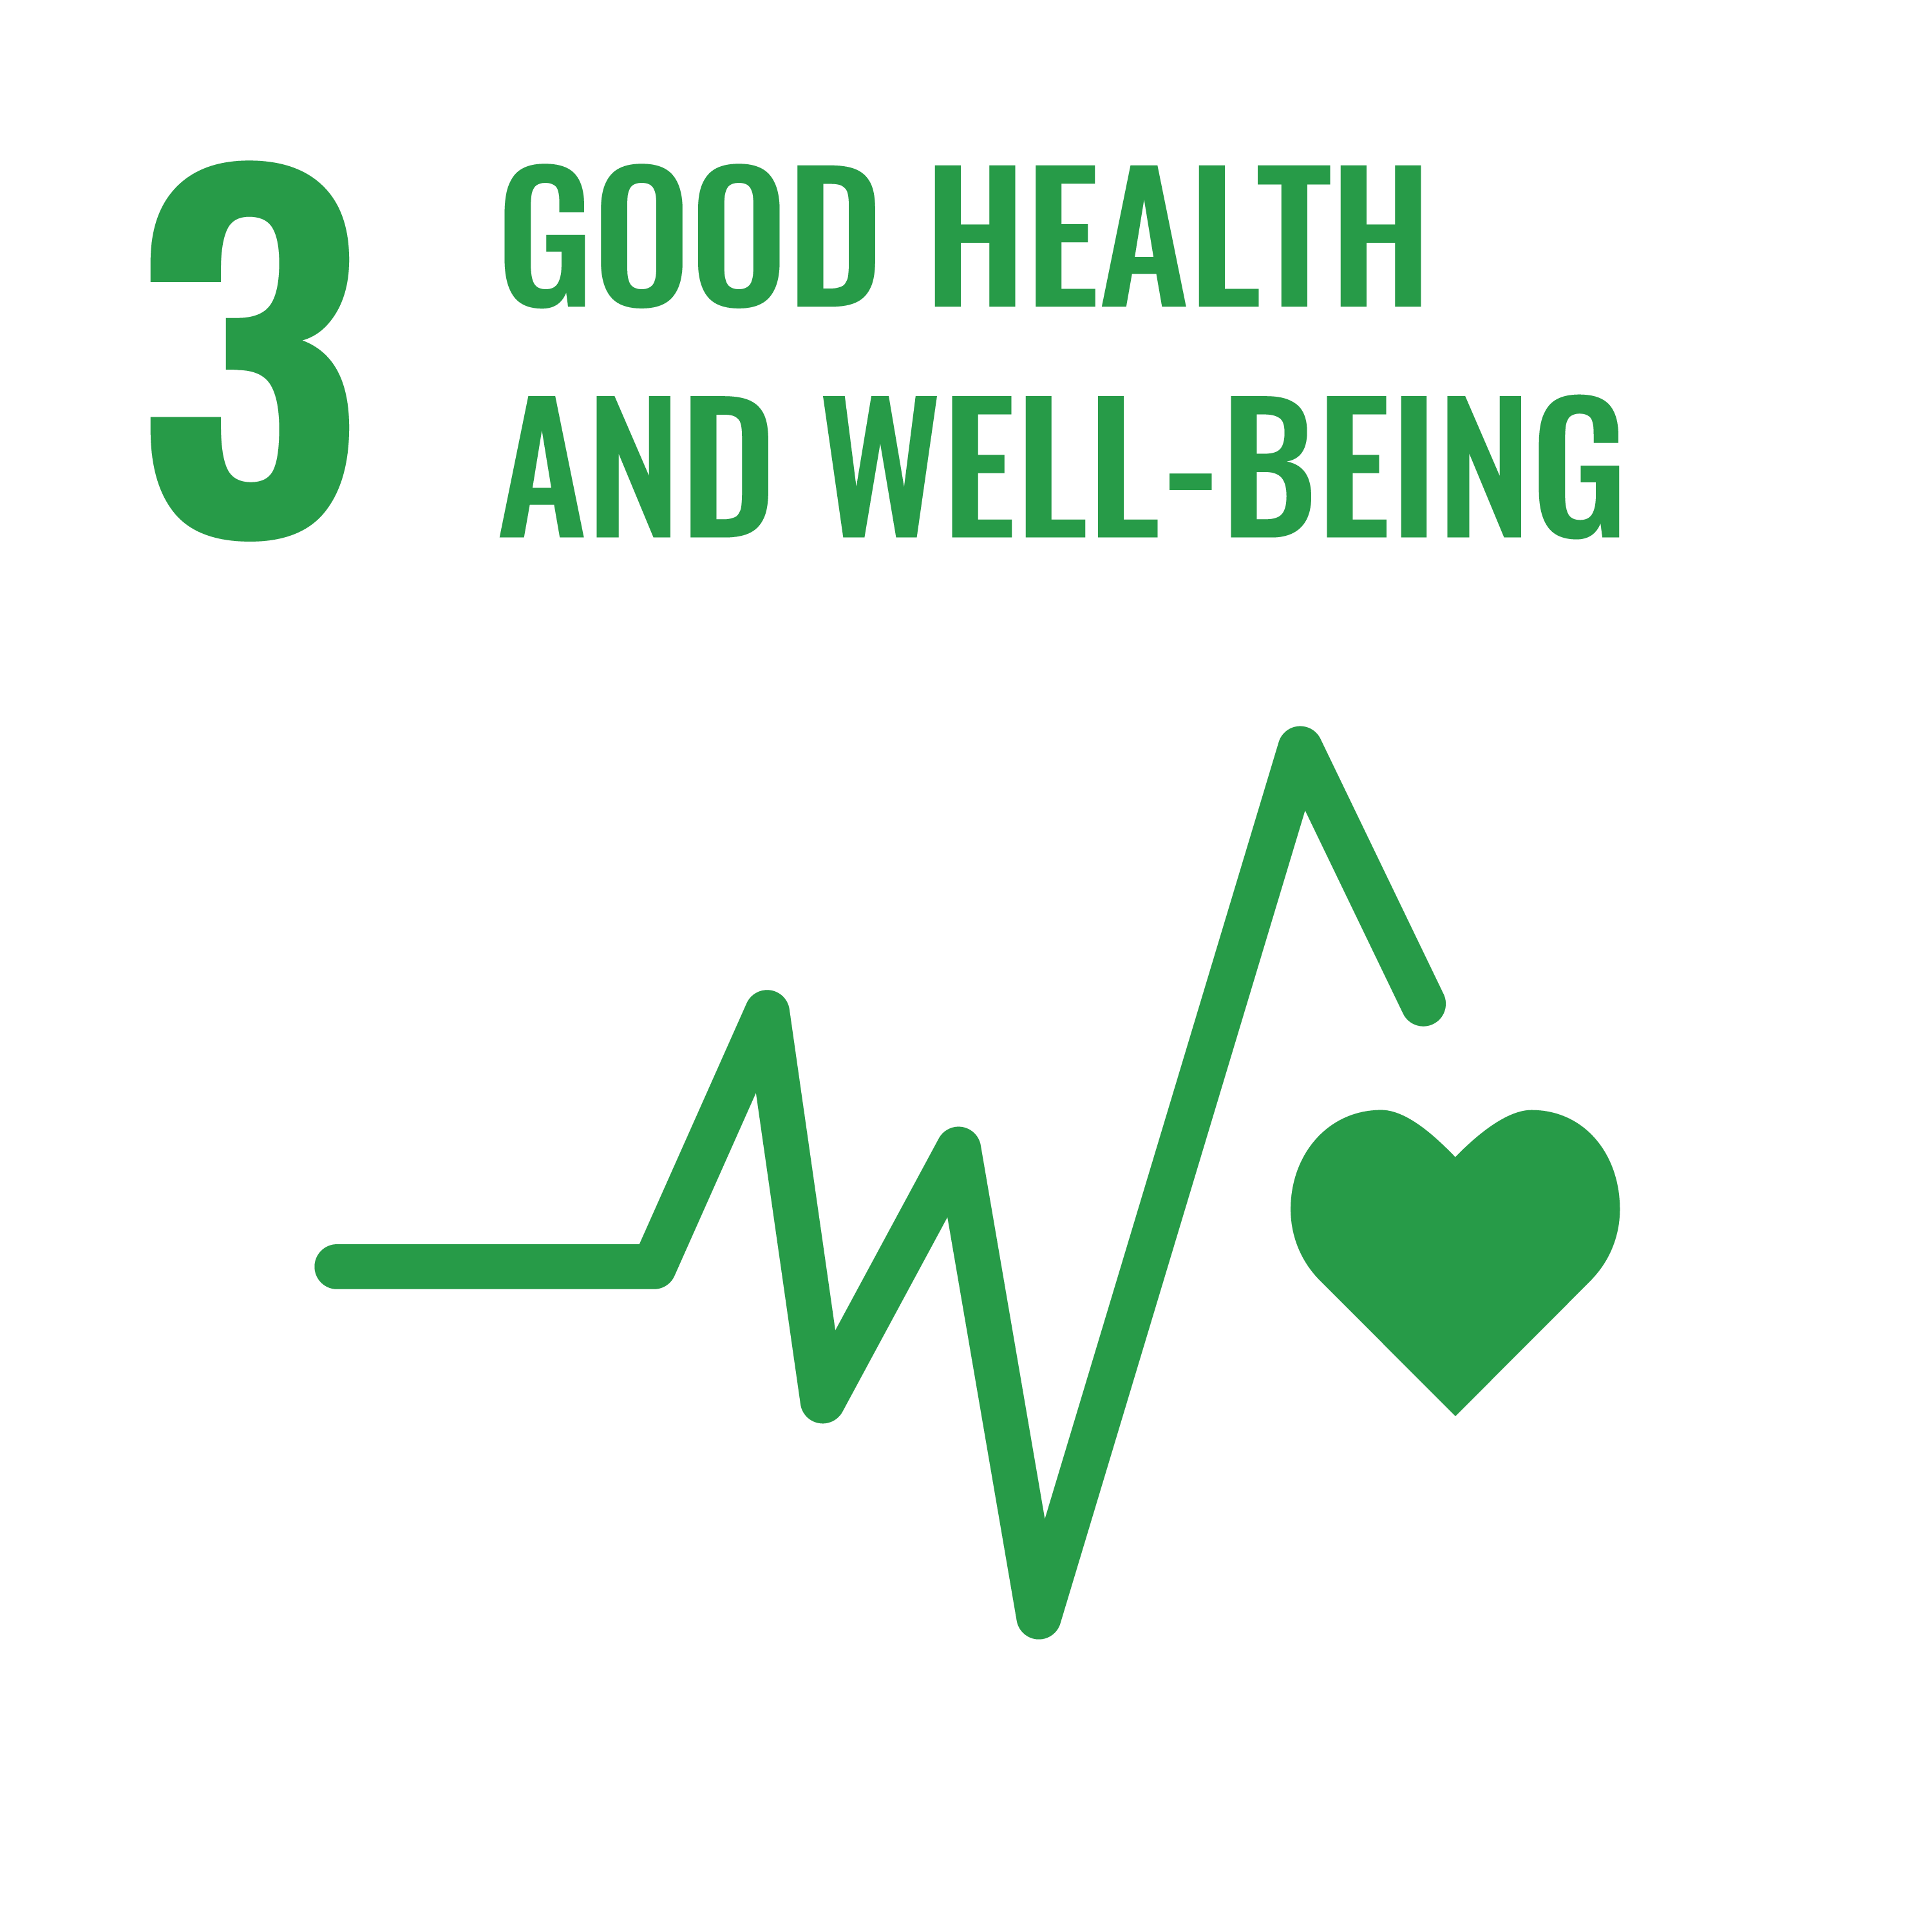
\includegraphics[scale=\SDGscale]{Sections/Figs/Common/SDG_3_GoodHealth.png}}} & \parbox[t]{\SDGright\textwidth}{\textbf{3 Good health and well-being:\ Ensure healthy lives and promote well-being for all at all ages}
\vspace{\recskip}
\begin{itemize}[leftmargin=20pt]
\setlength{\itemsep}{\recskip}
\item HECAP+ research helps to develop medical diagnostics and treatments, \eg for cancer.
\item The working culture practised every day has an impact on the mental health of ourselves and co-workers.
\item The design of experimental setups has an effect on (work) safety issues.
\item Food served and consumed at institutes and events has an impact on the health and well-being of the consumers.
\end{itemize}}\\

\parbox[t]{\SDGleft\textwidth}{\raisebox{\iconskip}{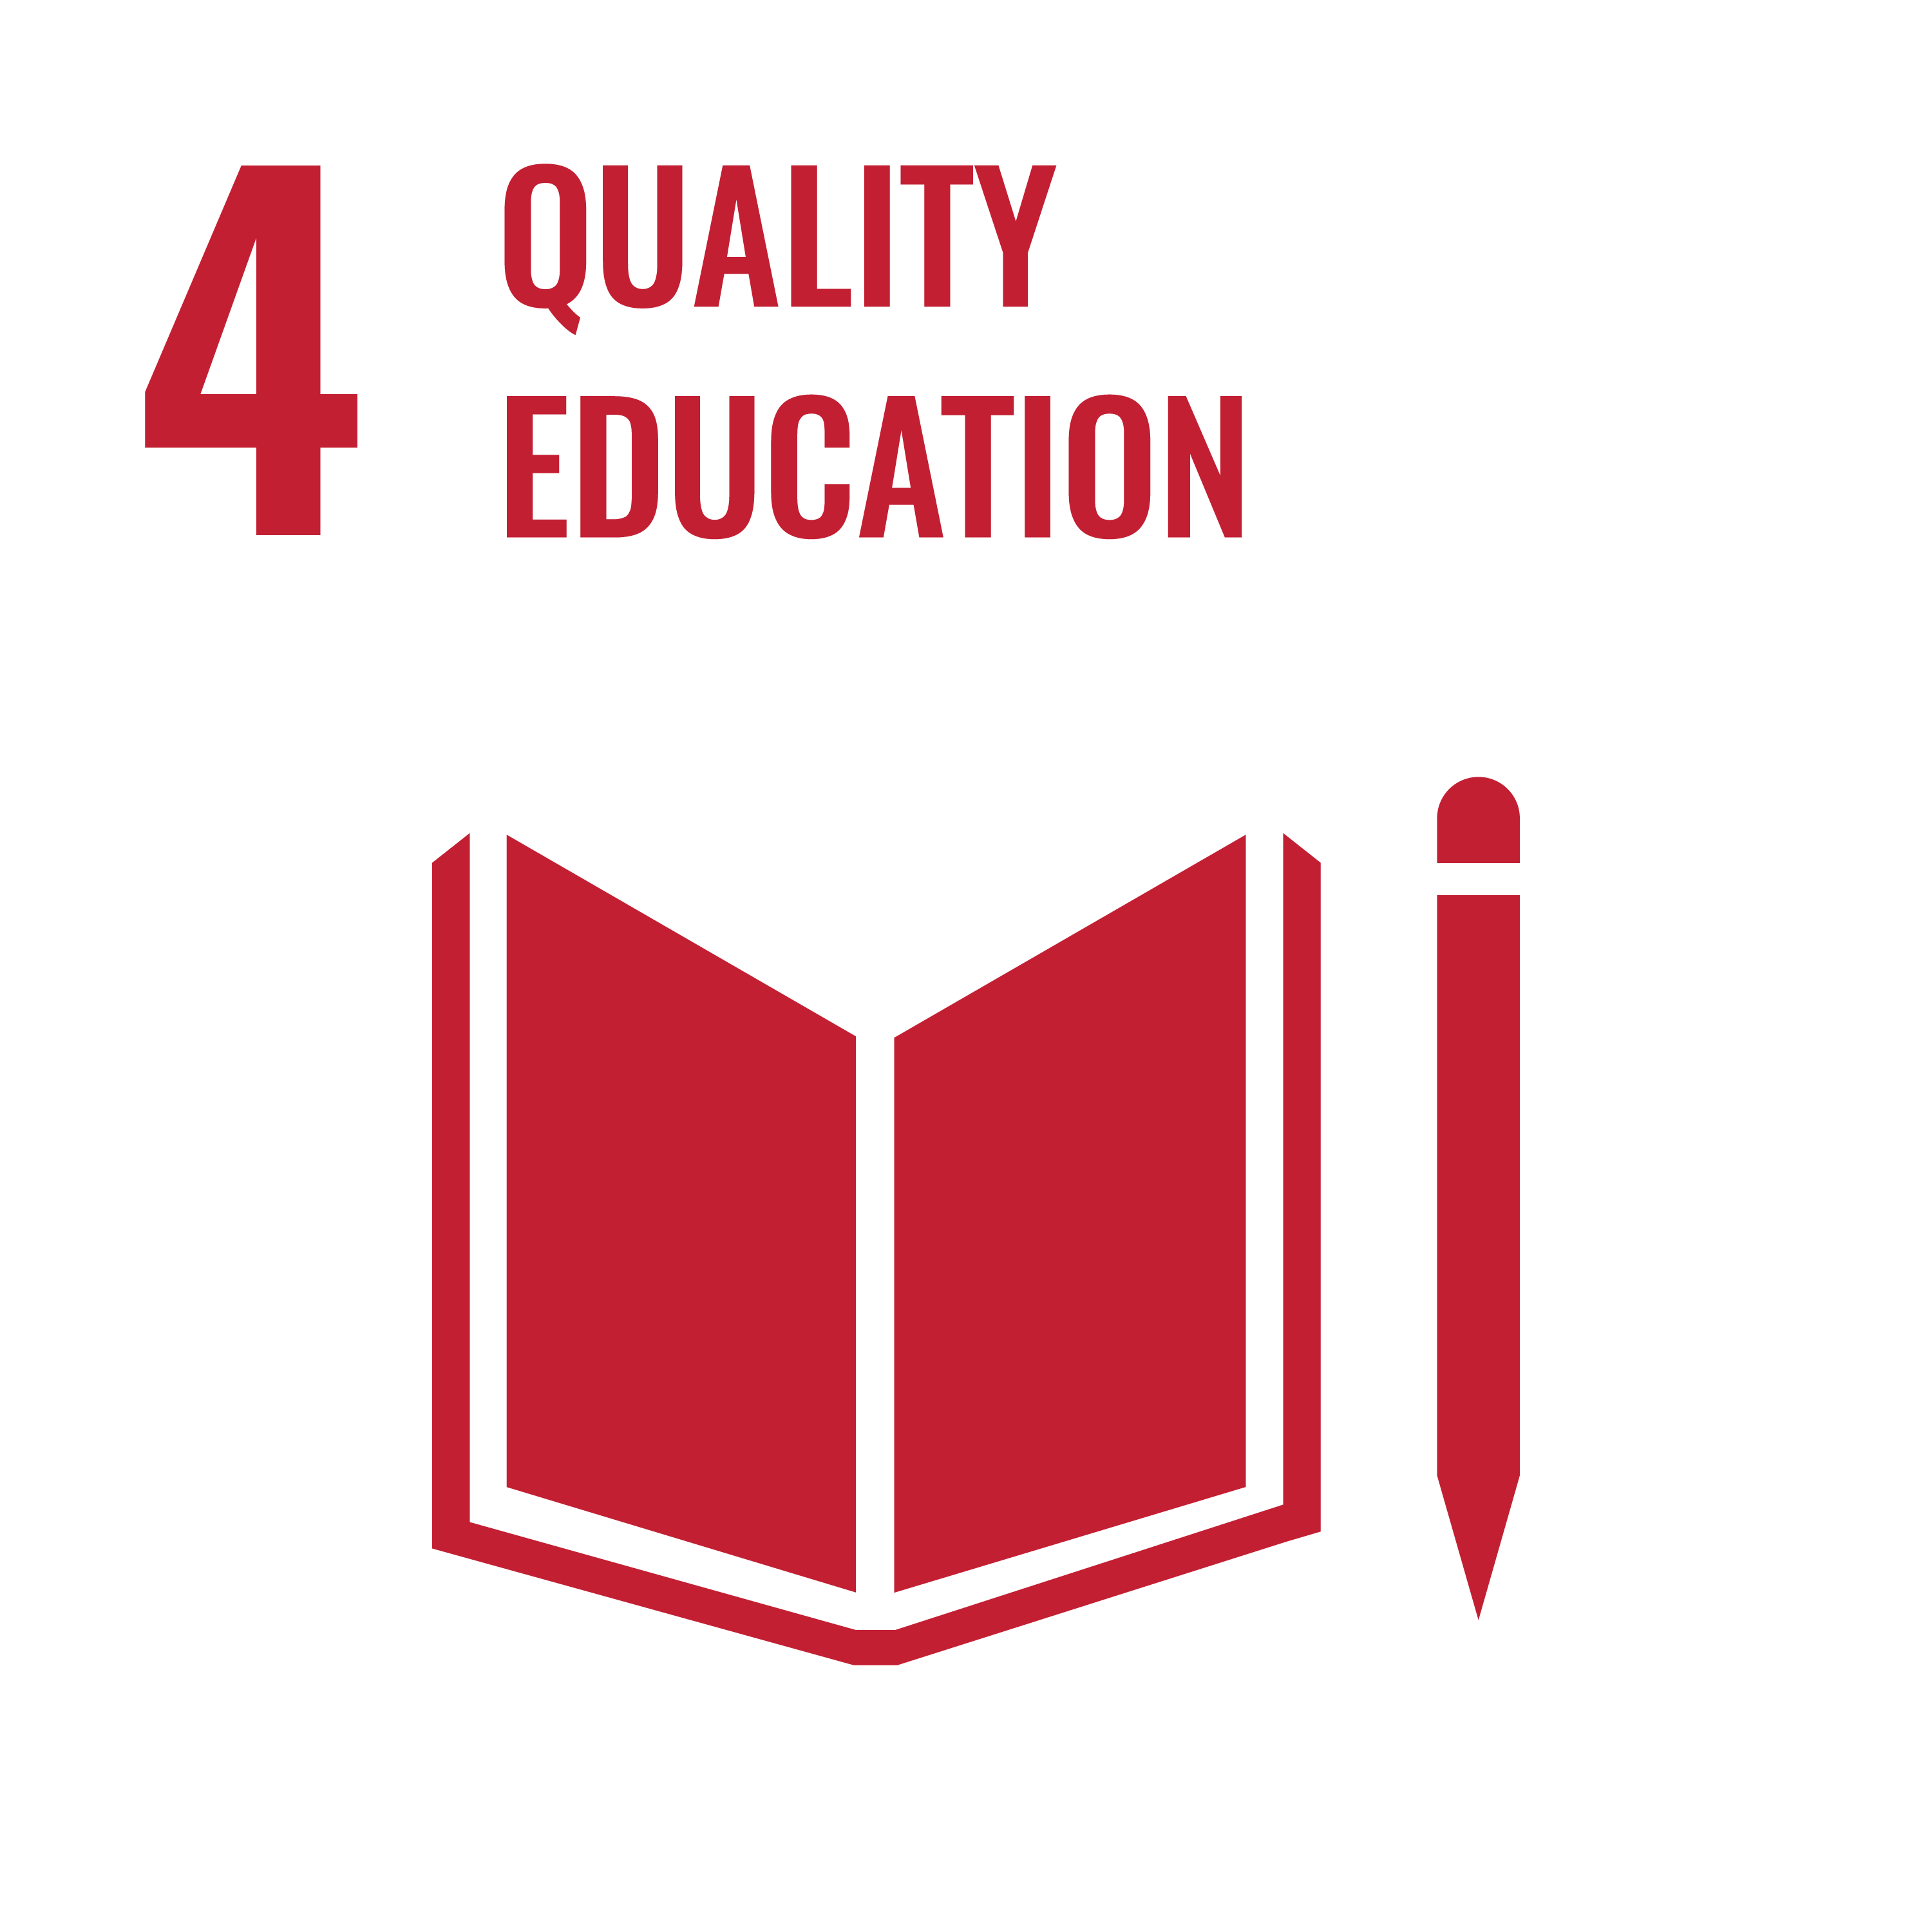
\includegraphics[scale=\SDGscale]{Sections/Figs/Common/SDG_4_QualityEducation.png}}} & \parbox[t]{\SDGright\textwidth}{\textbf{4 Quality education:\ Ensure inclusive and equitable quality education and promote lifelong learning opportunities for all}
\vspace{\recskip}
\begin{itemize}[leftmargin=20pt]
\setlength{\itemsep}{\recskip}
\item Research develops and uses scientific methods to establish a general body of knowledge that can be passed on in educational settings.
\item Researchers are often teachers for their respective field and have an effect on the teaching culture.
\item Researchers and institutes, through their conduct and integrity, have an impact on the credibility of science in society.
\item Transparent reporting on efforts towards more sustainable research has a positive impact on the credibility of scientists, and helps avoid greenwashing.
\end{itemize}}\\

\parbox[t]{\SDGleft\textwidth}{\raisebox{\iconskip}{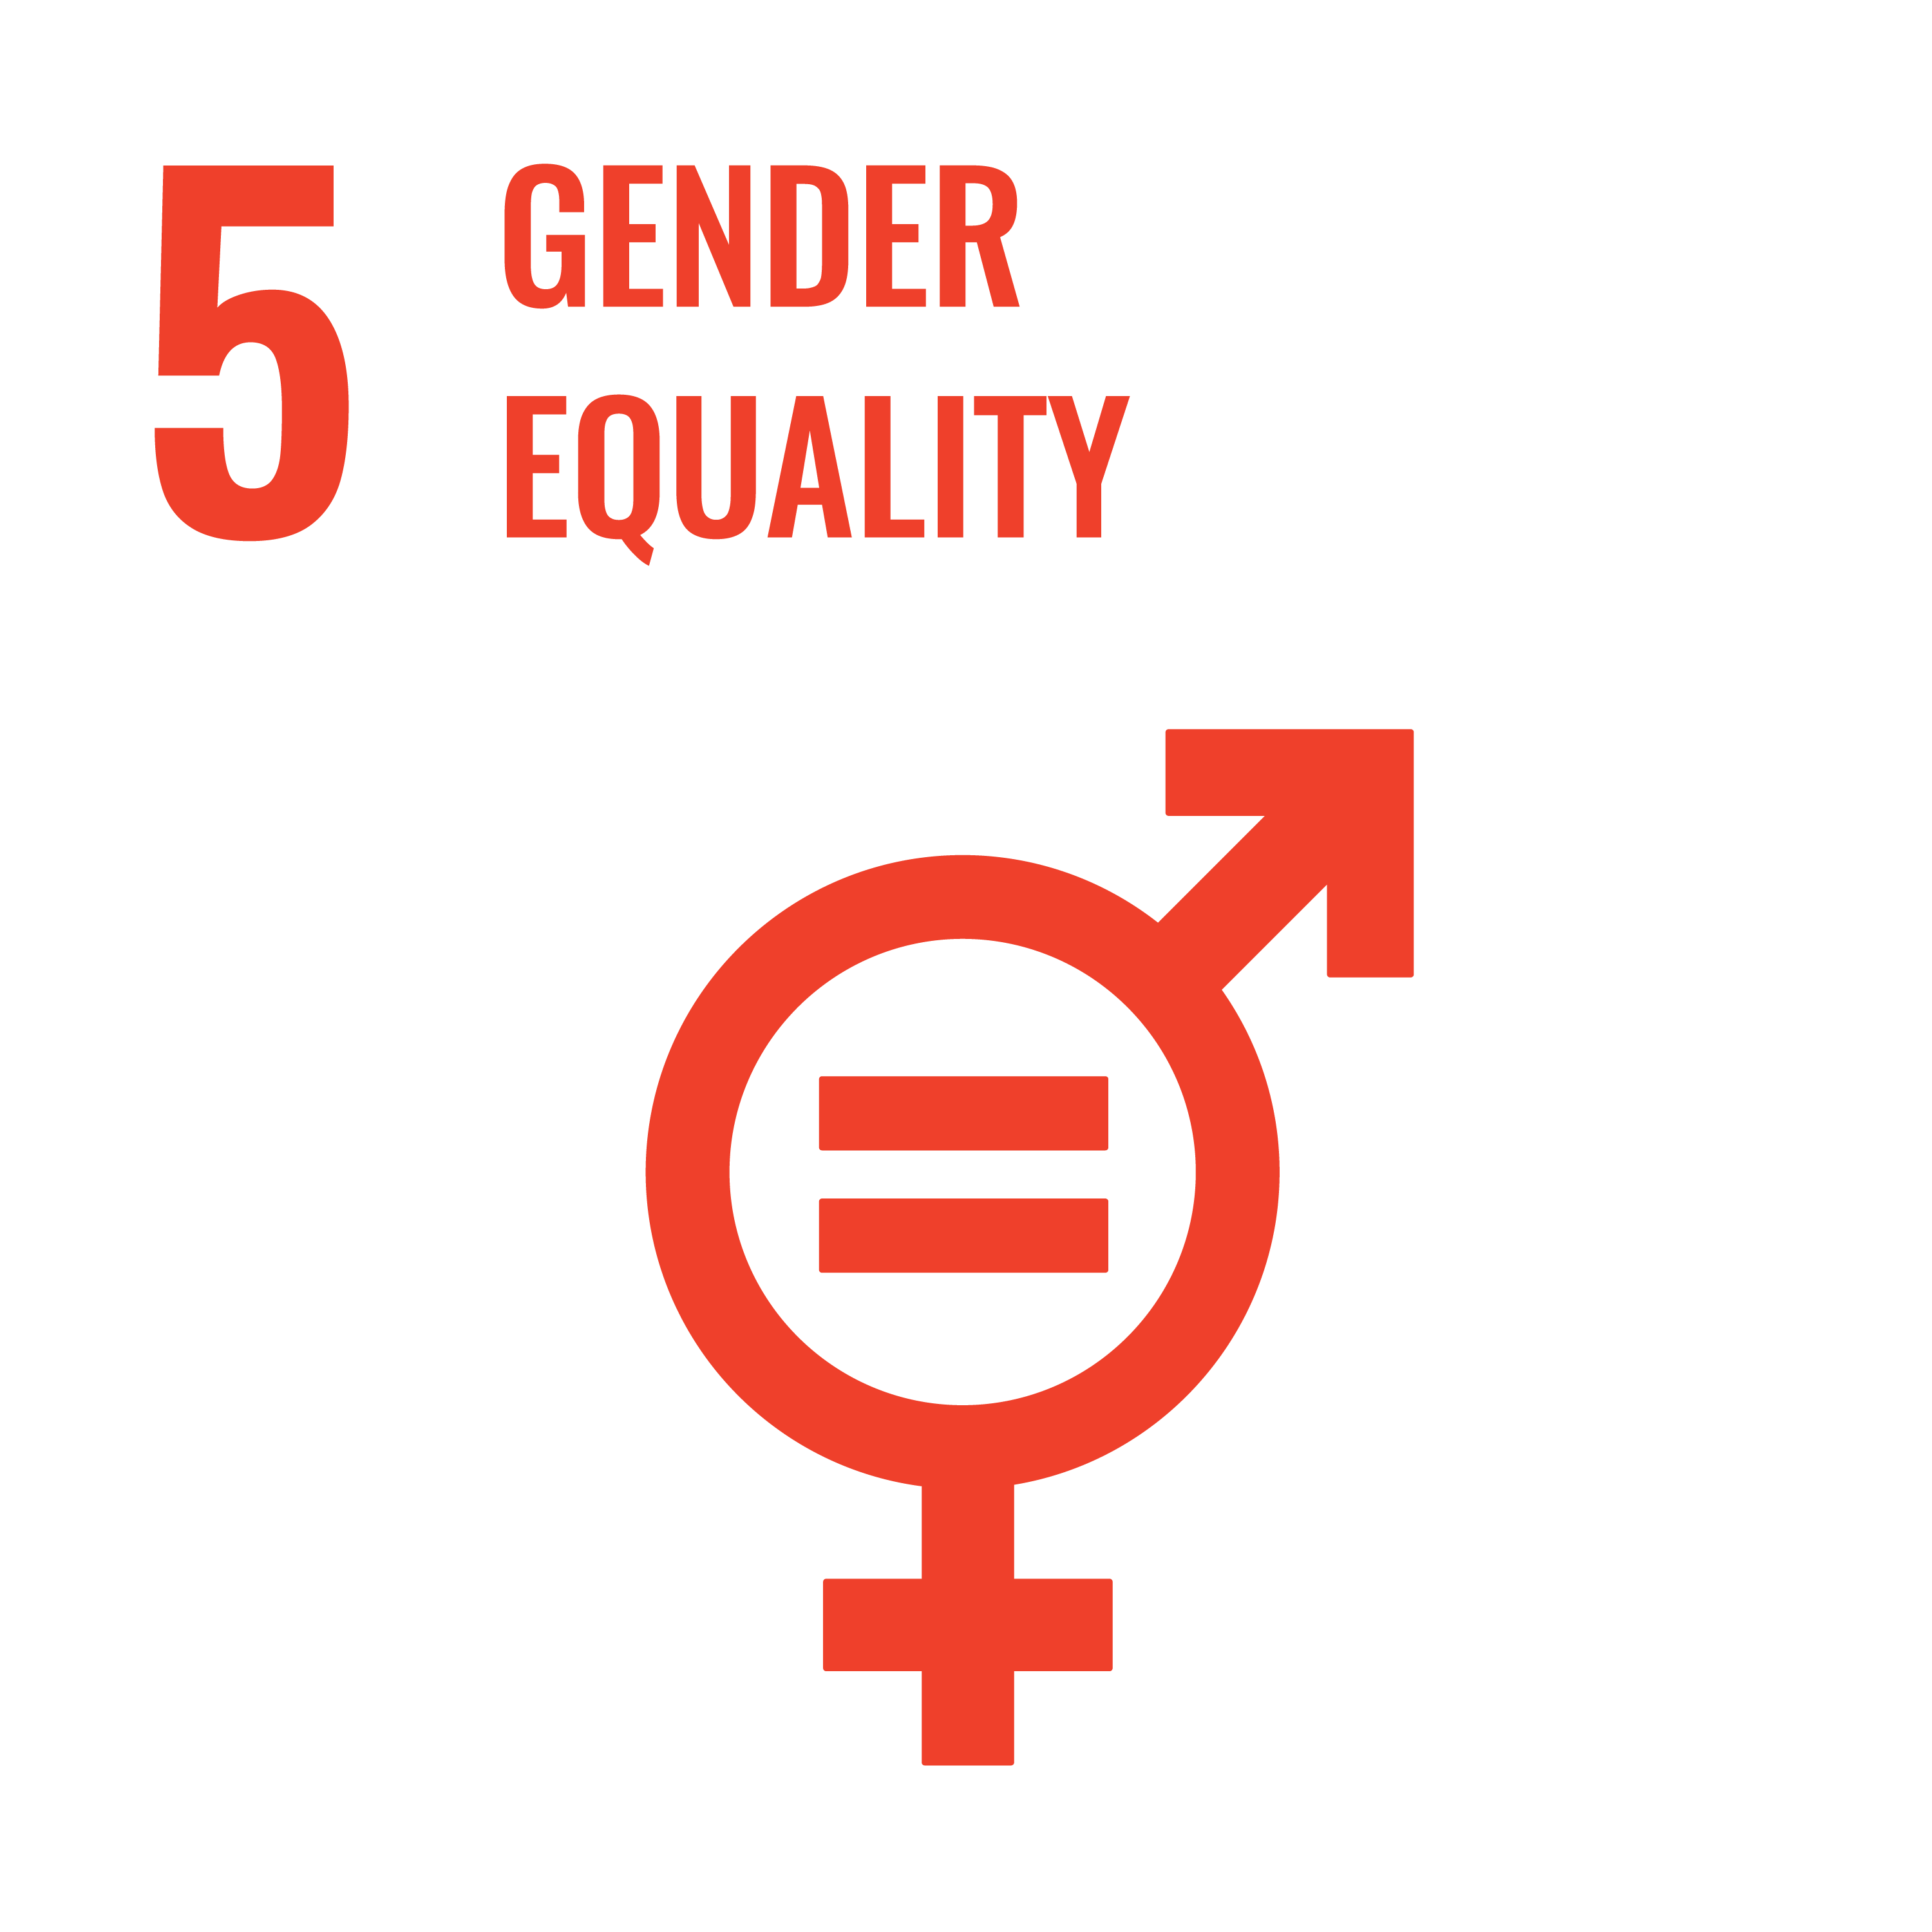
\includegraphics[scale=\SDGscale]{Sections/Figs/Common/SDG_5_GenderEquality.png}}} & \parbox[t]{\SDGright\textwidth}{\textbf{5 Gender equality:\ Achieve gender equality and empower all women and girls}
\vspace{\recskip}
\begin{itemize}[leftmargin=20pt]
\setlength{\itemsep}{\recskip}
\item As an historically male-dominated field, \ACR\ should strive to act for the visibility, acceptance and representative participation of all genders.
\end{itemize}}\\

\parbox[t]{\SDGleft\textwidth}{\raisebox{\iconskip}{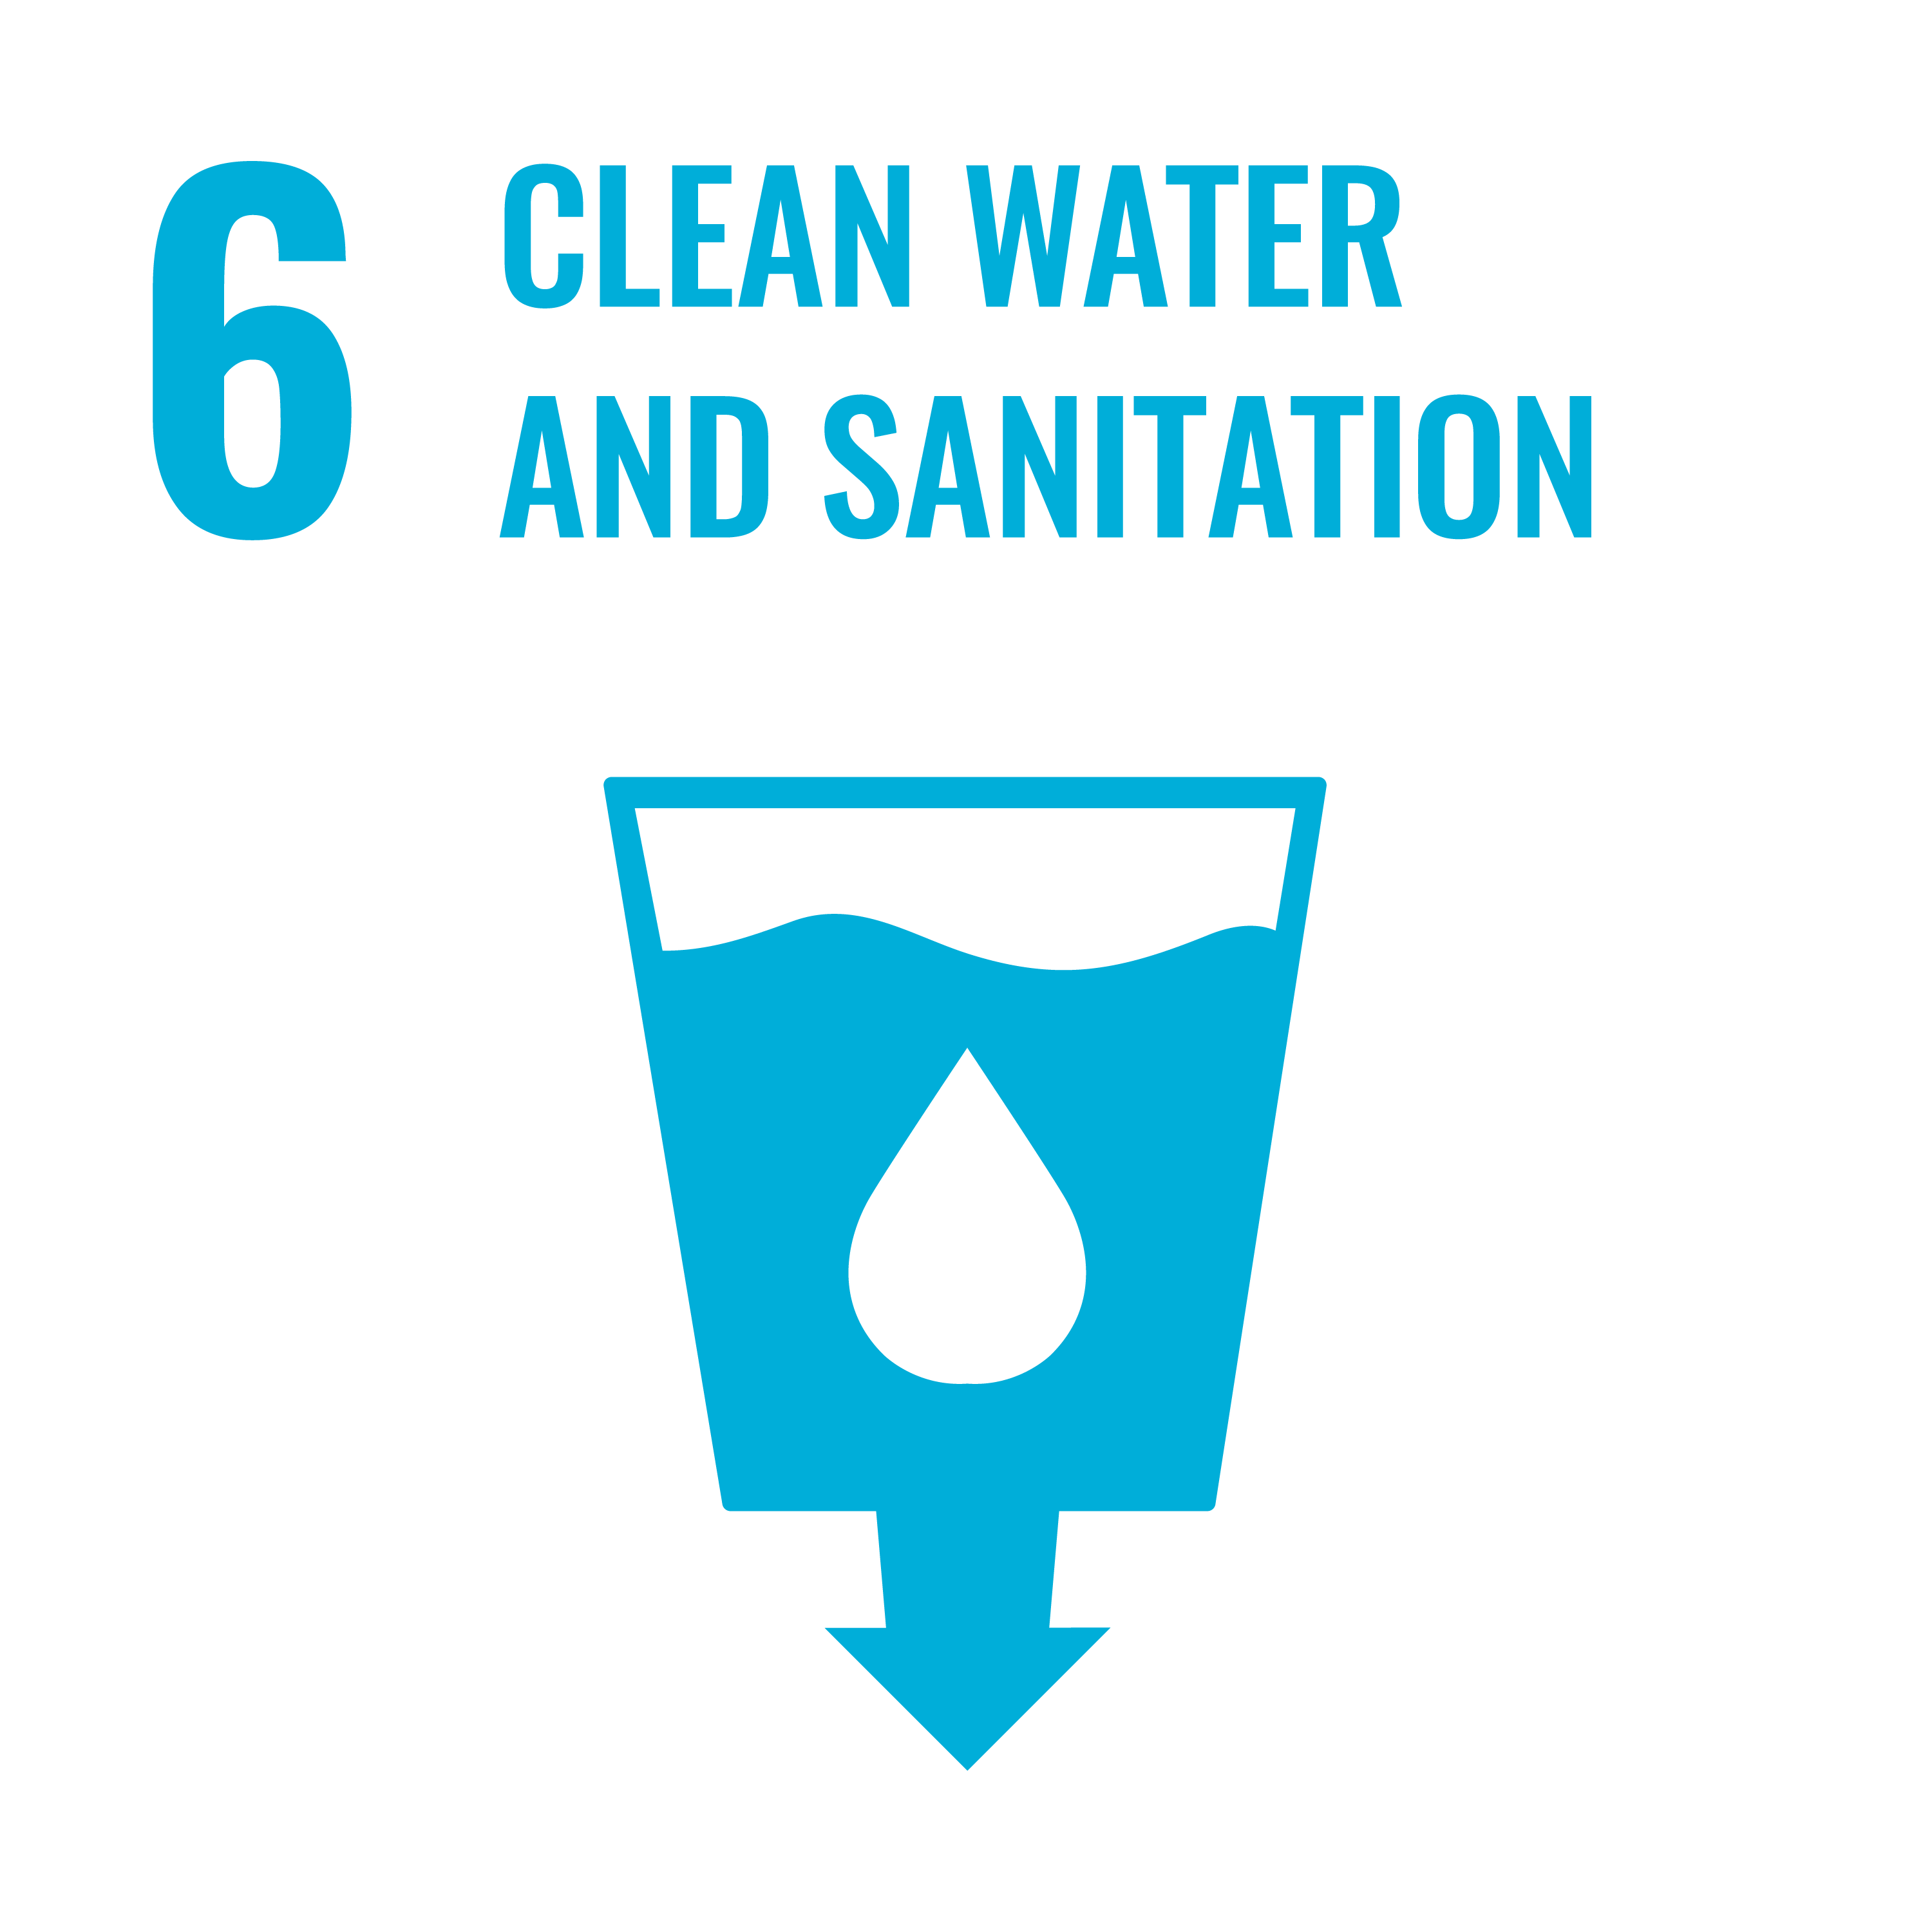
\includegraphics[scale=\SDGscale]{Sections/Figs/Common/SDG_6_CleanWater.png}}} & \parbox[t]{\SDGright\textwidth}{\textbf{6 Clean water and sanitation:\ Ensure availability and sustainable management of water and sanitation for all}
\vspace{\recskip}
\begin{itemize}[leftmargin=20pt]
\setlength{\itemsep}{\recskip}
\item Our research requires the use of water for various purposes  (heating, cooling, cleaning, sanitation, food production and preparation, etc.). Its sources are affected by our needs and behaviour.
\item \ACR\ research creates waste water. The treatment of this has an impact on the water quality in the linked aquatic ecosystems.
\item The behaviour and lifestyle choices of our community in professional and private life have an impact on the water needs in the surrounding and indirectly linked area.
\end{itemize}}\\

\parbox[t]{\SDGleft\textwidth}{\raisebox{\iconskip}{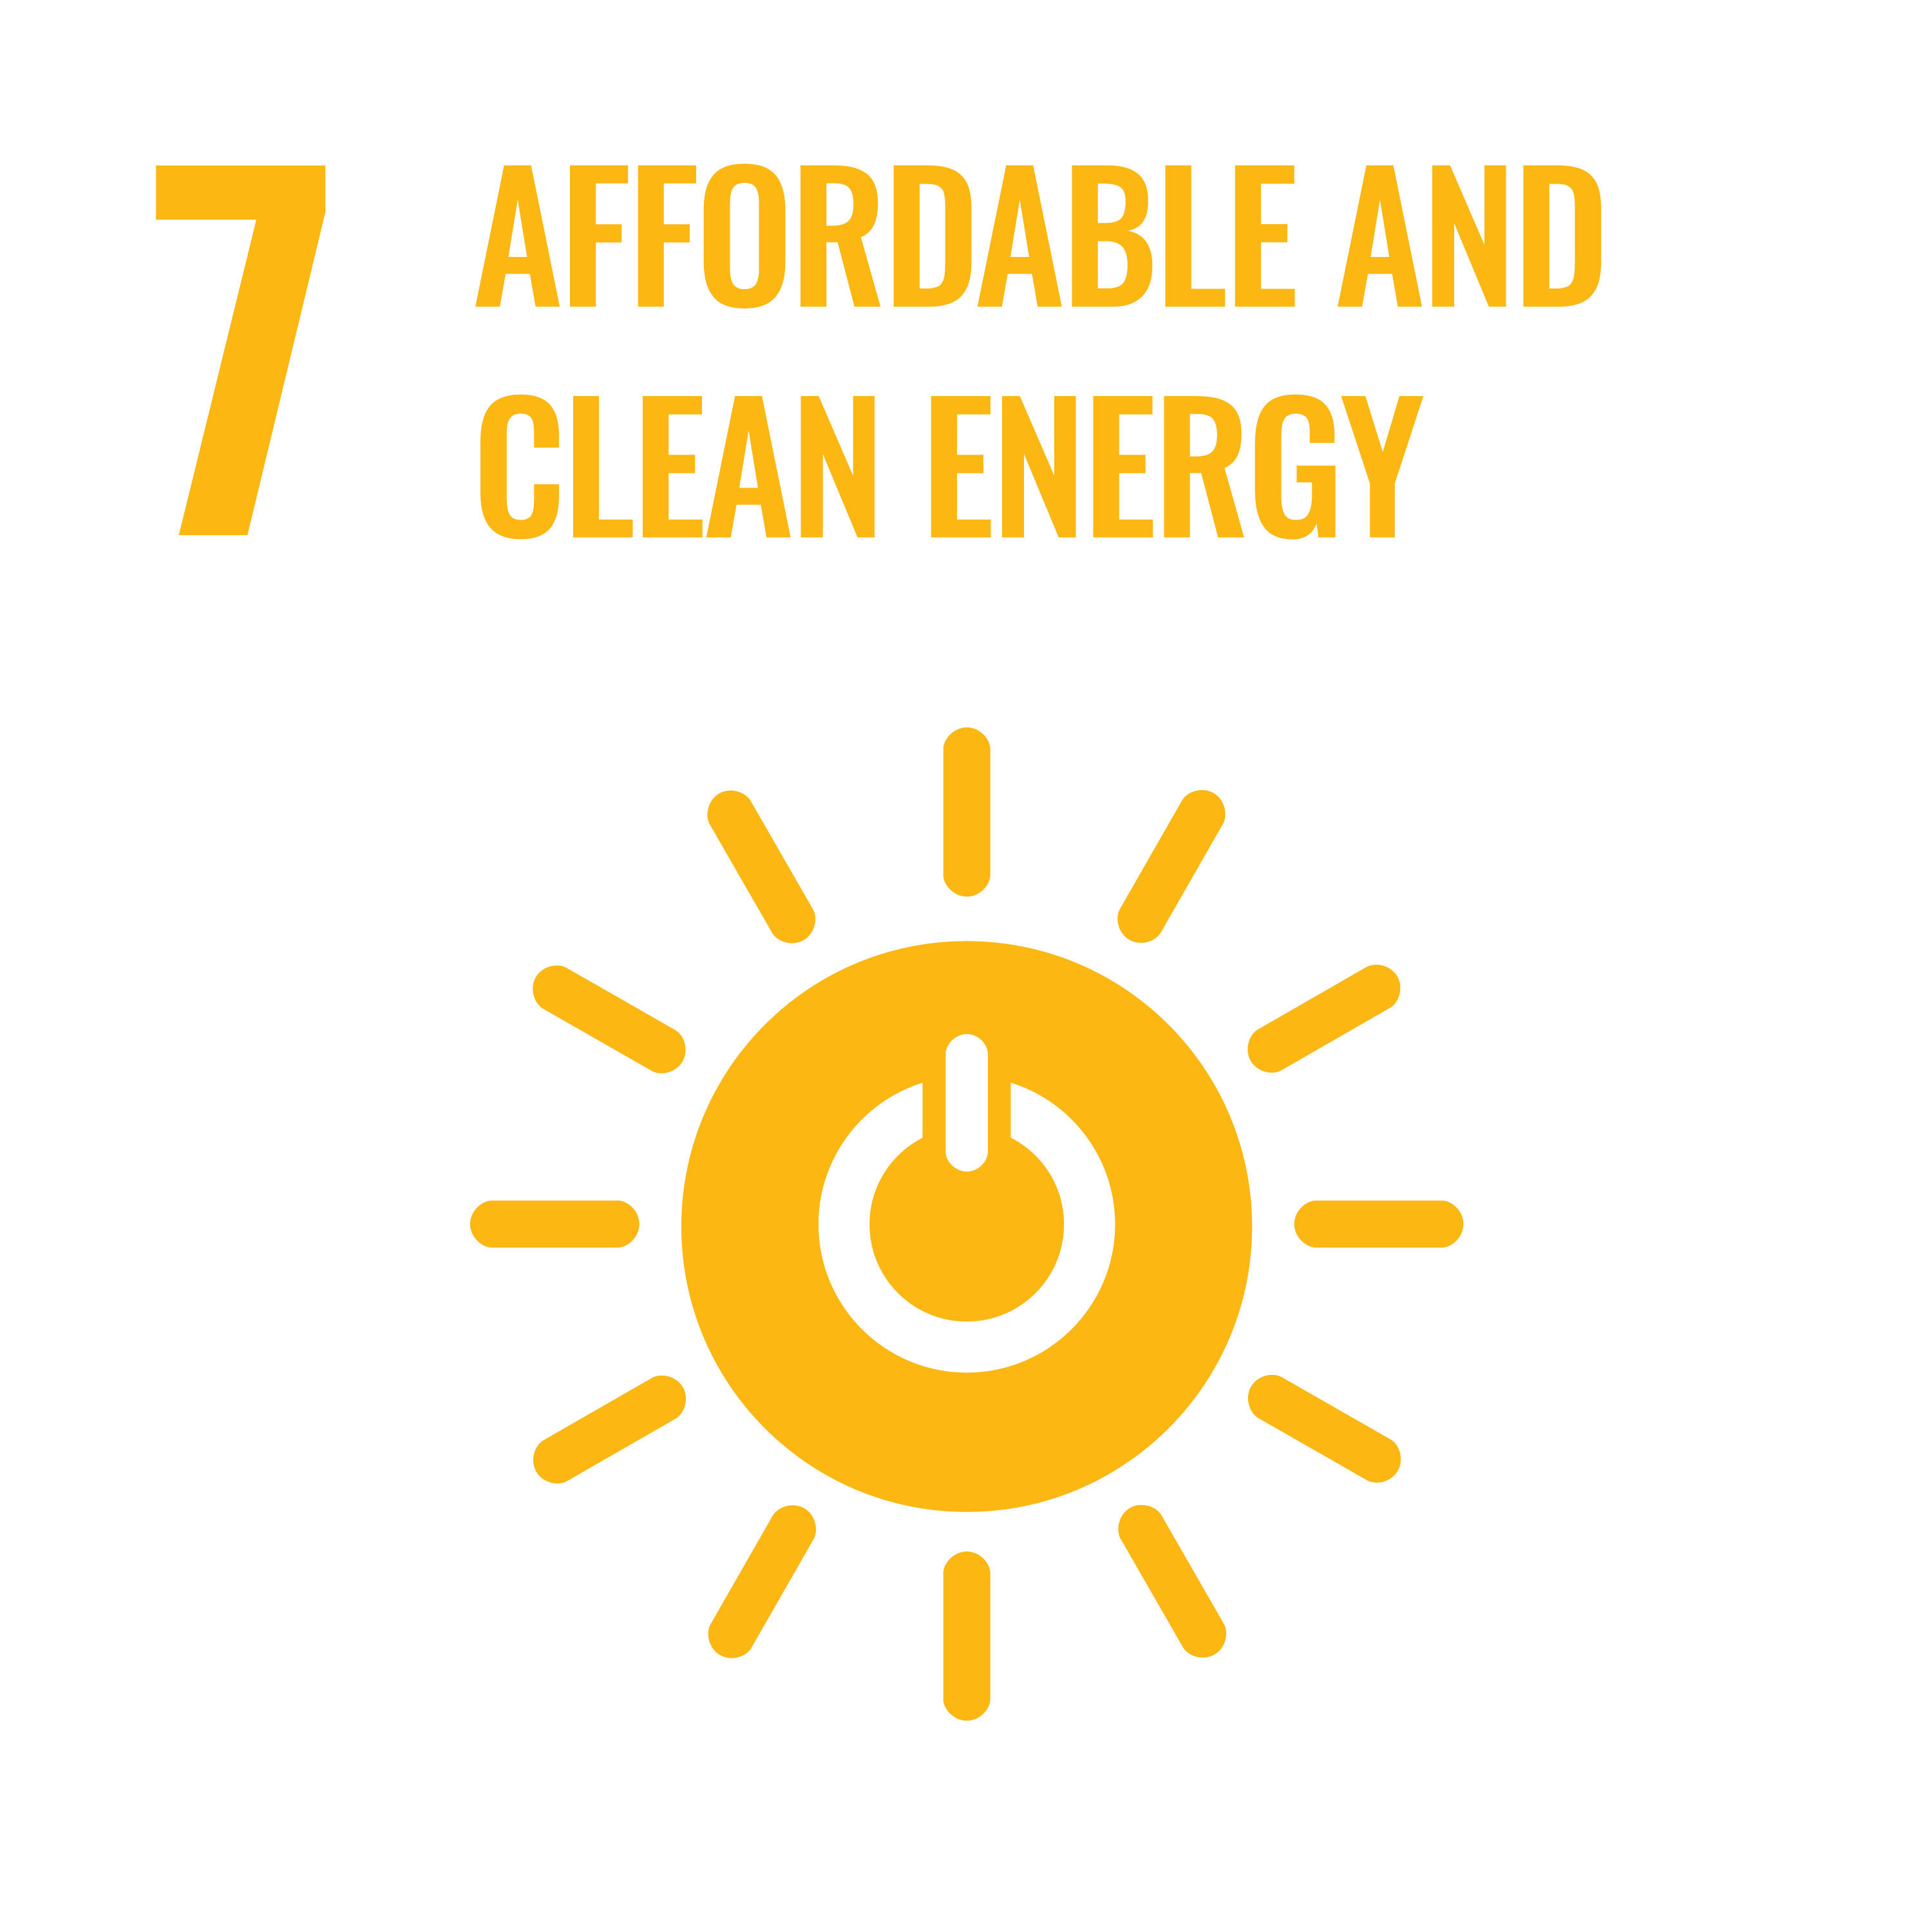
\includegraphics[scale=\SDGscale]{Sections/Figs/Common/SDG_7_CleanEnergy.png}}} & \parbox[t]{\SDGright\textwidth}{\textbf{7 Affordable and clean energy:\ Ensure access to affordable, reliable, sustainable and modern energy for all}
\vspace{\recskip}
\begin{itemize}[leftmargin=20pt]
\setlength{\itemsep}{\recskip}
\item The sources of energy planned and used for institutes, accelerators and experiments have an environmental impact on a global level.
\item The high consumption and the resulting financial impact of research facilities have an impact on the energy market.
\end{itemize}}\\

\parbox[t]{\SDGleft\textwidth}{\raisebox{\iconskip}{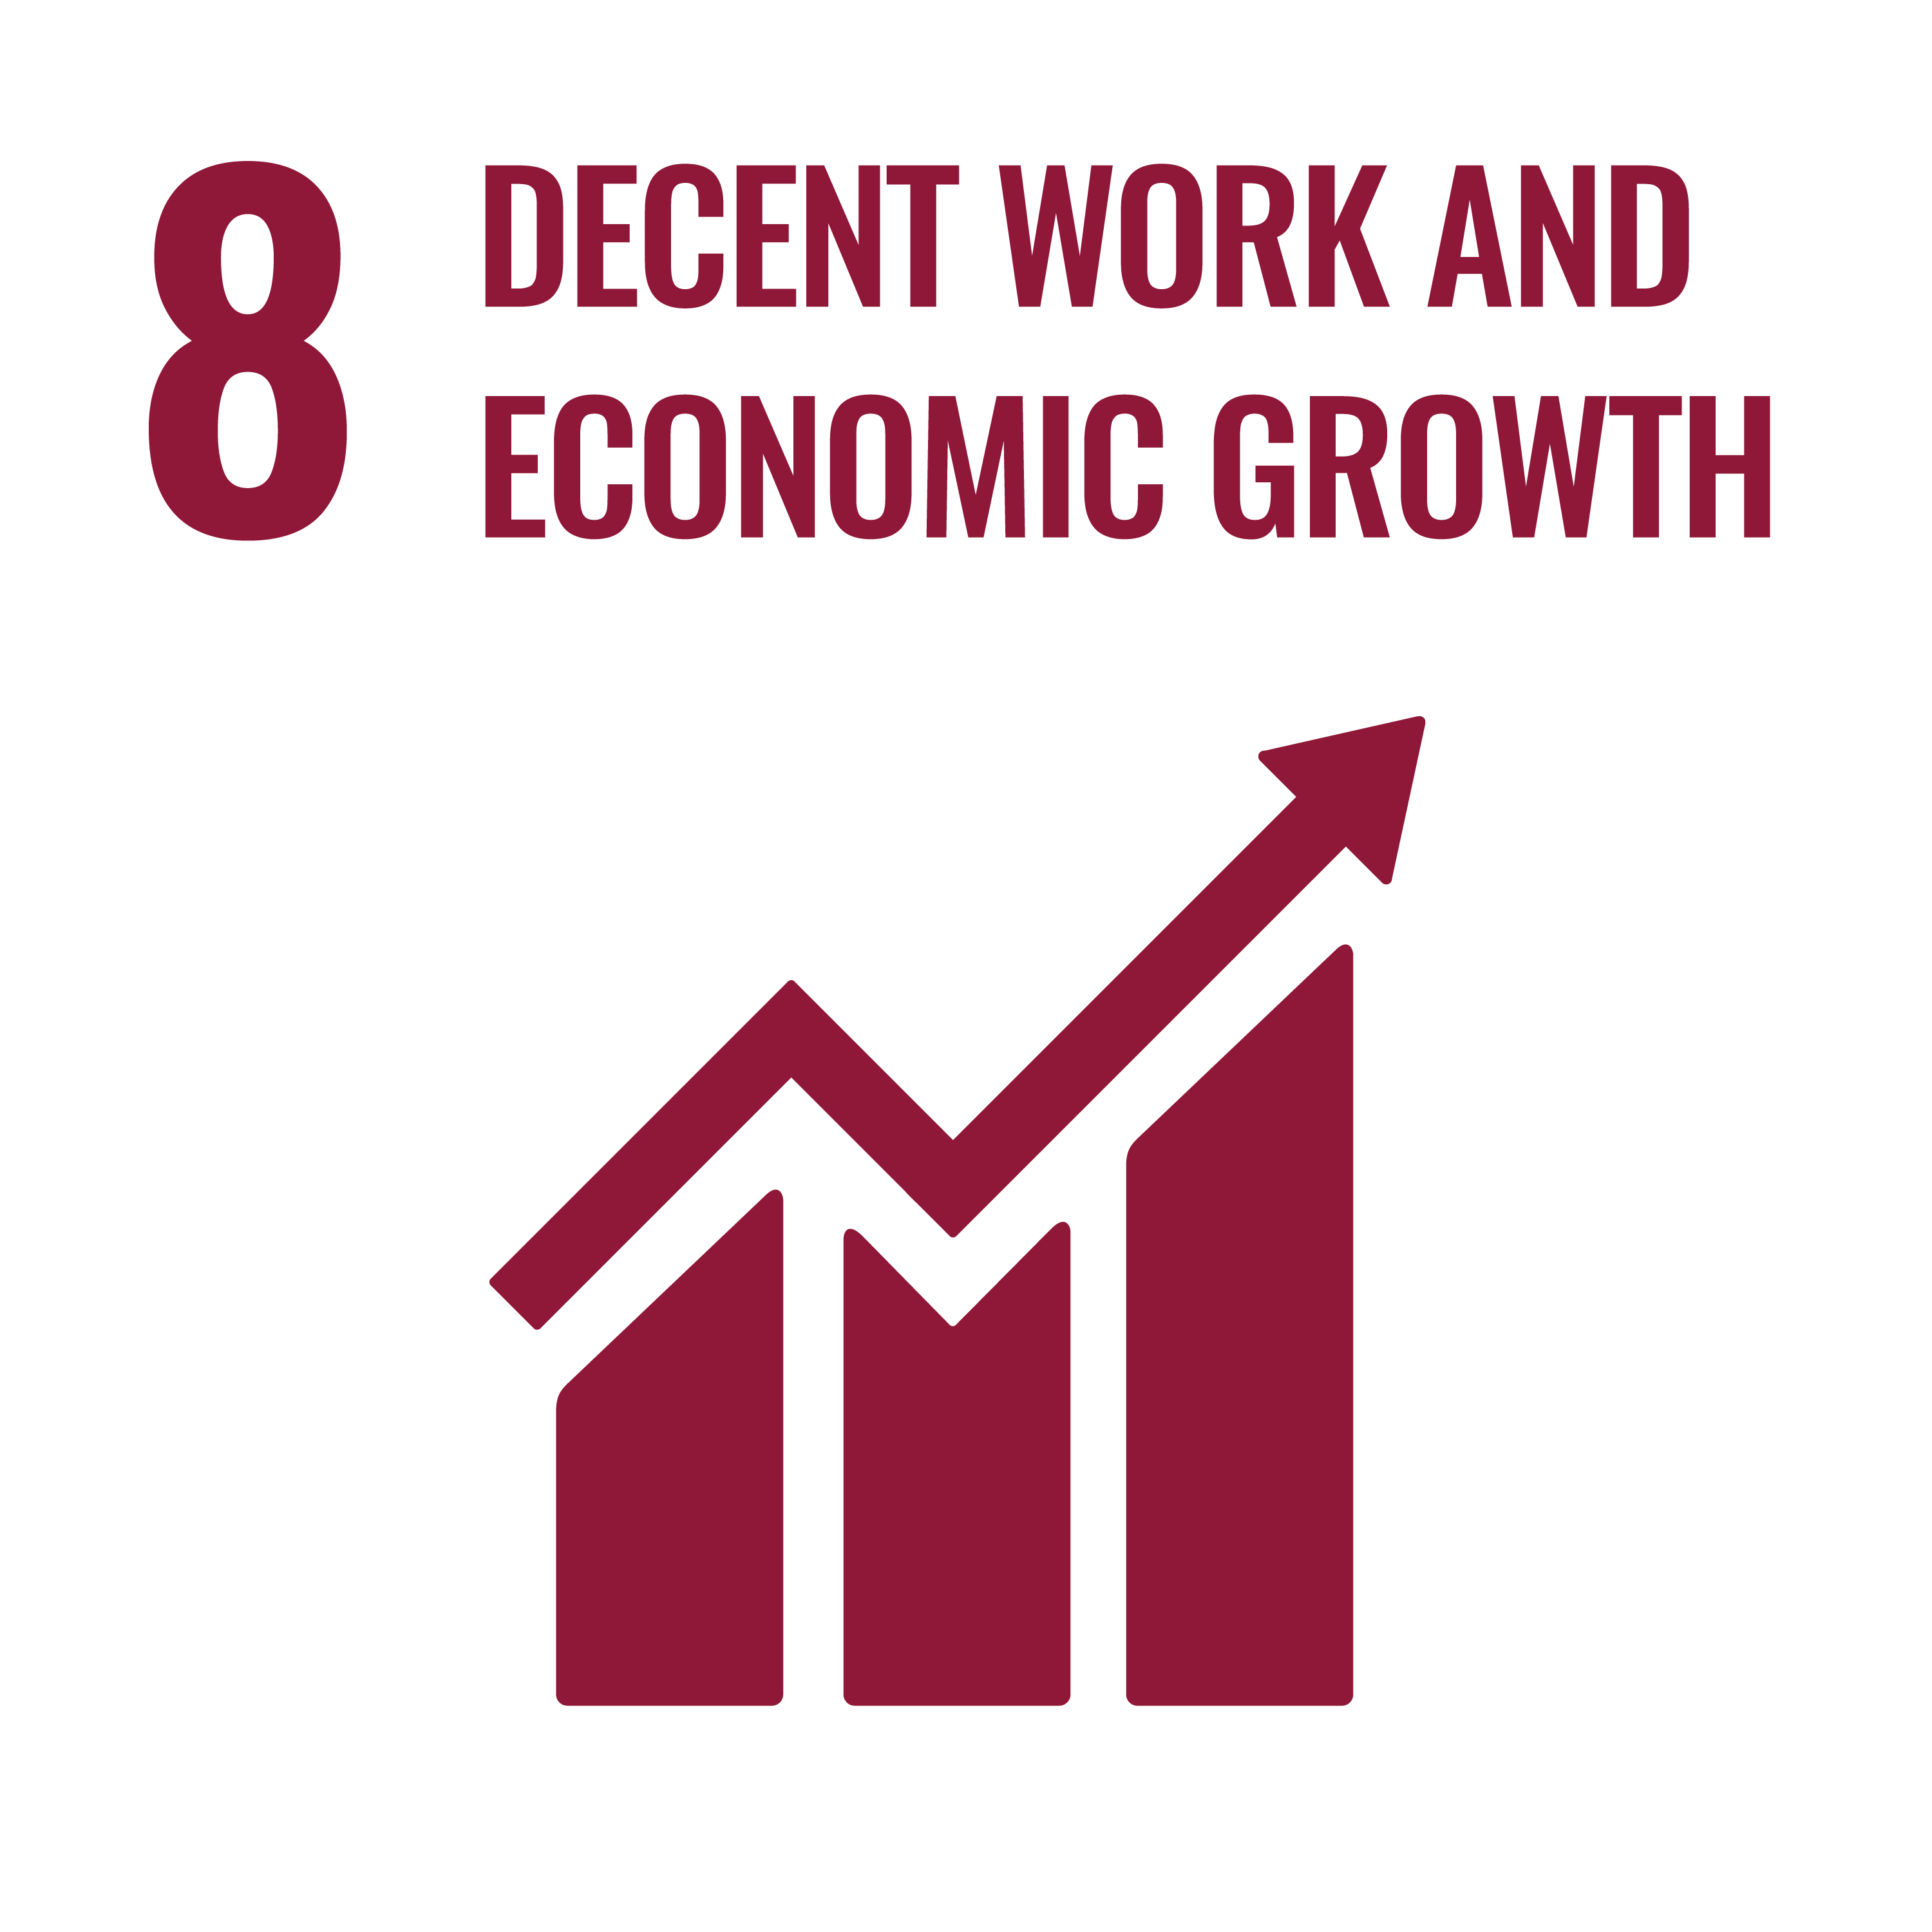
\includegraphics[scale=\SDGscale]{Sections/Figs/Common/SDG_8_EconomicGrowth.png}}} & \parbox[t]{\SDGright\textwidth}{\textbf{8 Decent work and economic growth:\ Promote sustained, inclusive and sustainable economic growth, full and productive employment and decent work for all}
\vspace{\recskip}
\begin{itemize}[leftmargin=20pt]
\setlength{\itemsep}{\recskip}
\item The terms of employment contracts and working culture in \ACR\ research influence employees' living conditions.
\end{itemize}}\\

\parbox[t]{\SDGleft\textwidth}{\raisebox{\iconskip}{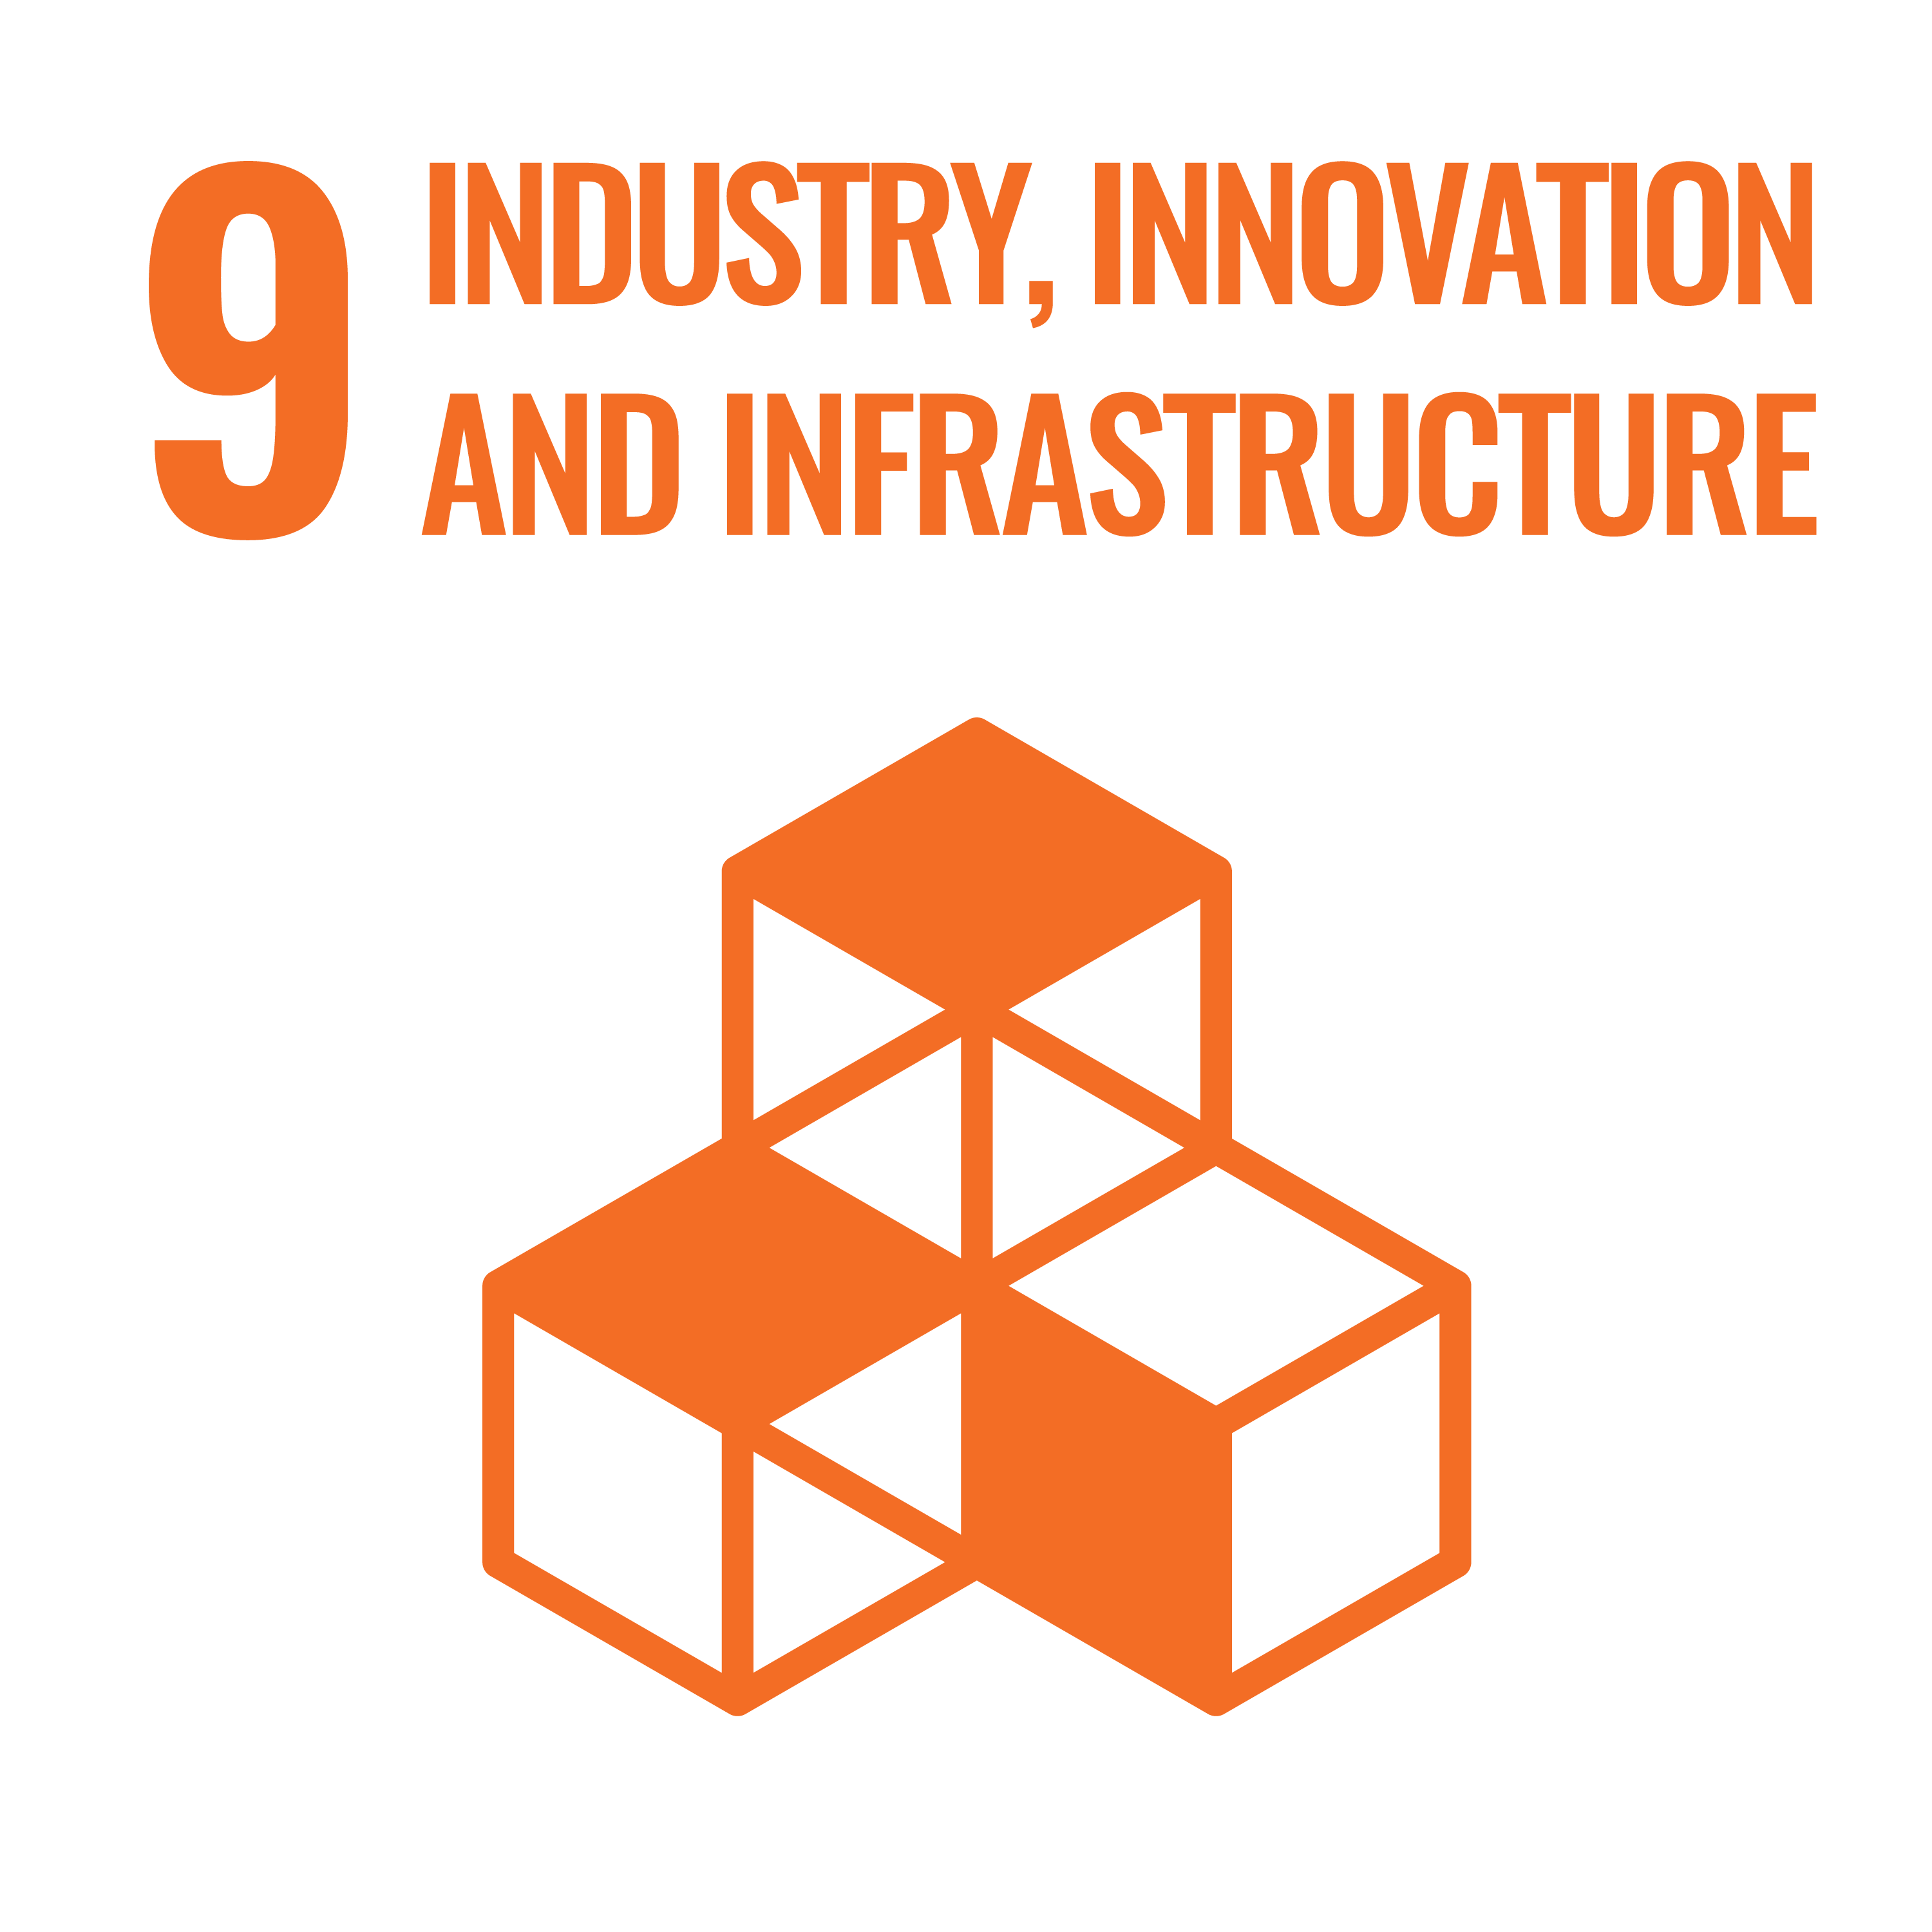
\includegraphics[scale=\SDGscale]{Sections/Figs/Common/SDG_9_IndustryInnovation.png}}} & \parbox[t]{\SDGright\textwidth}{\textbf{9 Industry, innovation and infrastructure:\ Build resilient infrastructure, promote inclusive and sustainable industrialization and foster innovation}
\vspace{\recskip}
\begin{itemize}[leftmargin=20pt]
\setlength{\itemsep}{\recskip}
\item Innovation is at the core of \ACR\ research.
\item Institutes influence the local infrastructures on which they rely and construct infrastructure for research.
\item Industry and \ACR\ research are linked as knowledge and products are transferred. This transfer can be shaped actively.
\end{itemize}}\\

\parbox[t]{\SDGleft\textwidth}{\raisebox{\iconskip}{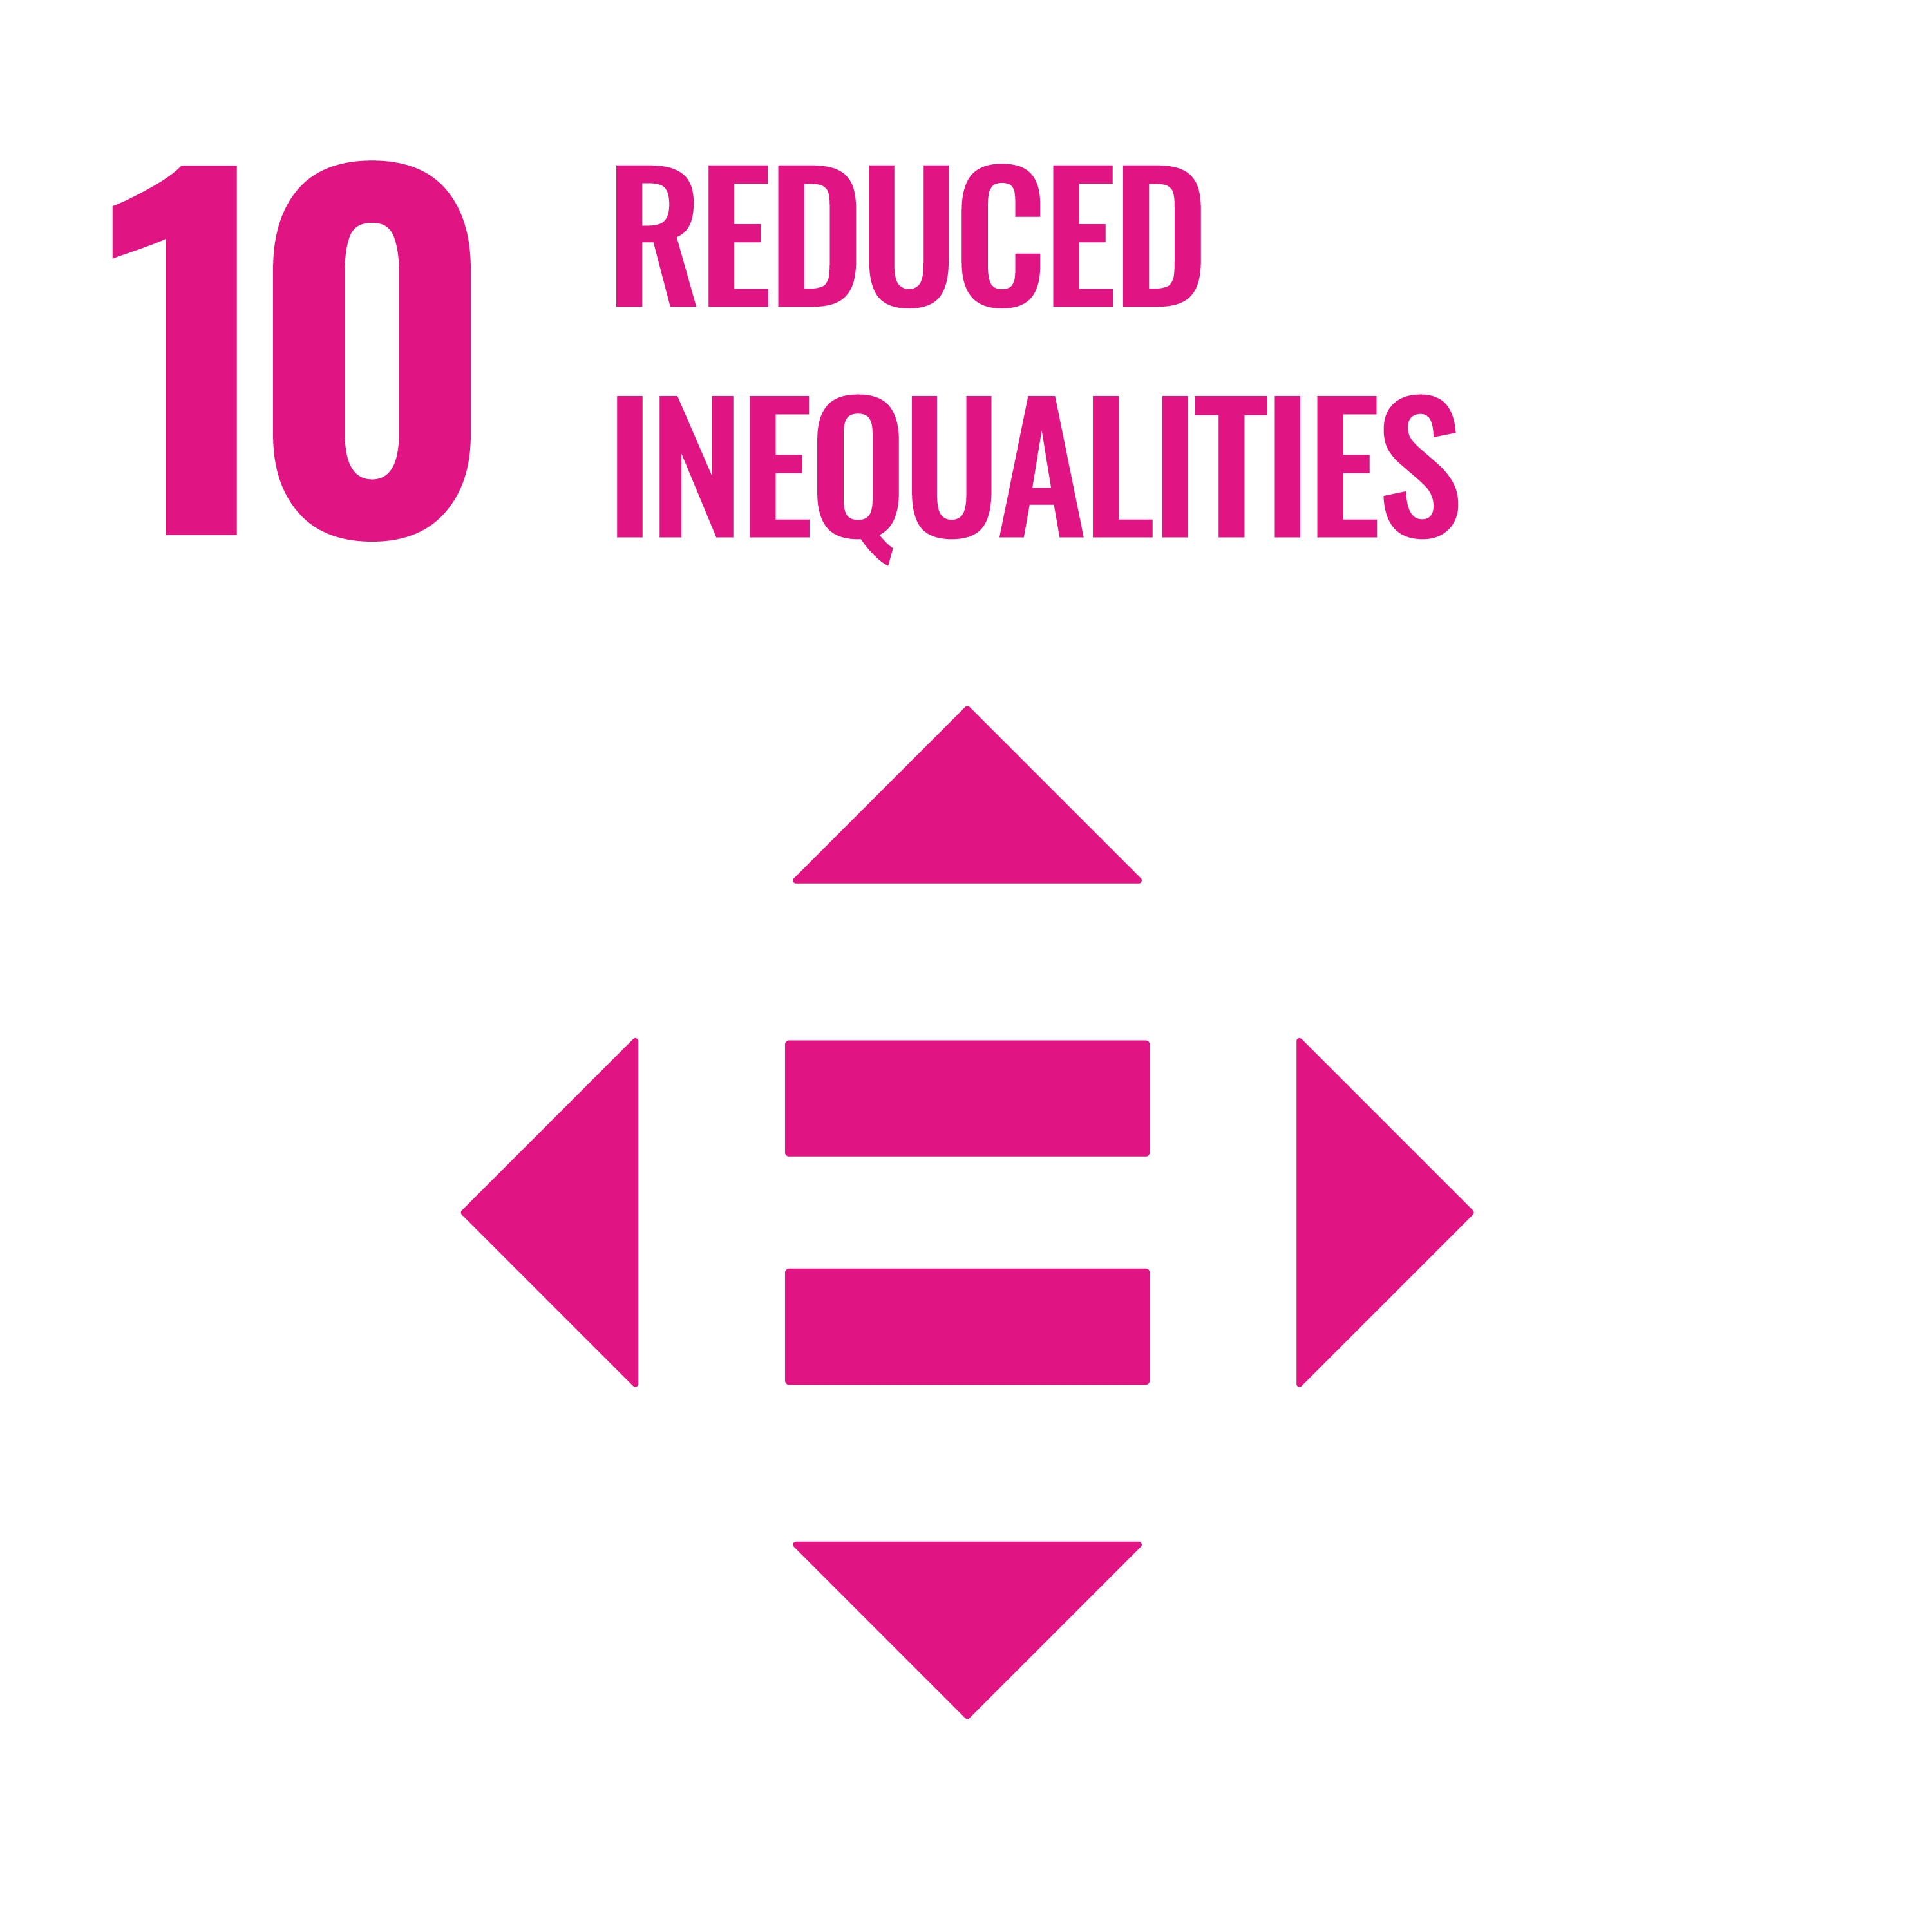
\includegraphics[scale=\SDGscale]{Sections/Figs/Common/SDG_10_ReducedInequalities.png}}} & \parbox[t]{\SDGright\textwidth}{\textbf{10 Reduced inequalities:\ Reduce inequality within and among countries}
\vspace{\recskip}
\begin{itemize}[leftmargin=20pt]
\setlength{\itemsep}{\recskip}
\item Research facilities that span multiple nations have the ability to impact the inequalities between the involved countries. They can also set examples for countries which are not (yet) involved.
\end{itemize}}\\

\parbox[t]{\SDGleft\textwidth}{\raisebox{\iconskip}{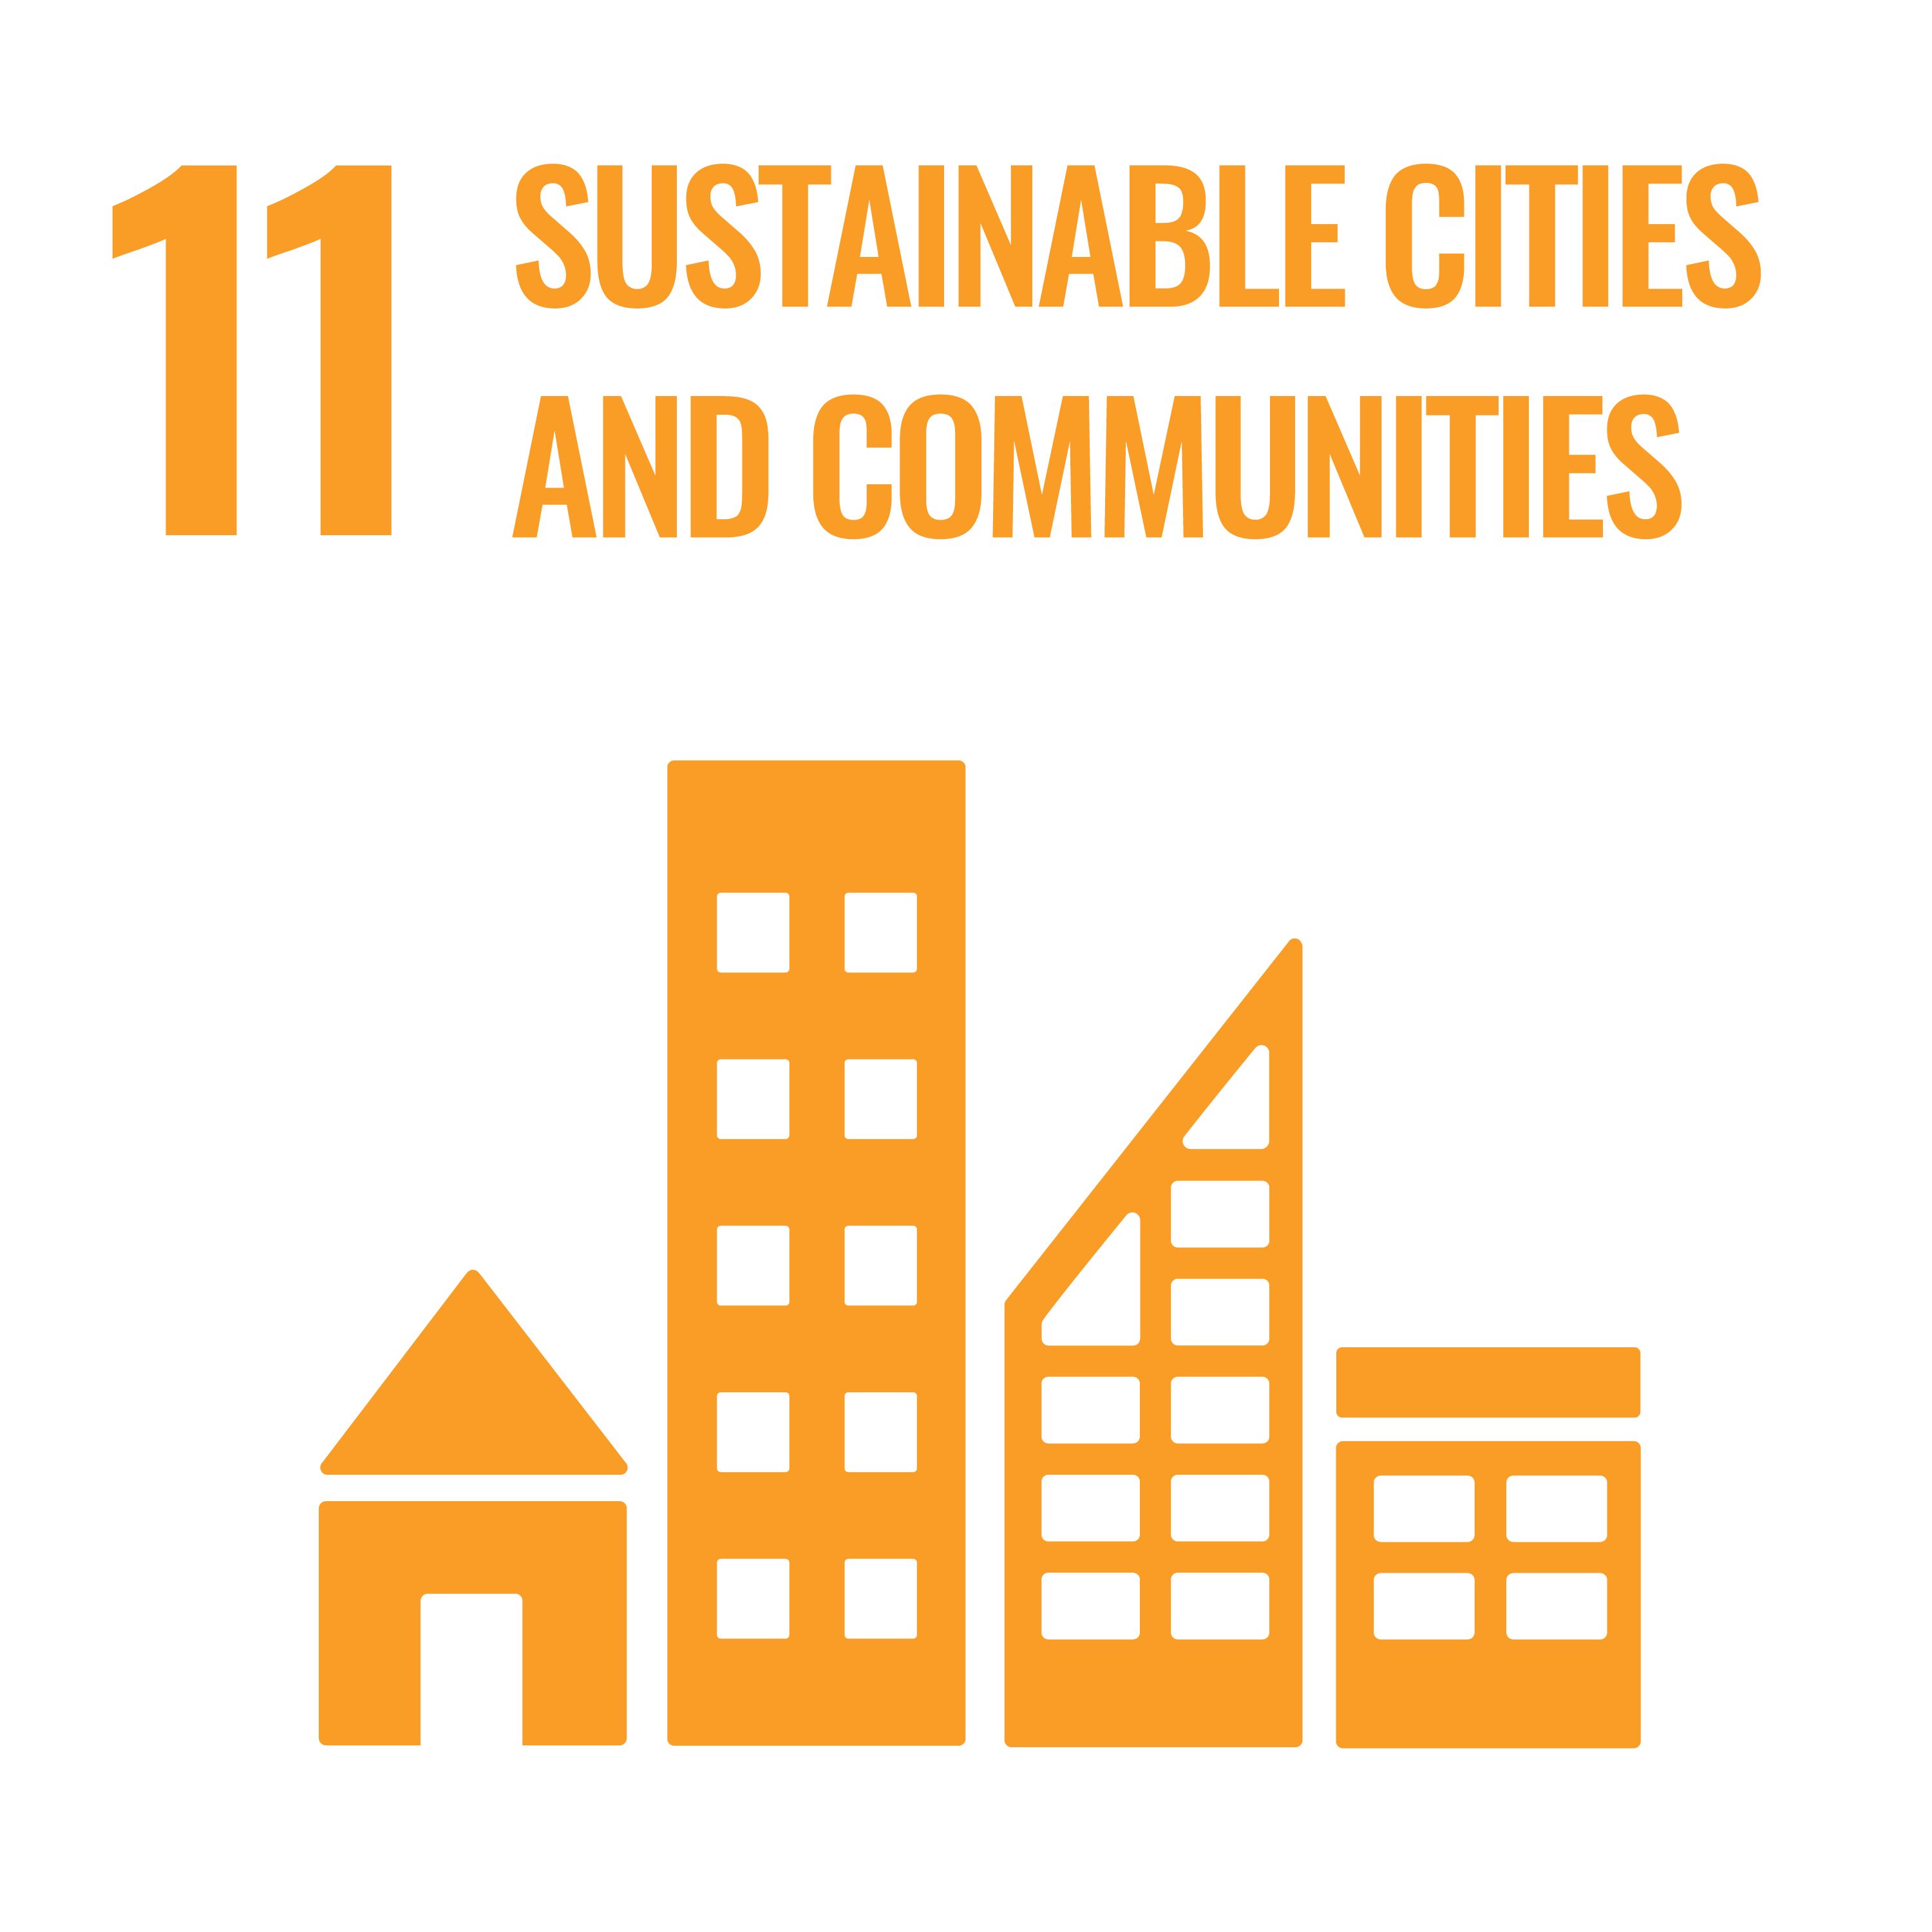
\includegraphics[scale=\SDGscale]{Sections/Figs/Common/SDG_11_SustainableCities.png}}} & \parbox[t]{\SDGright\textwidth}{\textbf{11 Sustainable cities and communities:\ Make cities and human settlements inclusive, safe, resilient, and sustainable}
\vspace{\recskip}
\begin{itemize}[leftmargin=20pt]
\setlength{\itemsep}{\recskip}
\item The campuses of research facilities have an impact on the cities and neighbourhoods in which they are built.
\item The behaviour and lifestyle choices of our community in professional and private life have an impact on our local communities.
\end{itemize}}\\

\parbox[t]{\SDGleft\textwidth}{\raisebox{\iconskip}{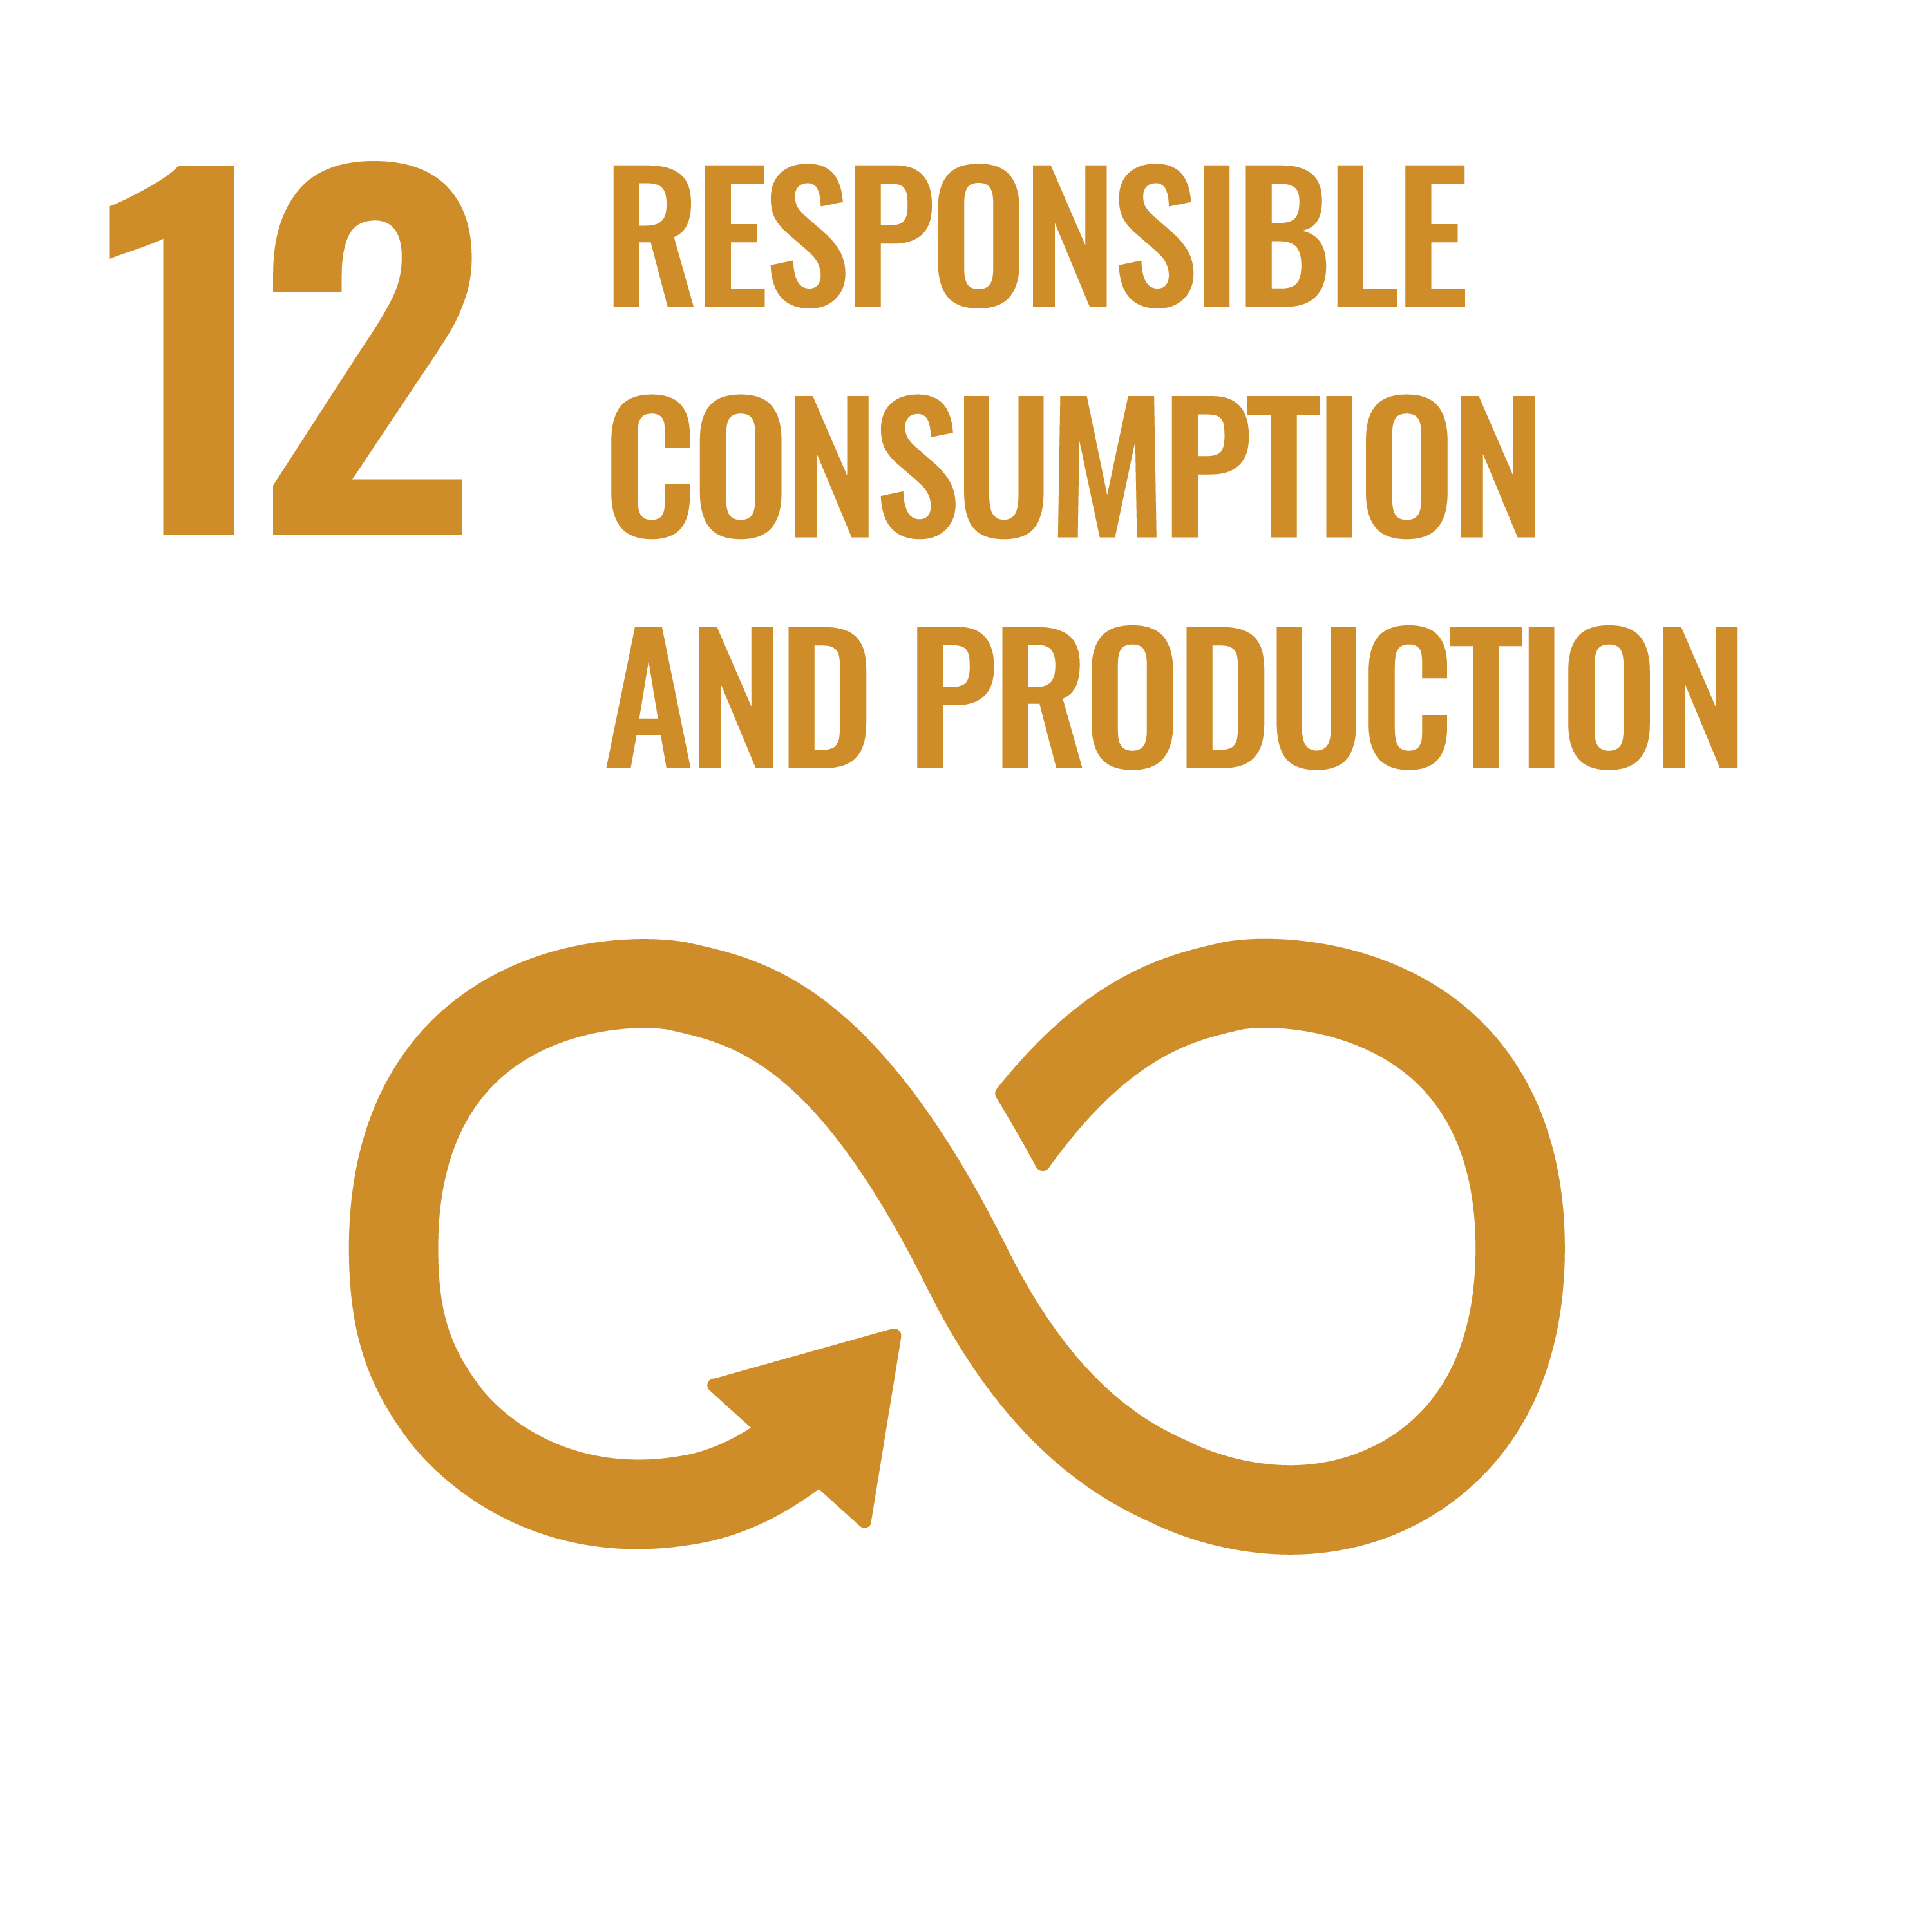
\includegraphics[scale=\SDGscale]{Sections/Figs/Common/SDG_12_ResponsibleConsumption.png}}} & \parbox[t]{\SDGright\textwidth}{\textbf{12 Responsible consumption and production:\ Ensure sustainable consumption and production patterns}
\vspace{\recskip}
\begin{itemize}[leftmargin=20pt]
\setlength{\itemsep}{\recskip}
\item The facilities, accelerators, machines, and experiments we build use up resources and energy in their design, construction, overall lifetime (\eg maintenance) and disposal.
\item The disposal of obsolete equipment and other waste generated by the work we do has an impact on our environment.
\item Our daily choices on consumption have a wider effect on the systems which produce them, \eg food and travel.
\end{itemize}}\\

\parbox[t]{\SDGleft\textwidth}{\raisebox{\iconskip}{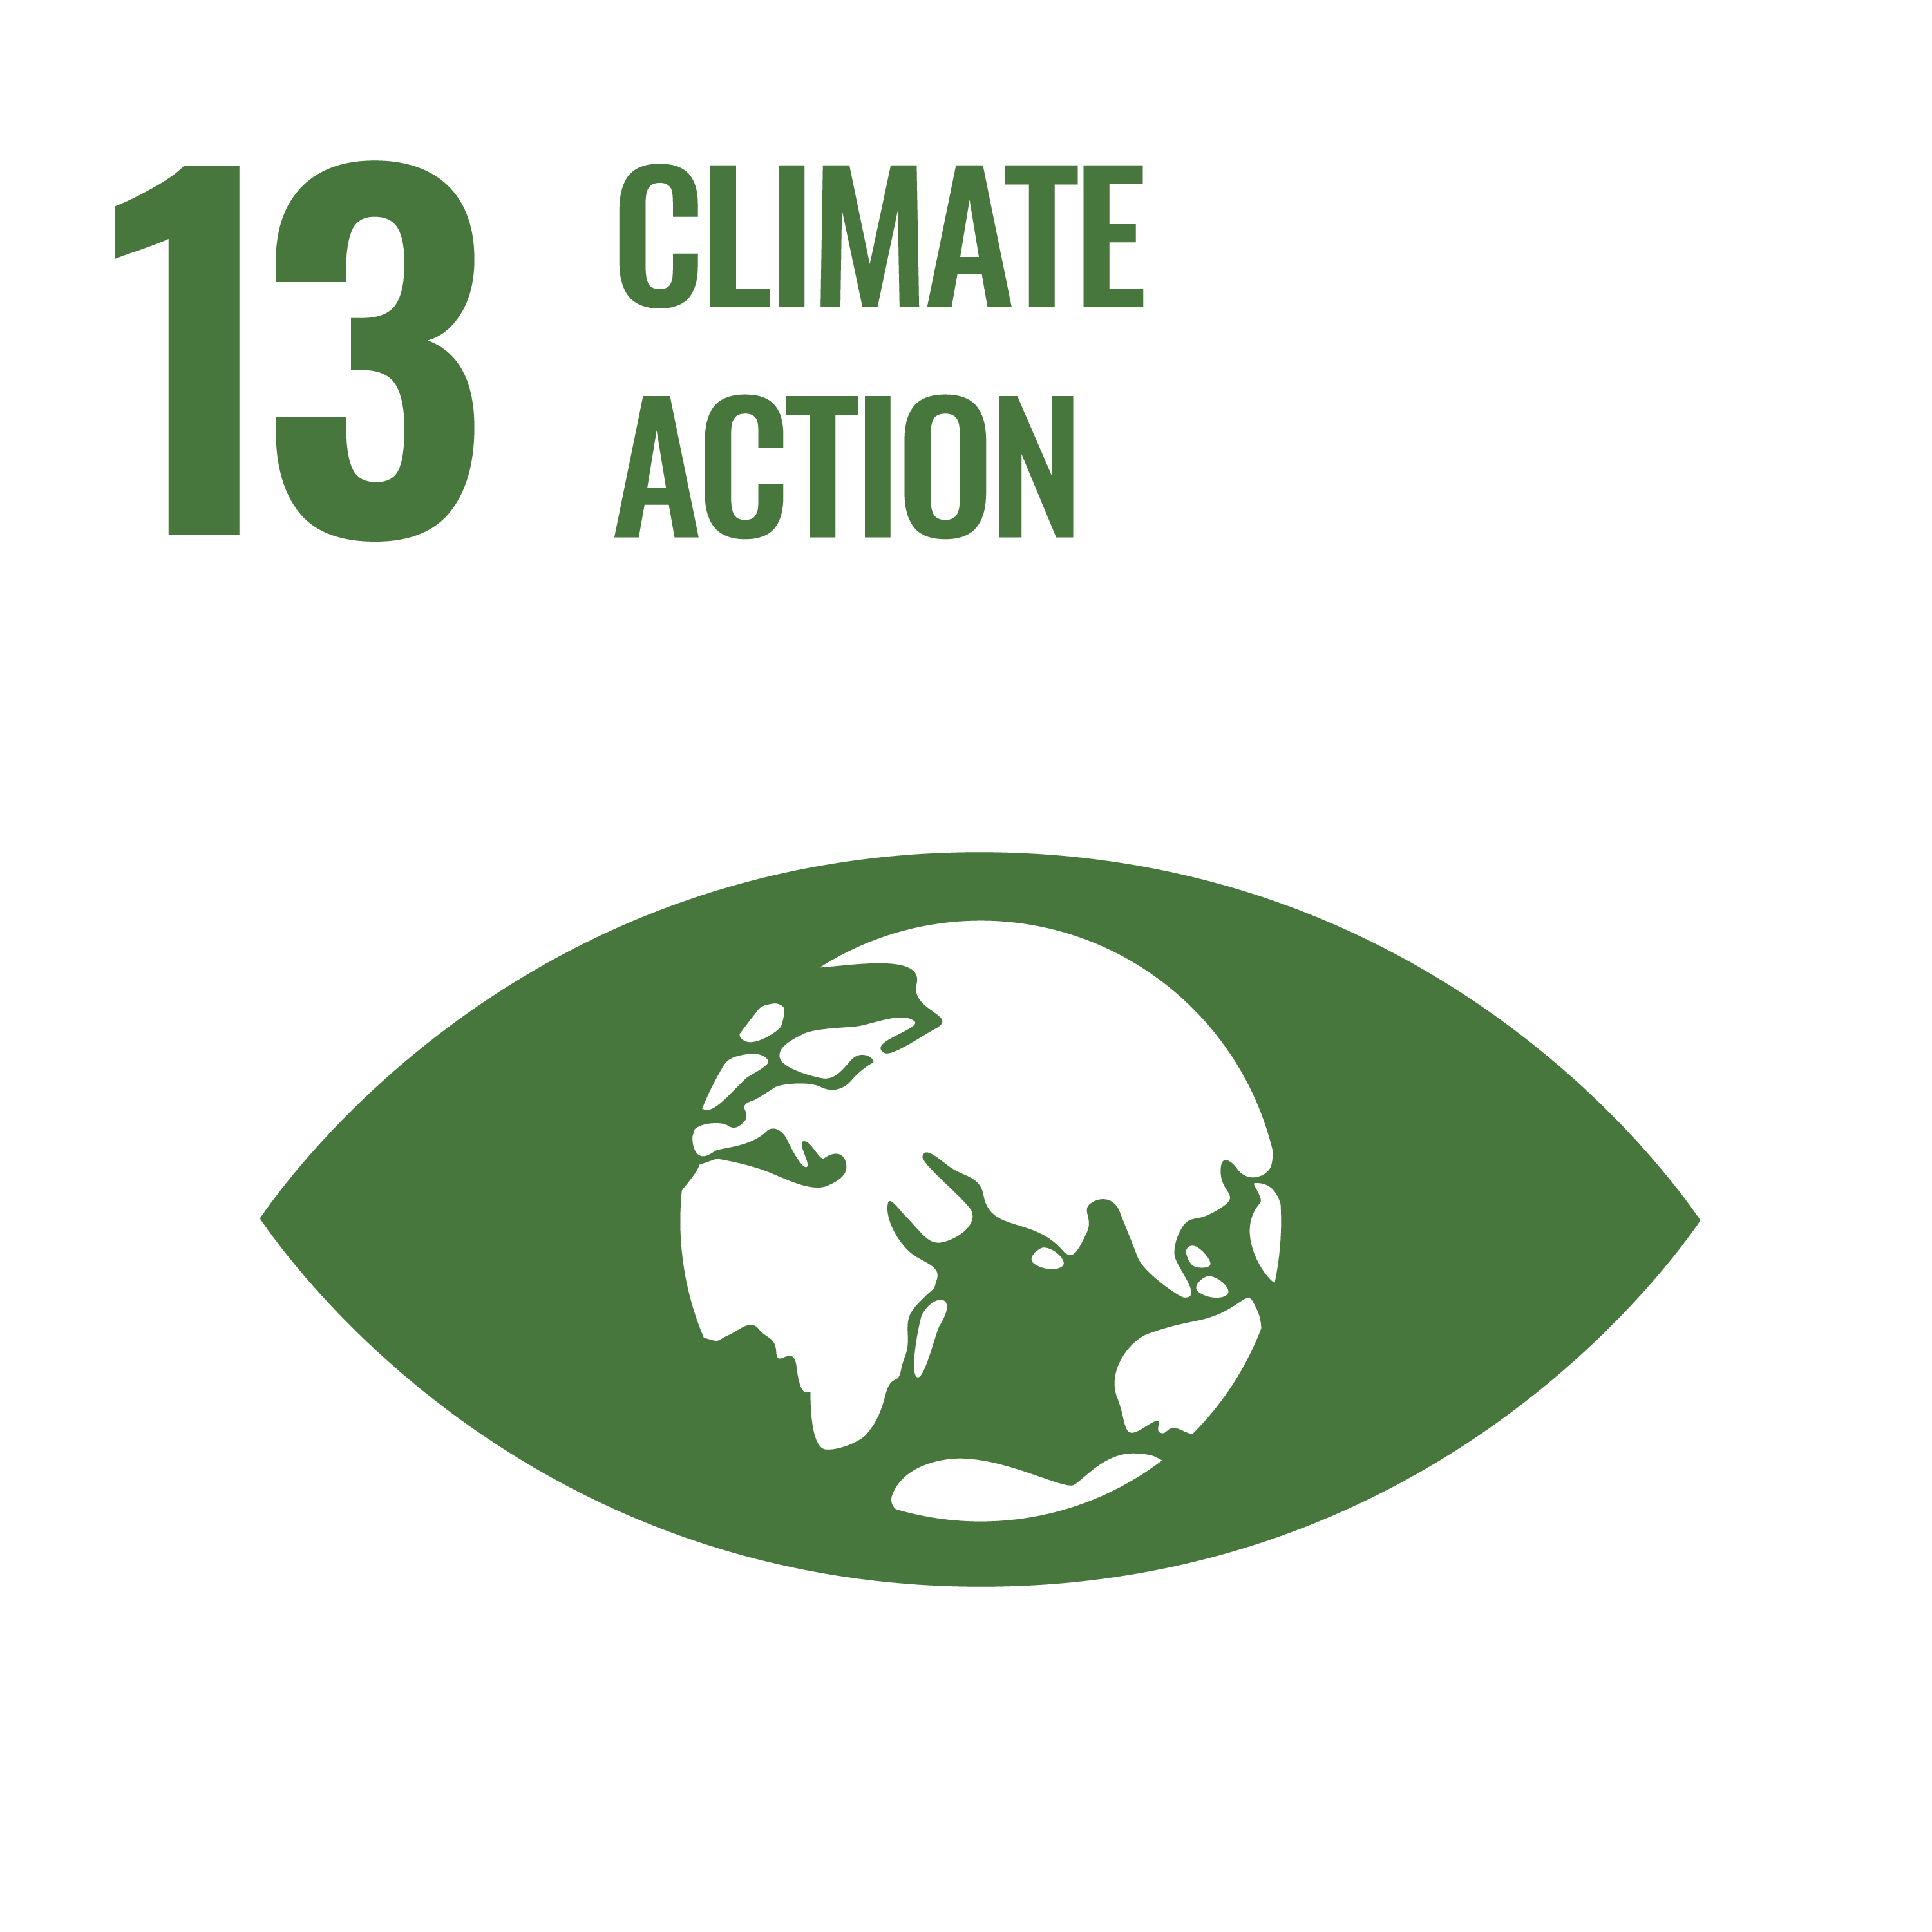
\includegraphics[scale=\SDGscale]{Sections/Figs/Common/SDG_13_ClimateAction.png}}} & \savenotes\parbox[t]{\SDGright\textwidth}{\textbf{13 Climate action:\ Take urgent action to combat climate change and its impacts*}\footnote{Footnote by the UN: *Acknowledging that the United Nations Framework Convention on Climate Change is the primary international, intergovernmental forum for negotiating the global response to climate change.}
\vspace{\recskip}
\begin{itemize}[leftmargin=20pt]
\setlength{\itemsep}{\recskip}
\item The emission of various gases by \ACR\ research has an impact on the Earth’s climate.
\item The sources of the electrical and thermal energy used by \ACR\ facilities impact the global climate.
\item The behaviour and lifestyle choices (eating, travel, product consumption) of our community in professional and private life have an impact on the global climate.
\end{itemize}}\spewnotes\\

\parbox[t]{\SDGleft\textwidth}{\raisebox{\iconskip}{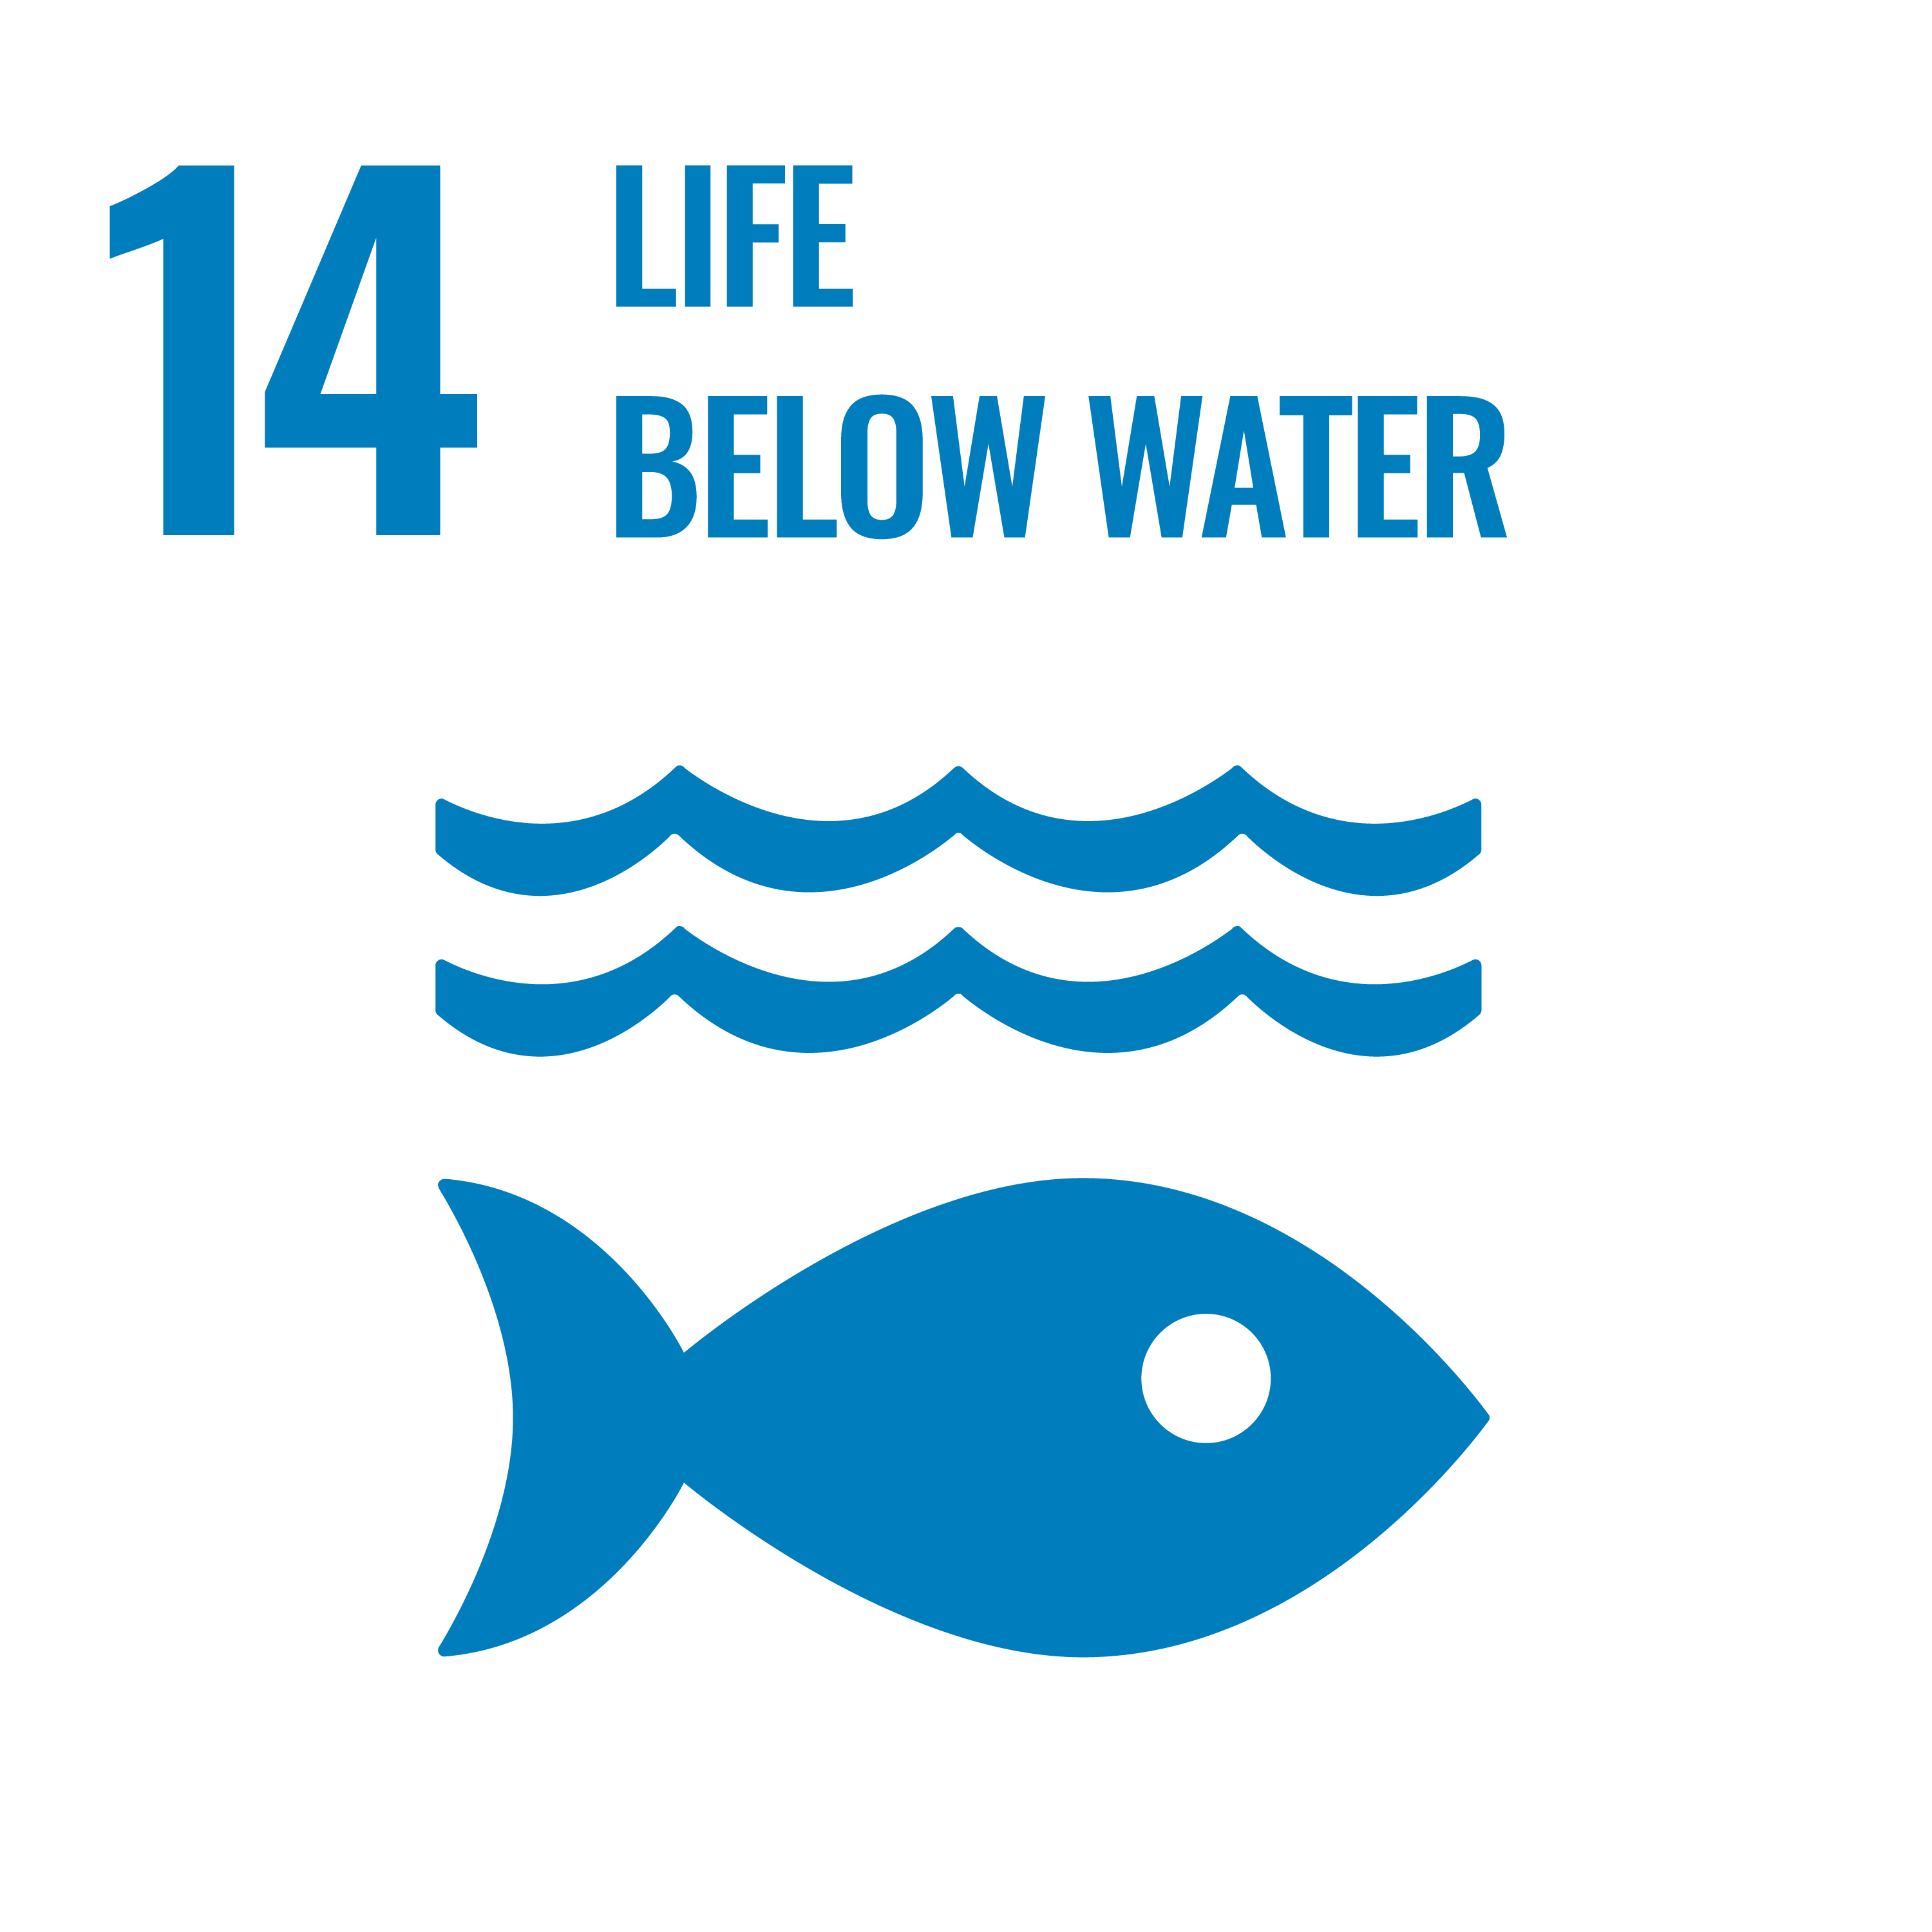
\includegraphics[scale=\SDGscale]{Sections/Figs/Common/SDG_14_LifeBelowWater.png}}} & \parbox[t]{\SDGright\textwidth}{\textbf{14 Life below water:\ Conserve and sustainably use the oceans, seas and marine resources for sustainable development}
\vspace{\recskip}
\begin{itemize}[leftmargin=20pt]
\setlength{\itemsep}{\recskip}
\item Some of the \ACR\ experiments and facilities are built within or close to aquatic ecosystems, \eg Antarctica, and therefore affect these both directly and indirectly.
\item Many goods, products and experiments used in research are travelling the oceans prior to use.
\item The industries that produce the goods that we consume use water and produce waste products, some of which ends up in the ocean.
\item The behaviour and lifestyle choices of our community in professional and private life have an impact on the oceans, through the demand for clean water, and the production of waste water and residues, including microplastics.
\end{itemize}}\\

\parbox[t]{\SDGleft\textwidth}{\raisebox{\iconskip}{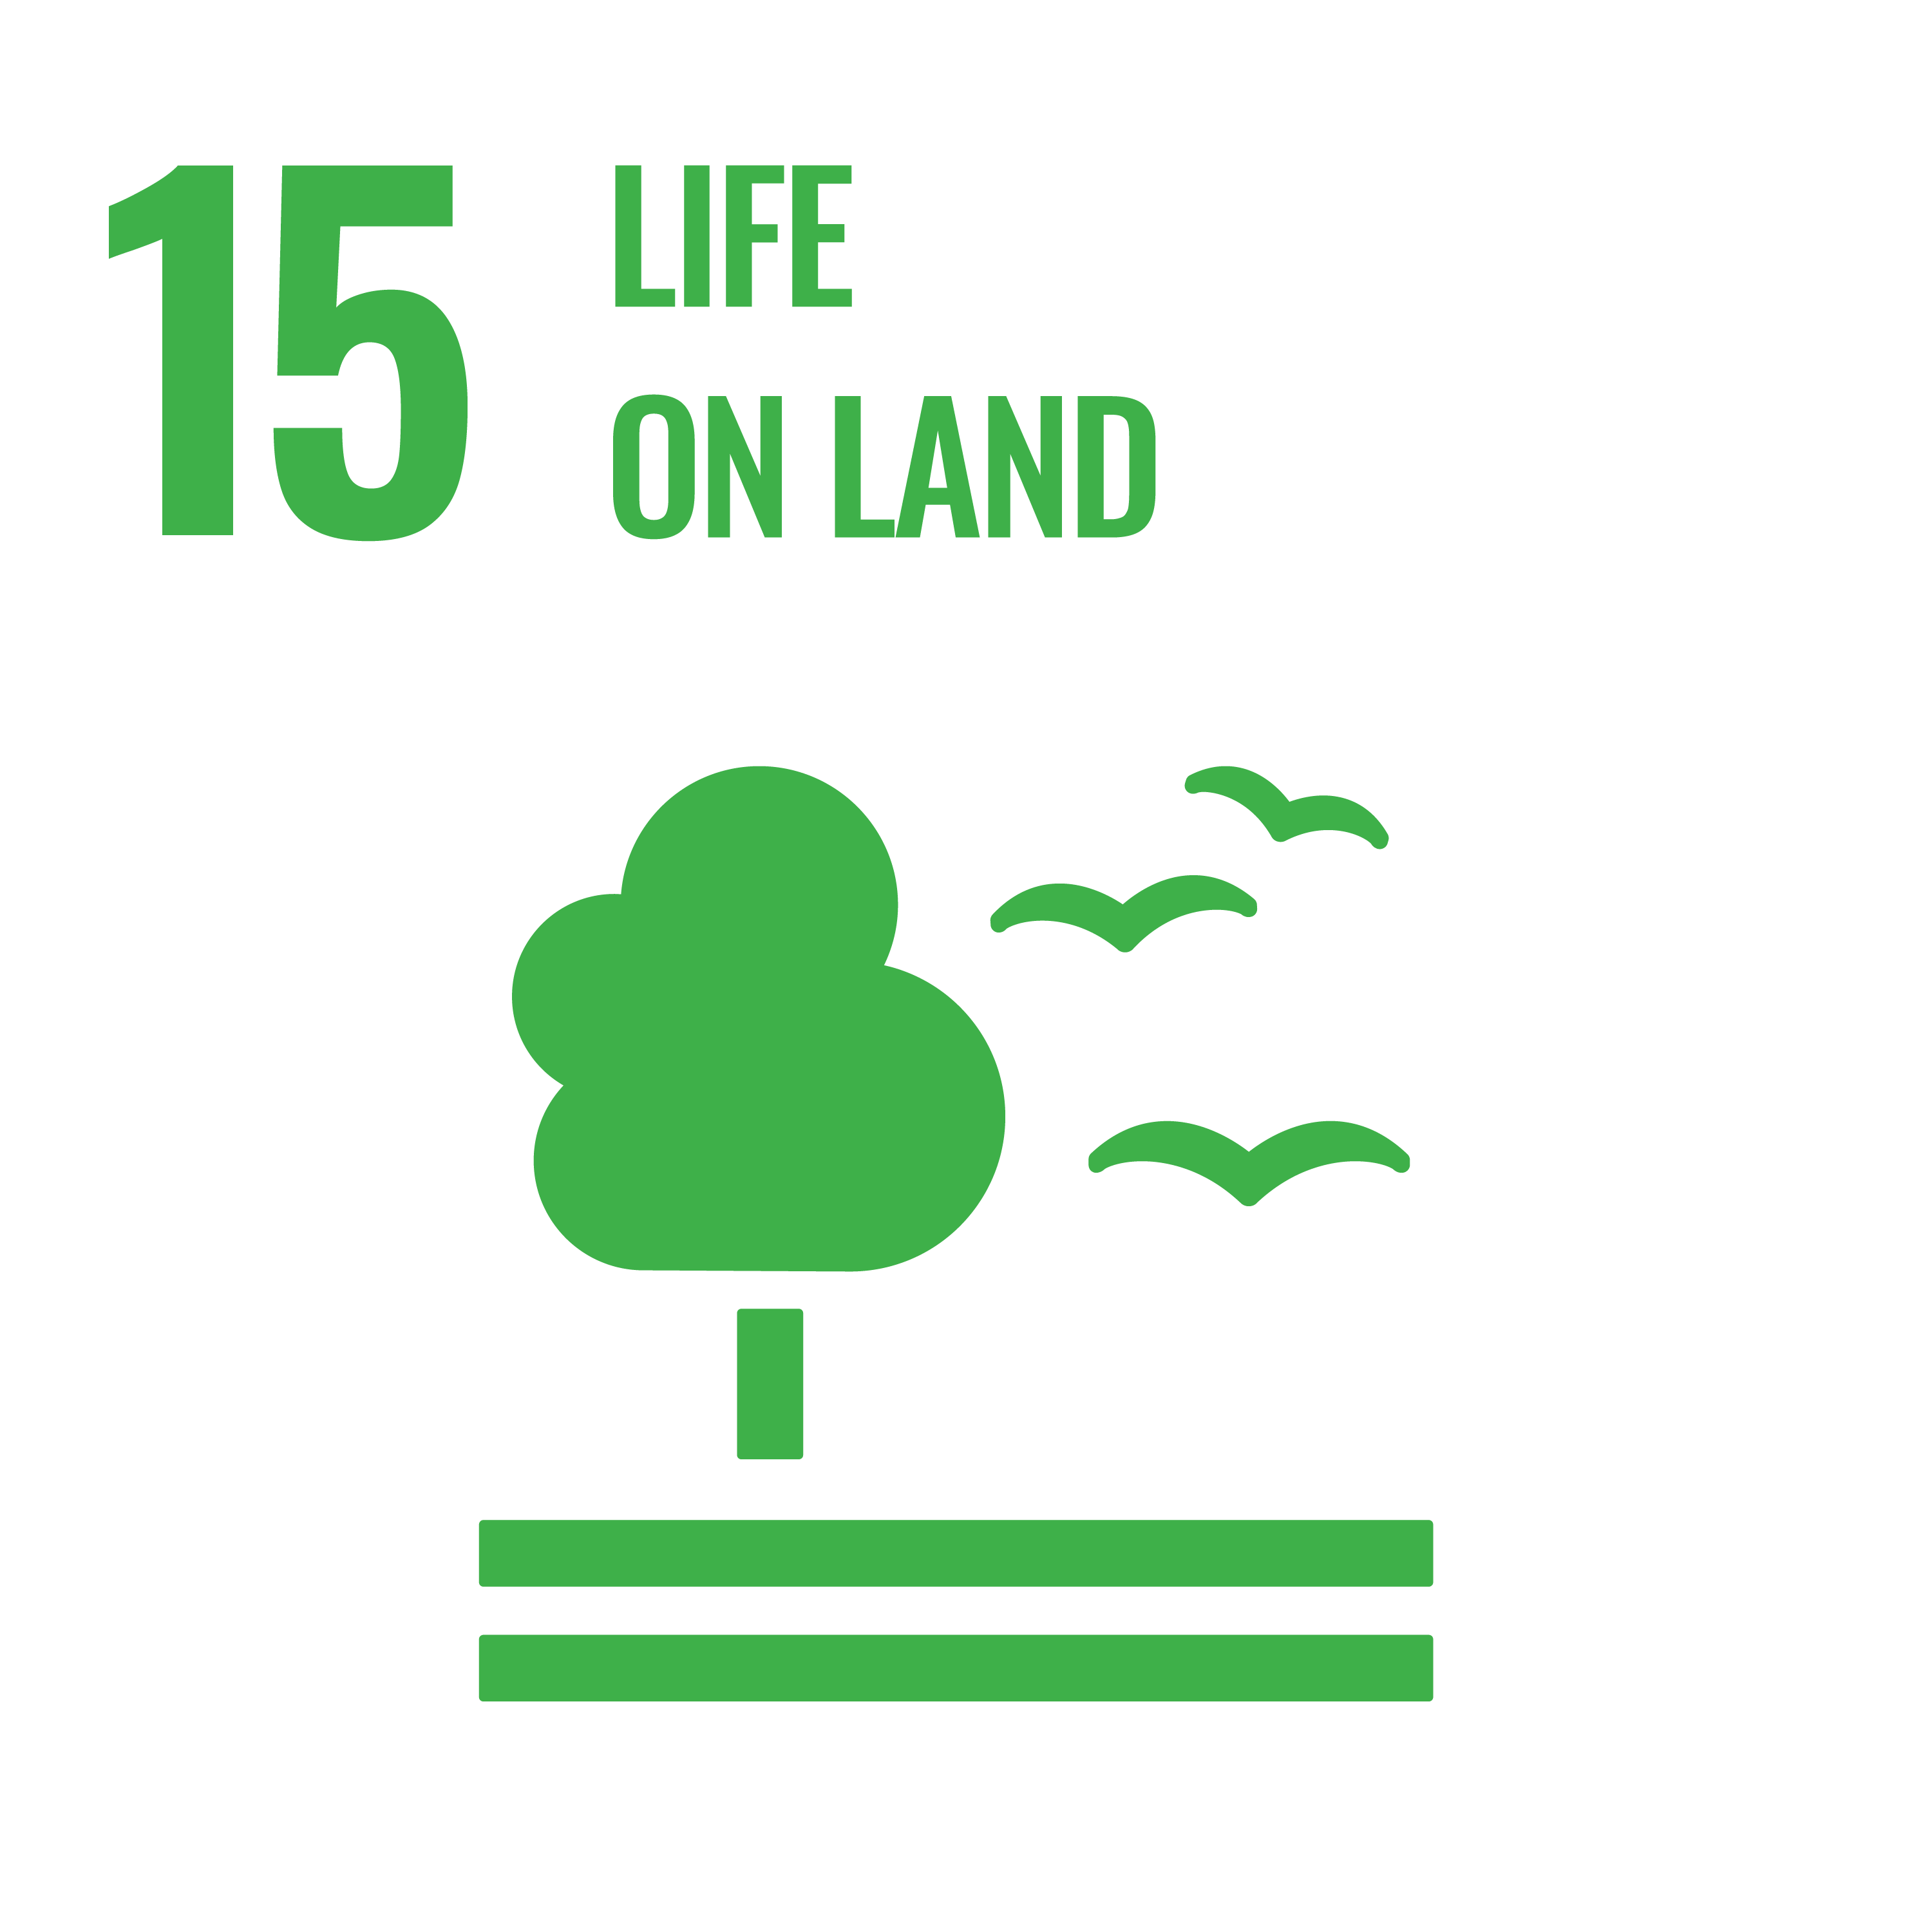
\includegraphics[scale=\SDGscale]{Sections/Figs/Common/SDG_15_LifeOnLand.png}}} & \parbox[t]{\SDGright\textwidth}{\textbf{15 Life on land:\ Protect, restore and promote sustainable use of terrestrial ecosystems, sustainably manage forests, combat desertification, and halt and reverse land degradation and halt biodiversity loss}
\vspace{\recskip}
\begin{itemize}[leftmargin=20pt]
\setlength{\itemsep}{\recskip}
\item Campuses are ecosystems.
\item Expanding the campuses of research institutes can have an impact on surrounding ecosystems.
\item Our consumption has direct (\eg deforestation for agriculture and construction) and indirect (\eg our emissions give rise to more frequent extreme weather events) effects on land use, damaging ecosystems.
\item The behaviour and lifestyle choices of our community in professional and private life have an impact on the land and its ecosystems, because of the extraction of resources and the production of waste or residues.
\end{itemize}}\\

\parbox[t]{\SDGleft\textwidth}{\raisebox{\iconskip}{
\includegraphics[scale=\SDGscale]{Sections/Figs/Common/SDG_16_PeaceJusticeStrongInstitutions.png}}} & \parbox[t]{\SDGright\textwidth}{\textbf{16 Peace, justice and strong institutions:\ Promote peaceful and inclusive societies for sustainable development, provide access to justice for all and build effective, accountable and inclusive institutions at all levels}
\vspace{\recskip}
\begin{itemize}[leftmargin=20pt]
\setlength{\itemsep}{\recskip}
\item \ACR\ is an international field demonstrating harmonious partnership in working towards common goals, and can serve as a model for peaceful international collaboration.
\item \ACR\ is part of society, and it is composed of institutions that can help shape the societies and politics within which they are embedded.
\item Large-scale \ACR\ projects can have a positive impact on industrial and political partnerships.
\item Transparent reporting on efforts towards more sustainable research has a positive impact on the credibility of scientists, and helps avoid greenwashing.
\end{itemize}}\\

\parbox[t]{\SDGleft\textwidth}{\raisebox{\iconskip}{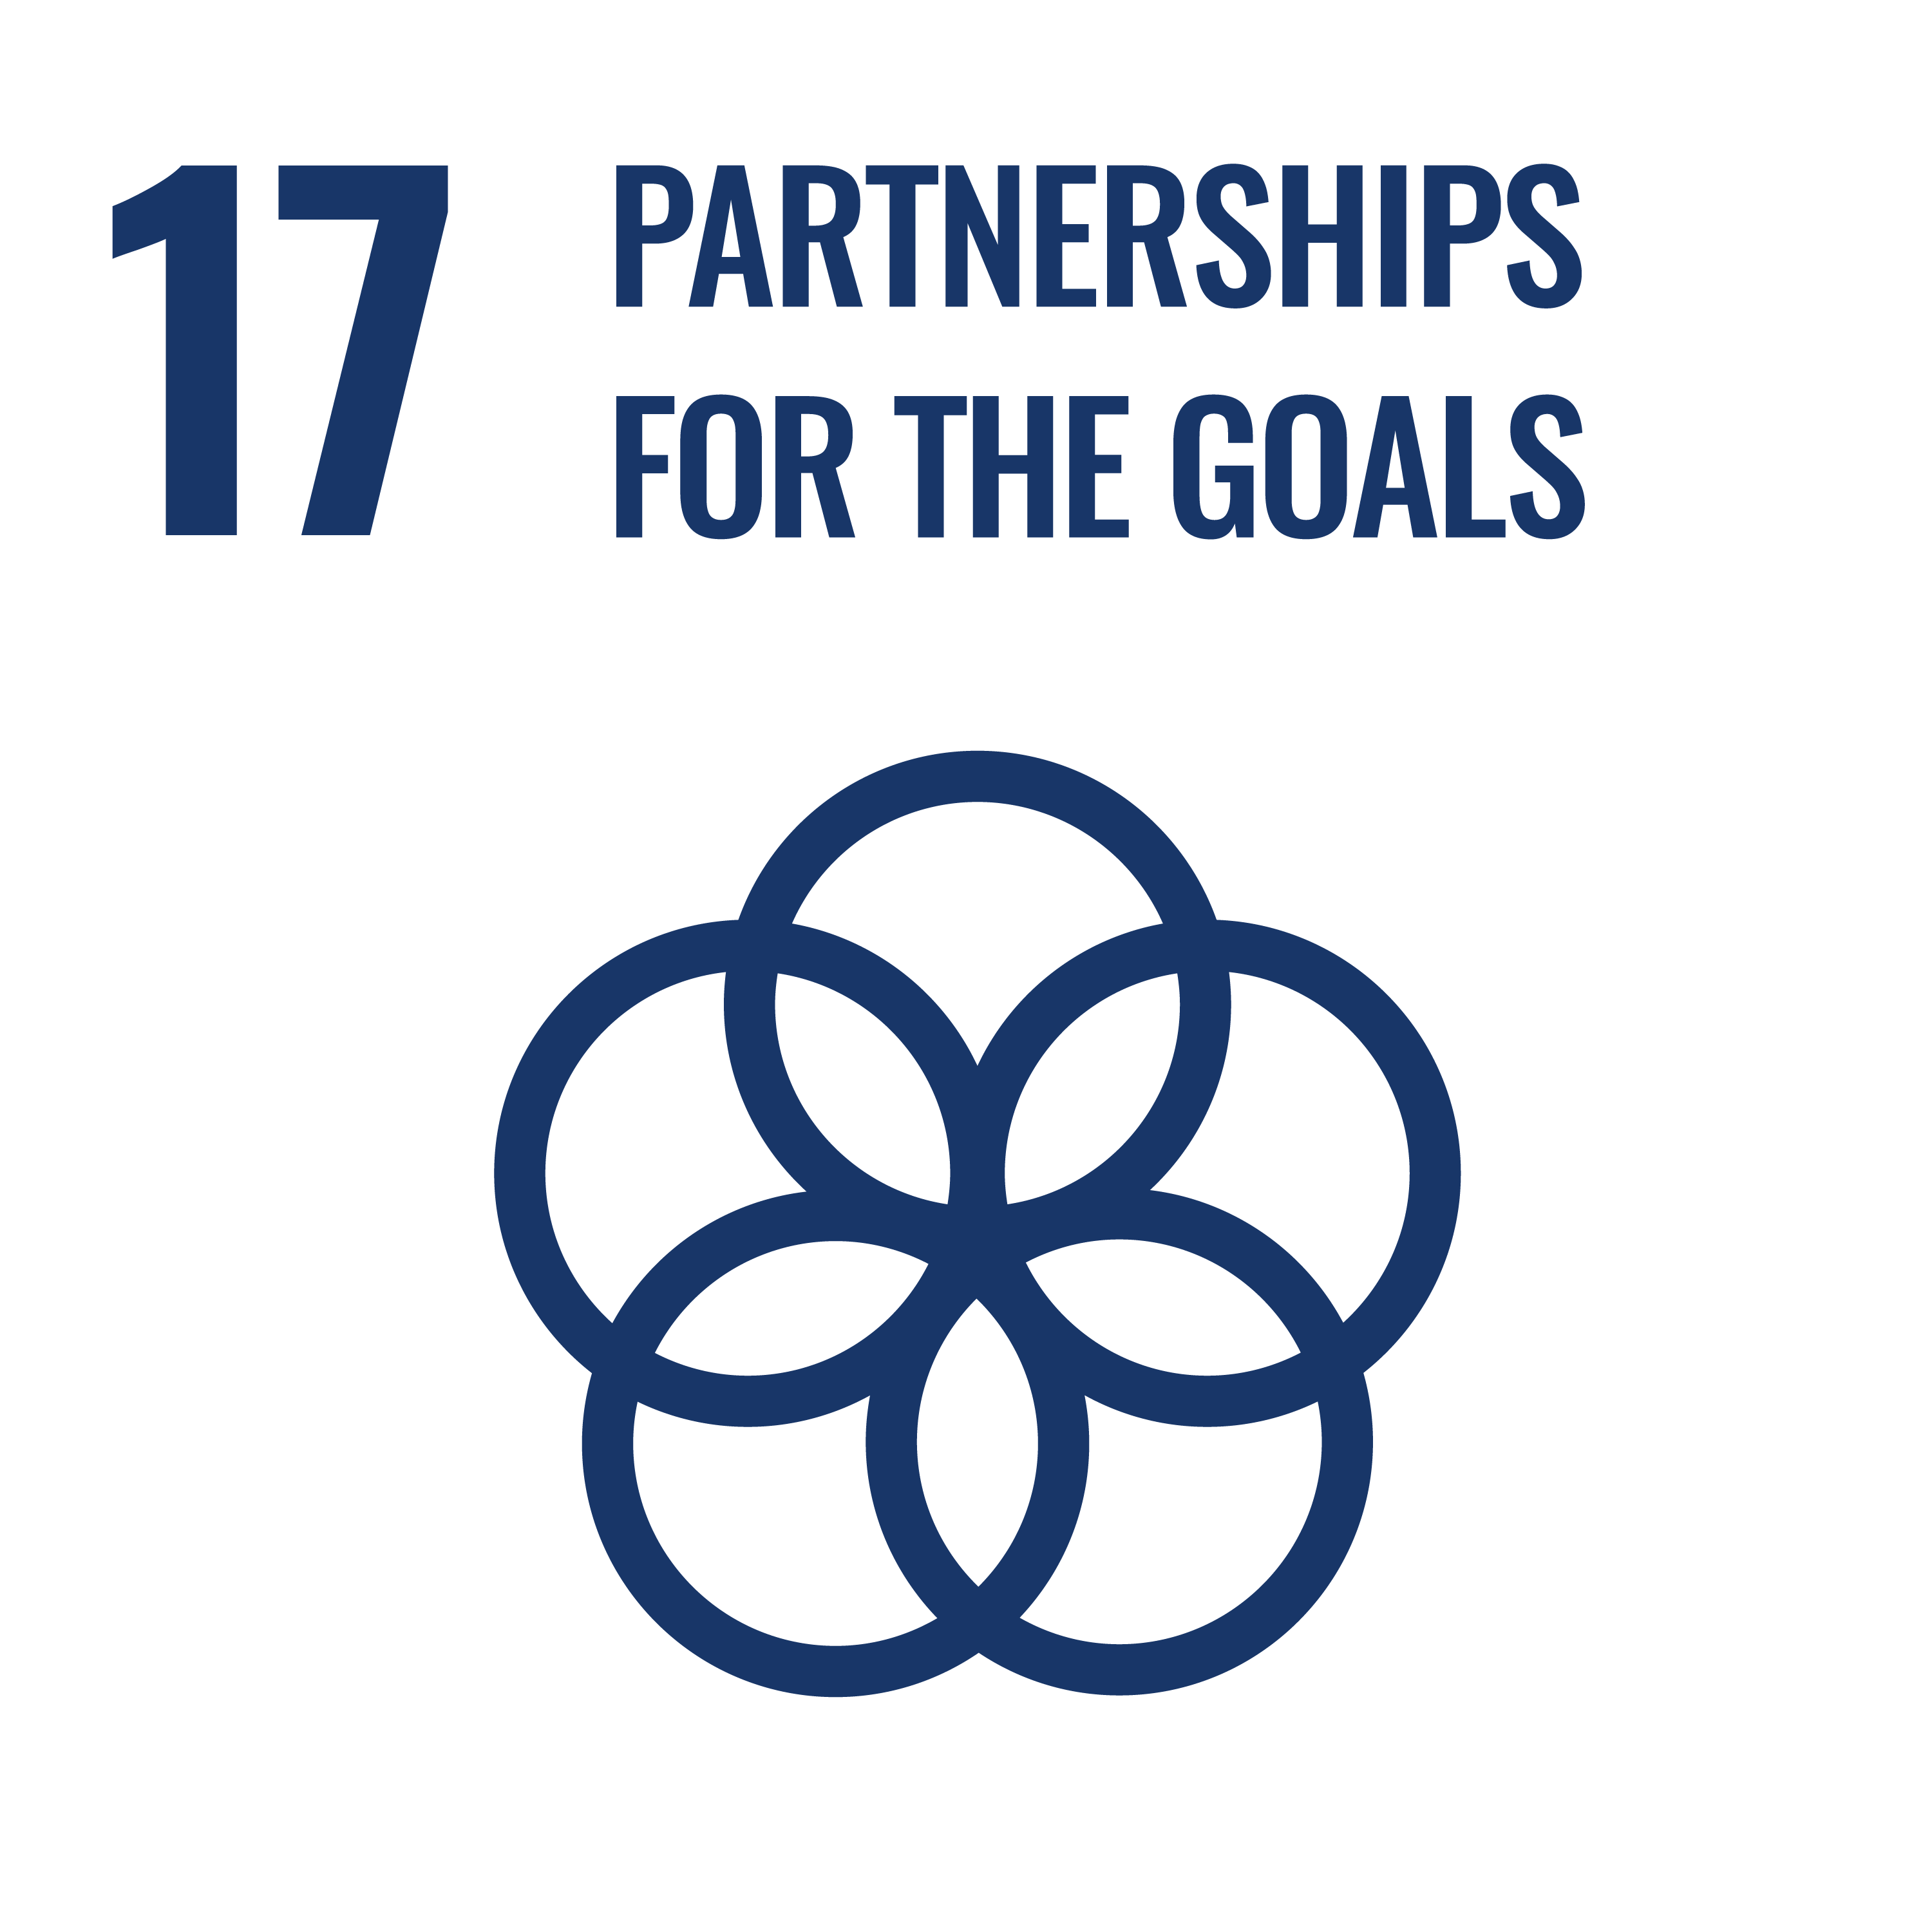
\includegraphics[scale=\SDGscale]{Sections/Figs/Common/SDG_17_PartnershipForGoals.png}}} & \parbox[t]{\SDGright\textwidth}{\textbf{17 Partnership for the Goals:\ Strengthen the means of implementation and revitalize the global partnership for sustainable development}
\vspace{\recskip}
\begin{itemize}[leftmargin=20pt]
\setlength{\itemsep}{\recskip}
\item As an international community based on research and a driver for innovation, we can influence our partners and work together to strengthen a sustainable society around the globe.
\end{itemize}}

\end{longtable*}
\renewcommand*{\arraystretch}{1}

\end{document}